\documentclass[twoside]{book}

% Packages required by doxygen
\usepackage{calc}
\usepackage{doxygen}
\usepackage{graphicx}
\usepackage[utf8]{inputenc}
\usepackage{makeidx}
\usepackage{multicol}
\usepackage{multirow}
\usepackage{textcomp}
\usepackage[table]{xcolor}

% NLS support packages
Portuguese
% Font selection
\usepackage[T1]{fontenc}
\usepackage{mathptmx}
\usepackage[scaled=.90]{helvet}
\usepackage{courier}
\usepackage{amssymb}
\usepackage{sectsty}
\renewcommand{\familydefault}{\sfdefault}
\allsectionsfont{%
  \fontseries{bc}\selectfont%
  \color{darkgray}%
}
\renewcommand{\DoxyLabelFont}{%
  \fontseries{bc}\selectfont%
  \color{darkgray}%
}

% Page & text layout
\usepackage{geometry}
\geometry{%
  a4paper,%
  top=2.5cm,%
  bottom=2.5cm,%
  left=2.5cm,%
  right=2.5cm%
}
\tolerance=750
\hfuzz=15pt
\hbadness=750
\setlength{\emergencystretch}{15pt}
\setlength{\parindent}{0cm}
\setlength{\parskip}{0.2cm}
\makeatletter
\renewcommand{\paragraph}{%
  \@startsection{paragraph}{4}{0ex}{-1.0ex}{1.0ex}{%
    \normalfont\normalsize\bfseries\SS@parafont%
  }%
}
\renewcommand{\subparagraph}{%
  \@startsection{subparagraph}{5}{0ex}{-1.0ex}{1.0ex}{%
    \normalfont\normalsize\bfseries\SS@subparafont%
  }%
}
\makeatother

% Headers & footers
\usepackage{fancyhdr}
\pagestyle{fancyplain}
\fancyhead[LE]{\fancyplain{}{\bfseries\thepage}}
\fancyhead[CE]{\fancyplain{}{}}
\fancyhead[RE]{\fancyplain{}{\bfseries\leftmark}}
\fancyhead[LO]{\fancyplain{}{\bfseries\rightmark}}
\fancyhead[CO]{\fancyplain{}{}}
\fancyhead[RO]{\fancyplain{}{\bfseries\thepage}}
\fancyfoot[LE]{\fancyplain{}{}}
\fancyfoot[CE]{\fancyplain{}{}}
\fancyfoot[RE]{\fancyplain{}{\bfseries\scriptsize Gerado em Quarta, 3 de Setembro de 2014 20:41:59 para proVANT-RemoteControlledFlight por Doxygen }}
\fancyfoot[LO]{\fancyplain{}{\bfseries\scriptsize Gerado em Quarta, 3 de Setembro de 2014 20:41:59 para proVANT-RemoteControlledFlight por Doxygen }}
\fancyfoot[CO]{\fancyplain{}{}}
\fancyfoot[RO]{\fancyplain{}{}}
\renewcommand{\footrulewidth}{0.4pt}
\renewcommand{\chaptermark}[1]{%
  \markboth{#1}{}%
}
\renewcommand{\sectionmark}[1]{%
  \markright{\thesection\ #1}%
}

% Indices & bibliography
\usepackage{natbib}
\usepackage[titles]{tocloft}
\setcounter{tocdepth}{3}
\setcounter{secnumdepth}{5}
\makeindex

% Hyperlinks (required, but should be loaded last)
\usepackage{ifpdf}
\ifpdf
  \usepackage[pdftex,pagebackref=true]{hyperref}
\else
  \usepackage[ps2pdf,pagebackref=true]{hyperref}
\fi
\hypersetup{%
  colorlinks=true,%
  linkcolor=blue,%
  citecolor=blue,%
  unicode%
}

% Custom commands
\newcommand{\clearemptydoublepage}{%
  \newpage{\pagestyle{empty}\cleardoublepage}%
}


%===== C O N T E N T S =====

\begin{document}

% Titlepage & ToC
\hypersetup{pageanchor=false}
\pagenumbering{roman}
\begin{titlepage}
\vspace*{7cm}
\begin{center}%
{\Large pro\-V\-A\-N\-T-\/\-Remote\-Controlled\-Flight \\[1ex]\large 0.\-3 }\\
\vspace*{1cm}
{\large Gerado por Doxygen 1.8.4}\\
\vspace*{0.5cm}
{\small Quarta, 3 de Setembro de 2014 20:41:59}\\
\end{center}
\end{titlepage}
\clearemptydoublepage
\tableofcontents
\clearemptydoublepage
\pagenumbering{arabic}
\hypersetup{pageanchor=true}

%--- Begin generated contents ---
\chapter{Página principal}
\label{index}\hypertarget{index}{}\hypertarget{index_page_main_sec_overview}{}\section{Overview}\label{index_page_main_sec_overview}
Este é a documentacão do projeto de software {\bfseries Remote Controlled Flight} do {\bfseries pro\-V\-A\-N\-T}. O objetivo deste projeto de software é gerar um firmware para a {\itshape io-\/board} do V\-A\-N\-T que permita operá-\/lo com um controle remoto convencional de aeromodelismo. Para tal, são necessárias/previstas o seguinte conjunto de finalidades\-:
\begin{DoxyItemize}
\item Comunicação com controle remoto convecional de modelismo, com leitura de 6 ou mais canais via interface P\-P\-M.
\item Funcionalidade completa dos E\-S\-Cs e Servo-\/motores do V\-A\-N\-T.
\item Leitura e tratamento simplificado de dados de uma I\-M\-U (a ser escolhida).
\item Algoritmo de controle garantindo estabilidade rotacional para o V\-A\-N\-T durante o vôo.
\end{DoxyItemize}\hypertarget{index_page_main_sec_changelog}{}\section{Changelog}\label{index_page_main_sec_changelog}
$<$$>$Changelog da versão 0.\-3 \mbox{[}Apr-\/2013\mbox{]} \-:
\begin{DoxyItemize}
\item ...
\item ...
\end{DoxyItemize}

{\bfseries Changelog da versão 0.\-2 \mbox{[}Fev-\/2014 $>$ Mar-\/2014\mbox{]} \-:}
\begin{DoxyItemize}
\item Resolvidas as pendências da versão 0.\-1.
\item Implementada a troca de mensagens entre módulos (em threadas).
\item Atuação\-: Implementado os drivers para o servo R\-X24f e o E\-S\-C da Mikrokopter
\item Sensoriamento\-:
\end{DoxyItemize}

{\bfseries Status da versão 0.\-1 \mbox{[}Nov-\/2013 $>$ Jan-\/2014\mbox{]} \-:}
\begin{DoxyItemize}
\item Implementado o esqueleto básico da estrutura do projeto (sistema de {\bfseries modules} com um {\itshape main} e um {\itshape common})
\item Adotada uma convenção de nomenclatura, descrita em \hyperlink{page_naming}{Organização, nomenclaturas e code-\/style} )
\item Implementadas as funções básicas para\-:
\begin{DoxyItemize}
\item U\-S\-A\-R\-T (2 e 6; 3 ainda pendente) com tratador de interrupção e buffer circular.
\item I2\-C (I2\-C1)
\item G\-P\-I\-O (wrappers) e E\-X\-T\-I (interrupts externos)
\end{DoxyItemize}
\item Implementados módulos para\-:
\begin{DoxyItemize}
\item Receiver (usando T\-I\-M1 e E\-X\-T\-I)
\item Servo R\-X24\-F, portando a biblioteca preexistente do Arduino.
\item I2\-C (exemplo com I\-M\-U simples baseada nos C\-Is I\-T\-G3205 e A\-D\-X\-L345)
\end{DoxyItemize}
\item Integração com Free\-R\-T\-O\-S.
\item Integração e teste com \href{http://www.freertos.org/FreeRTOS-Plus/FreeRTOS_Plus_Trace/FreeRTOS_Plus_Trace.shtml}{\tt Free\-R\-T\-O\-S+\-Trace} e Tracealyzer, ver \hyperlink{page_freertosplustrace}{Usando o Free\-R\-T\-O\-S + Trace} .
\end{DoxyItemize}

{\bfseries Pendências da versão 0.\-1\-:}
\begin{DoxyItemize}
\item Atualizar a documentação (decritivo da estrutura de projeto, em \hyperlink{page_naming}{Organização, nomenclaturas e code-\/style} )
\item Implementar troca de mensagens entre threads.
\end{DoxyItemize}

Para pendências internas no código, ver lista de tarefas auto-\/gerada (todo ). 
\chapter{Organização, nomenclaturas e code-\/style}
\label{page_naming}
\hypertarget{page_naming}{}
\hypertarget{page_naming_page_naming_sec_codeorganization}{}\section{Organização deste projeto}\label{page_naming_page_naming_sec_codeorganization}
Este projeto tenta seguir os princípios de organização apresentados em {\itshape  \href{http://www.amazon.com/Large-Scale-Software-Design-John-Lakos/dp/0201633620}{\tt Large-\/\-Scale C++ Software Design}}, de John Lakos. Para tal, tentou-\/se implementar uma estrutura hierárquica verticalizada dos elementos de um nível em relação aos de um nível superior. Para a descrição deste projeto, faz-\/se necessário apresentar convenções de nomenclatura usadas pelo autor, adaptadas ao contexto desta aplicação. São elas\-:

\begin{center} \begin{TabularC}{2}
\hline
\rowcolor{lightgray}{\bf Nomenclatura }&{\bf Uso em contexto  }\\\cline{1-2}
Arquivo &Unidade atômica do projeto; conjuntos de dados com extensões ({\itshape .c, .cpp, .h, etc }), ou binários sem extensão. \\\cline{1-2}
Componente &Par de arquivos; {\itshape  header + source file } respectivos. Exemplo, {\ttfamily c\-\_\-io\-\_\-imu.\-c} e {\ttfamily c\-\_\-io\-\_\-imu.\-h}. Pode ser referido como {\bfseries submódulo}. \\\cline{1-2}
Módulo &Conjunto de componentes implementando alguma unidade funcional. Exemplo, a coleção de arquivos em {\itshape  modules/io }, que implementa as funções de E/\-S do V\-A\-N\-T. \\\cline{1-2}
Subsistema &Conjunto de módulo + documentação do módulo + unidades de teste do módulo. \\\cline{1-2}
Sistema &Conjunto de subsistemas + documentação + aplicação que implementam a funcionalidade total do V\-A\-N\-T. \\\cline{1-2}
\end{TabularC}
\end{center} 

Neste projeto, a {\bfseries aplicação} -\/ o binário a ser efetivamente executado pelo V\-A\-N\-T -\/, se encontra a nível de {\bfseries sistema}. O uso de documentação independente para os {\bfseries subsistemas} não é necessária no escopo deste projeto, e portanto, toda a documentação dos {\bfseries módulos} é gerada {\itshape juntamente com esta documentação} de {\bfseries sistema}. Durante o uso deste documento, quando estes termos aparecerem com os significados da tabela acima, eles serão marcados em {\bfseries negrito}.

Seguindo um conceito de verticalização, os elementos do projeto estão organizados como no diagrama abaixo\-:



Identificam-\/se três níveis principais e seus elementos, do topo à base\-:


\begin{DoxyItemize}
\item {\bfseries  Application level }
\begin{DoxyItemize}
\item {\itshape Modules\-:} Módulos, implementando as funções de interesse do V\-A\-N\-T (estabilização, navegação, comunicação com {\itshape main-\/board}, etc). O binário da {\bfseries aplicação} é compilado diretamente acima deste nível.
\end{DoxyItemize}
\item {\bfseries  Middleware level }
\begin{DoxyItemize}
\item {\itshape Libs\-:} Bibliotecas próprias ou de terceiros. Funções utilitárias próprias do projeto (a exemplo dos componente {\ttfamily c\-\_\-common\-\_\-utils.\-h} e {\ttfamily c\-\_\-common\-\_\-utils.\-c}) além de bibliotecas como o Tracealyzer estão neste nível.
\item {\itshape H\-A\-L\-:} Hardware Abstraction Layer.
\item {\itshape State-\/\-Machine}\-:
\item {\itshape Free-\/\-R\-T\-O\-S}\-:
\end{DoxyItemize}
\item {\bfseries  Core level }
\begin{DoxyItemize}
\item {\itshape C\-M\-S\-I\-S} {\itshape Core\-:} 
\item {\itshape C\-M\-S\-I\-S} {\itshape Vendor\-:} 
\end{DoxyItemize}
\end{DoxyItemize}

É importante lembrar que um elemento em um nível pode depender direta ou indiretamente de todos os elementos abaixo dele, sem que os princípios de modularidade ou hierarquia vertical sejam violados. No entanto, relações diretas -\/ de um elemento apenas com aqueles diretamente abaixo dele -\/ são recomendadas.\hypertarget{page_naming_page_naming_subsec_foldertree}{}\subsection{Estrutura de pastas}\label{page_naming_page_naming_subsec_foldertree}
Lorem ipsum dolor sit amet, consectetur adipisicing elit, sed do eiusmod tempor incididunt ut labore et dolore magna aliqua. Ut enim ad minim veniam, quis adnum,\hypertarget{page_naming_page_naming_sec_naming}{}\section{Nomenclatura}\label{page_naming_page_naming_sec_naming}
\hypertarget{page_naming_page_naming_subsec_filenaming}{}\subsection{Arquivos e módulos}\label{page_naming_page_naming_subsec_filenaming}
Todos os componentes são nomeados seguindo o padrão\-:


\begin{DoxyCode}
c\_<nome\_do\_modulo>\_<nomeDoComponente>.c
c\_<nome\_do\_modulo>\_<nomeDoComponente>.h 
\end{DoxyCode}


Componentes nomeados desta maneira não devem ser incluídos por arquivos fora do módulo respectivo (como se fossem funcões {\bfseries private}). Componentes públicos de cada módulo (que serão efetivamente incluídos por outros módulos, ou pela {\itshape main}) são nomeados com a sigla {\itshape \char`\"{}pv\char`\"{}} (como em {\bfseries pro\-V\-A\-N\-T}) no início\-:


\begin{DoxyCode}
pv\_interface\_<nomeDoModulo>.\{h,c\}
pv\_module\_<nomeDoModulo>.\{h,c\} 
\end{DoxyCode}


É desejado que o módulo tenha um nome compacto -\/ de preferência uma única palavra ou sigla (ex.\-: {\bfseries rc}, {\bfseries io}, {\bfseries common}) -\/ totalmente minúsculo (ou dividida com letras maísculas e minúsculas; {\itshape \char`\"{}nome\-Do\-Modulo\char`\"{}}). Acentos e caracteres especiais não devem ser usados.

Todos os arquivos do projeto devem incluir uma descrição formatada do Doxygen no topo, com nome, data de criação do arquivo e breve descrição, como segue -\/ exemplo do arquivo {\itshape c\-\_\-rc\-\_\-receiver.\-c} \-:


\begin{DoxyCode}
\textcolor{comment}{/**}
\textcolor{comment}{  /******************************************************************************}
\textcolor{comment}{  * @file    modules/rc/c\_rc\_receiver.c}
\textcolor{comment}{  * @author  Martin Vincent Bloedorn}
\textcolor{comment}{  * @version V1.0.0}
\textcolor{comment}{  * @date    30-November-2013}
\textcolor{comment}{  * @brief   Implementação do receiver do controle de rádio manual.}
\textcolor{comment}{  *          Implementa as funções de recebimento, detecção e interpretação do}
\textcolor{comment}{  *          receiver configurado em modo PPM.}
\textcolor{comment}{  /******************************************************************************/}
\end{DoxyCode}


A tag {\bfseries @date} deve conter a data de criação/inserção do arquivo e não será alterada depois disso. A tag {\bfseries @version} é opcional é serve mais para controle local próprio desenvolvedor.

De maneira equivalente, as funções devem ser adicionadas ao grupo de documentação correto do Doxygen via a tag {\bfseries @addtogroup}. Isto deve ser feito {\bfseries apenas} no {\itshape }.c, garantindo que todas as funções implementadas apareçam na documentação. Primeramente, as funções devem ser adicionadas ao componente ao qual elas pertencem. A descrição do grupo fica na sua definição de mais alto nível, ou seja, a definição do componente fica no próprio {\itshape }.c do componente, enquanto que a definição do módulo fica no {\itshape }.c do módulo ({\bfseries pv\-\_\-module\-\_\-\{}...{\bfseries }\}.h). Em seguida, elas são adicionadas ao módulo equivalente. Novamente, o exemplo abaixo é do arquivo {\itshape c\-\_\-rc\-\_\-receiver.\-c} \-:


\begin{DoxyCode}
\textcolor{comment}{/*! @addtogroup Module\_RC}
\textcolor{comment}{  * @\{}
\textcolor{comment}{  */}
  \textcolor{comment}{}
\textcolor{comment}{/** @addtogroup Module\_RC\_Component\_Receiver}
\textcolor{comment}{  }
\textcolor{comment}{ *  Módulo do receiver.}
\textcolor{comment}{  * @\{}
\textcolor{comment}{  */}
\end{DoxyCode}


Analogamente, o arquivo {\itshape pv\-\_\-module\-\_\-rc.\-c} é então adicionado à listagem de módulos do Pro\-V\-A\-N\-T, e possui então a descrição do grupo {\bfseries Module\-\_\-\-R\-C}.


\begin{DoxyCode}
\textcolor{comment}{/** @addtogroup ProVANT\_Modules}
\textcolor{comment}{  * @\{}
\textcolor{comment}{  */}
\textcolor{comment}{}
\textcolor{comment}{/** @addtogroup Module\_RC}
\textcolor{comment}{  * Definição do módulo de controle e comunicação via rádio manual.}
\textcolor{comment}{  * @\{}
\textcolor{comment}{  */}
\end{DoxyCode}


Isto garante que o diagrama da estrutura de projeto gerada pelo Doxygen corresponde à hierarquia planejada. Os exemplos acima geram um diagrama na documentação como o mostrado abaixo\-:

.\hypertarget{page_naming_page_naming_subsec_codenaming}{}\subsection{Funções, variáveis, etc.}\label{page_naming_page_naming_subsec_codenaming}
{\bfseries Variáveis\-:} critério não estrito, mas recomenda-\/se o uso do padrão Java -\/ com separações apenas com letras maiúsculas e minúsculas.


\begin{DoxyCode}
\textcolor{keywordtype}{int} someVariable; 
\end{DoxyCode}


{\bfseries Funções\-:} seguindo o apresentado acima, devem ser separadas com {\itshape underlines}, seguinto o sistema de nomeclatura proposto.


\begin{DoxyCode}
c\_common\_gpio\_init(GPIOC, GPIO\_Pin\_13, GPIO\_Mode\_OUT); 
\end{DoxyCode}
 Para funções privadas de componentes específicos, usa-\/se nomes compactos mas não crípticos, também divididos com {\itshape underlines} se necessário for. 
\begin{DoxyCode}
\textcolor{keywordtype}{long} map(\textcolor{keywordtype}{long} x, \textcolor{keywordtype}{long} in\_min, \textcolor{keywordtype}{long} in\_max, \textcolor{keywordtype}{long} out\_min, \textcolor{keywordtype}{long} out\_max) \{
    \textcolor{keywordflow}{return} (x - in\_min) * (out\_max - out\_min) / (in\_max - in\_min) + out\_min;
\} 
\end{DoxyCode}


Por fim, a utilização de pinos da M\-C\-U deve ser definida no arquivo {\ttfamily pv\-\_\-pinmapping.\-h}, seguindo as regras de nomenclatura definidas em \hyperlink{}{Pin\-Mapping } .\hypertarget{page_naming_page_naming_sec_doxygen}{}\section{Doxygen}\label{page_naming_page_naming_sec_doxygen}

\chapter{Usando o Free\-R\-T\-O\-S + Trace}
\label{page_freertosplustrace}
\hypertarget{page_freertosplustrace}{}
O \href{http://www.freertos.org/FreeRTOS-Plus/FreeRTOS_Plus_Trace/FreeRTOS_Plus_Trace.shtml}{\tt Free\-R\-T\-O\-S+\-Trace} é uma biblioteca que pode ser integrada com o Free\-R\-T\-O\-S e que permite armazenamento de dados sobre o comportamento do programa em tempo de execução\-: chamadas de funções, carregamento de processador, interrupções e etc. Estas ficam armazenadas na memória R\-A\-M e são lidas via dump de memória (o que é feito automaticamente para o J-\/\-Link).\hypertarget{page_freertosplustrace_page_freertosplustrace_section_jlink}{}\section{Usando o J-\/\-Link}\label{page_freertosplustrace_page_freertosplustrace_section_jlink}
Após instalada, a aplicação {\bfseries Free\-R\-T\-O\-S+\-Trace} (a.\-k.\-a. Traecealyzer) pode ser executada em modo {\itshape Demo} ou {\itshape Free Version}. As duas opções possuem funcionalidades suficientes para a aplicação no projeto. Para ler os dados gravados, {\bfseries J-\/\-Link $>$ Read trace}. A região de memoria a ser lida deve englobar completamente os dados do Trace. Para tal, em modo de debug, verifica-\/se em que endereço de memória está a variável {\itshape Recoder\-Data\-Ptr}. A região setada nas configurações do Tracealyzer deve iniciar neste (ou até mesmo antes deste) endereço, e ter no mínimo o tamanho previsto nas configuracões do Trace (E\-V\-E\-N\-T\-\_\-\-B\-U\-F\-F\-E\-R\-\_\-\-S\-I\-Z\-E em trc\-Config.\-h). No exemplo, foi usado o dobro (o configurado era 4000).



\hypertarget{page_freertosplustrace_page_freertosplustrace_section_ft2232}{}\section{Usando outro J\-T\-A\-G com F\-T2232}\label{page_freertosplustrace_page_freertosplustrace_section_ft2232}
Ainda não testado. 
\chapter{Setup\-: Open\-O\-C\-D e Toolchain}
\label{page_setup}
\hypertarget{page_setup}{}
\hypertarget{page_setup_page_setup_sec_introduction}{}\section{Introdução}\label{page_setup_page_setup_sec_introduction}
Esse documento tem como objetivo fornecer os passos necessários para o setup do Open\-O\-C\-D e do Toolchain de compilacão para targets A\-R\-M (em especial, para a série Cortex-\/\-M3/\-M4). O {\bfseries Open\-O\-C\-D} é o programa que permite ao P\-C programar, gravar, apagar, etc., o A\-R\-M. Já o {\bfseries Toolchain} é o kit compilador+linker usado para gerar o executável para o A\-R\-M a partir dos códigos fonte.

Observações\-:
\begin{DoxyItemize}
\item Os comandos nesta seção são previstos para Linux, e foram testados nas distribuições Ubuntu e Linux Mint. Podem existir variações entre distros.
\item O projeto prevê o uso de um A\-R\-M Cortex-\/\-M4, especificamente a S\-T\-M32\-F407. Alguns comandos deste documento serão específicos para este target.
\item O projeto prevê também o uso de dois tipos de adaptador J\-T\-A\-G\-: o \href{http://dangerousprototypes.com/docs/Bus_Blaster}{\tt Busblaster}, e o T\-I I\-C\-D\-I, embutido na placa \href{http://www.st.com/stm32f4-discovery}{\tt S\-T\-M32\-F4-\/\-Discovery} utilizada. Novamente, alguns comandos deste tutorial são específicos para estes dispositivos.
\end{DoxyItemize}\hypertarget{page_setup_page_setup_sec_introduction_subsec_ton}{}\subsection{Tabela de Nomenclatura}\label{page_setup_page_setup_sec_introduction_subsec_ton}
Ao longo deste documento, alguns termos serão usados com significado bastante específico. Quanto este for o caso, estes termos estarão em {\bfseries negrito}, e seu significado será o listado na tabela abaixo.

\begin{center} \begin{TabularC}{2}
\hline
\rowcolor{lightgray}{\bf Nomenclatura }&{\bf Uso em contexto  }\\\cline{1-2}
Adaptador J\-T\-A\-G&Placa J\-T\-A\-G/\-U\-S\-B\-: o adaptador {\itshape Bus\-Blaster} é o default do projeto. \\\cline{1-2}
A\-R\-M &Um {\bfseries target}. No contexto deste documento, é o processador S\-T\-M32\-F407. \\\cline{1-2}
Target &Processador sendo manipulado (programado, debugado, etc.). \\\cline{1-2}
\end{TabularC}
\end{center} \hypertarget{page_setup_page_setup_sec_environmentsetup}{}\section{Instalação do Open\-O\-C\-D}\label{page_setup_page_setup_sec_environmentsetup}
\hypertarget{page_setup_page_setup_sec_environmentsetup}{}\subsection{Instalação do Open\-O\-C\-D}\label{page_setup_page_setup_sec_environmentsetup}
O Open\-O\-C\-D (Open on-\/chip Debugger, \mbox{[}2\mbox{]}) é uma ferramenta para debug, gravaçãoao e inspeção de processadores (targets) através de uma ferramenta de interface (J\-T\-A\-G, I\-S\-P, etc). Ele será usado para upload e debug da placa, primeiramente pelo terminal, e depois diretamente da I\-D\-E Eclipse.
\begin{DoxyEnumerate}
\item Instalando as bibliotecas necessárias para compilação; num terminal, digite\-: 
\begin{DoxyCode}
$ sudo apt-\textcolor{keyword}{get} install build-essentials libusb-dev libftdi-dev git
\end{DoxyCode}

\item Para obter a versão mais recente do Open\-O\-C\-D, clonaremos o repositório. Para tal, no terminal, entre\-: 
\begin{DoxyCode}
$ git clone git:\textcolor{comment}{//repo.or.cz/openocd.git}
\end{DoxyCode}

\item Entre na pasta clonada e execute o comando {\itshape  ./boostrap }. 
\begin{DoxyCode}
$ cd openocd && ./boostrap
\end{DoxyCode}

\item Os módulos a serem compilados no Open\-O\-C\-D podem ser escolhidos durante a execucução do {\itshape ./configure}. Para configurar os módulos de acordo com o defindo na \hyperlink{page_setup_page_setup_sec_introduction}{Introdução} , execute\-: 
\begin{DoxyCode}
$ ./configure --disable-werror --enable-legacy-ft2232\_libftdi --enable-buspirate --enable-jlink --enable-
      stlink --enable-ti-icdi --enable-usb\_blaster\_libftdi --enable-ulink
\end{DoxyCode}
 É possível que um warning seja emitindo, pois estamos usando uma versão antiga do driver F\-T\-D\-I\-: 
\begin{DoxyCode}
configure: WARNING: Building the deprecated \textcolor{stringliteral}{'ft2232'} adapter driver.
\end{DoxyCode}
 Este pode ser ignorado sem problemas.
\item Compile o código e instale a aplicação. Execute\-: 
\begin{DoxyCode}
$ make && sudo make install
\end{DoxyCode}

\end{DoxyEnumerate}

Se os passos acima foram realizados sem erros, o comando {\itshape openocd} está disponível em todo o sistema. Pode-\/se verificar no terminal;


\begin{DoxyCode}
$ openocd -h 

Licensed under GNU GPL v2
For bug reports, read
    http:\textcolor{comment}{//openocd.sourceforge.net/doc/doxygen/bugs.html}
Open On-Chip Debugger
Licensed under GNU GPL v2
--help       | -h   display \textcolor{keyword}{this} help
--version    | -v   display OpenOCD version
--file       | -f   use configuration file <name>
--search     | -s   dir to search \textcolor{keywordflow}{for} config files and scripts
--debug      | -d   set debug level <0-3>
--log\_output | -l   redirect log output to file <name>
--command    | -c   run <command>
\end{DoxyCode}
\hypertarget{page_setup_page_setup_sec_launchopenocd}{}\subsection{Lançando o Open\-O\-C\-D e conectando à placa}\label{page_setup_page_setup_sec_launchopenocd}
Os comandos do Open\-O\-C\-D costumam assumir a forma\-: 
\begin{DoxyCode}
$ openocd -f [script de interface] -f [script de target]
\end{DoxyCode}


Assumiremos que o Open\-O\-C\-D foi instalado no diretório default\-: {\itshape  /usr/local/shared/openocd }

{\bfseries  Instruções para a placa S\-T\-M32\-F4 H407 }
\begin{DoxyEnumerate}
\item Conecte a placa à uma fonte de alimentação (6 ou 16\-V), ou à uma porta U\-S\-B (dependendo da configuração do jumper {\itshape P\-W\-R\-\_\-\-S\-E\-L}).
\item Conecte o {\bfseries adaptador J\-T\-A\-G} à porta U\-S\-B.
\item Conecte a placa ao adaptador através de um cabo flat de 20 vias.
\item Num terminal, entre\-: 
\begin{DoxyCode}
openocd -f /usr/local/share/openocd/scripts/interface/busblaster.cfg -f /usr/local/share/openocd/scripts/
      target/stm32f4x.cfg
\end{DoxyCode}

\end{DoxyEnumerate}

{\bfseries  Instruções para a placa S\-T\-M32\-F4 H407 }

dolor sit amet 
\chapter{Índice dos módulos}
\section{Módulos}
Lista de todos os módulos\-:\begin{DoxyCompactList}
\item \contentsline{section}{Pro\-V\-A\-N\-T\-\_\-\-Modules}{\pageref{group__ProVANT__Modules}}{}
\begin{DoxyCompactList}
\item \contentsline{section}{Module\-\_\-\-R\-C}{\pageref{group__Module__RC}}{}
\item \contentsline{section}{Module\-\_\-\-I\-O}{\pageref{group__Module__IO}}{}
\end{DoxyCompactList}
\item \contentsline{section}{Pro\-V\-A\-N\-T\-\_\-app}{\pageref{group__ProVANT__app}}{}
\begin{DoxyCompactList}
\item \contentsline{section}{App\-\_\-do}{\pageref{group__app__do}}{}
\item \contentsline{section}{App\-\_\-gps}{\pageref{group__app__gps}}{}
\item \contentsline{section}{App\-\_\-sm}{\pageref{group__app__sm}}{}
\end{DoxyCompactList}
\end{DoxyCompactList}

\chapter{Índice das estruturas de dados}
\section{Estruturas de dados}
Lista das estruturas de dados com uma breve descrição\-:\begin{DoxyCompactList}
\item\contentsline{section}{\hyperlink{structpv__interface__co}{pv\-\_\-interface\-\_\-co} }{\pageref{structpv__interface__co}}{}
\item\contentsline{section}{\hyperlink{structpv__interface__do}{pv\-\_\-interface\-\_\-do} }{\pageref{structpv__interface__do}}{}
\item\contentsline{section}{\hyperlink{structpv__interface__in}{pv\-\_\-interface\-\_\-in} }{\pageref{structpv__interface__in}}{}
\end{DoxyCompactList}

\chapter{Índice dos ficheiros}
\section{Lista de ficheiros}
Lista de todos os ficheiros com uma breve descrição\-:\begin{DoxyCompactList}
\item\contentsline{section}{/home/patrick/\-Desktop/git/provant-\/software/io-\/board/stm32f4/app/remote-\/controlled-\/flight/\hyperlink{FreeRTOSConfig_8h}{Free\-R\-T\-O\-S\-Config.\-h} }{\pageref{FreeRTOSConfig_8h}}{}
\item\contentsline{section}{/home/patrick/\-Desktop/git/provant-\/software/io-\/board/stm32f4/app/remote-\/controlled-\/flight/\hyperlink{main_8c}{main.\-c} \\*Startup do projeto }{\pageref{main_8c}}{}
\item\contentsline{section}{/home/patrick/\-Desktop/git/provant-\/software/io-\/board/stm32f4/app/remote-\/controlled-\/flight/\hyperlink{pv__module__co_8c}{pv\-\_\-module\-\_\-co.\-c} }{\pageref{pv__module__co_8c}}{}
\item\contentsline{section}{/home/patrick/\-Desktop/git/provant-\/software/io-\/board/stm32f4/app/remote-\/controlled-\/flight/\hyperlink{pv__module__co_8h}{pv\-\_\-module\-\_\-co.\-h} }{\pageref{pv__module__co_8h}}{}
\item\contentsline{section}{/home/patrick/\-Desktop/git/provant-\/software/io-\/board/stm32f4/app/remote-\/controlled-\/flight/\hyperlink{pv__module__do_8c}{pv\-\_\-module\-\_\-do.\-c} \\*Implementação do módulo de transmissao de dados para fora do A\-R\-M }{\pageref{pv__module__do_8c}}{}
\item\contentsline{section}{/home/patrick/\-Desktop/git/provant-\/software/io-\/board/stm32f4/app/remote-\/controlled-\/flight/\hyperlink{pv__module__do_8h}{pv\-\_\-module\-\_\-do.\-h} \\*Implementação do módulo de transmissao de dados para fora do A\-R\-M }{\pageref{pv__module__do_8h}}{}
\item\contentsline{section}{/home/patrick/\-Desktop/git/provant-\/software/io-\/board/stm32f4/app/remote-\/controlled-\/flight/\hyperlink{pv__module__gps_8c}{pv\-\_\-module\-\_\-gps.\-c} \\*Implementação do módulo de leitura de dados do G\-P\-S }{\pageref{pv__module__gps_8c}}{}
\item\contentsline{section}{/home/patrick/\-Desktop/git/provant-\/software/io-\/board/stm32f4/app/remote-\/controlled-\/flight/\hyperlink{pv__module__gps_8h}{pv\-\_\-module\-\_\-gps.\-h} \\*Implementação do módulo de leitura de dados do G\-P\-S }{\pageref{pv__module__gps_8h}}{}
\item\contentsline{section}{/home/patrick/\-Desktop/git/provant-\/software/io-\/board/stm32f4/app/remote-\/controlled-\/flight/\hyperlink{pv__module__in_8c}{pv\-\_\-module\-\_\-in.\-c} }{\pageref{pv__module__in_8c}}{}
\item\contentsline{section}{/home/patrick/\-Desktop/git/provant-\/software/io-\/board/stm32f4/app/remote-\/controlled-\/flight/\hyperlink{pv__module__in_8h}{pv\-\_\-module\-\_\-in.\-h} }{\pageref{pv__module__in_8h}}{}
\item\contentsline{section}{/home/patrick/\-Desktop/git/provant-\/software/io-\/board/stm32f4/app/remote-\/controlled-\/flight/\hyperlink{pv__module__sm_8c}{pv\-\_\-module\-\_\-sm.\-c} \\*Implementação do módulo da maquinas de estados do V\-A\-N\-T }{\pageref{pv__module__sm_8c}}{}
\item\contentsline{section}{/home/patrick/\-Desktop/git/provant-\/software/io-\/board/stm32f4/app/remote-\/controlled-\/flight/\hyperlink{pv__module__sm_8h}{pv\-\_\-module\-\_\-sm.\-h} \\*Implementação do módulo da maquinas de estados do V\-A\-N\-T }{\pageref{pv__module__sm_8h}}{}
\end{DoxyCompactList}

\chapter{Documentação do módulo}
\hypertarget{group__ProVANT__Modules}{\section{Pro\-V\-A\-N\-T\-\_\-\-Modules}
\label{group__ProVANT__Modules}\index{Pro\-V\-A\-N\-T\-\_\-\-Modules@{Pro\-V\-A\-N\-T\-\_\-\-Modules}}
}


Ponto de entrada do software geral do V\-A\-N\-T.  


\subsection*{Funções}
\begin{DoxyCompactItemize}
\item 
void \hyperlink{group__ProVANT__Modules_ga2850b09d1bb227364b5ff6de6f85f740}{v\-Application\-Tick\-Hook} ()
\item 
void \hyperlink{group__ProVANT__Modules_ga11cbdd335da884dec1204e230554bfd9}{v\-Application\-Idle\-Hook} ()
\item 
void \hyperlink{group__ProVANT__Modules_ga8f5b98d87cfd1379b8d6573159bcbdd3}{v\-Application\-Stack\-Overflow\-Hook} ()
\item 
void \hyperlink{group__ProVANT__Modules_ga73f6aa45470ada02a5d6f3a522d8f13c}{v\-Application\-Malloc\-Failed\-Hook} ()
\item 
void \hyperlink{group__ProVANT__Modules_ga73e2a1fcfc7e7f2bb22937e543997019}{F\-P\-U\-\_\-init} ()
\item 
void \hyperlink{group__ProVANT__Modules_ga39e7a5088757fe328c0162fe25d907bf}{blink\-\_\-led\-\_\-task} (void $\ast$pv\-Parameters)
\item 
void \hyperlink{group__ProVANT__Modules_gab0c5d271dba436247302632e599731ba}{module\-\_\-co\-\_\-task} (void $\ast$pv\-Parameters)
\item 
void \hyperlink{group__ProVANT__Modules_ga7de15cbee9a0ca9eafb3eb25f5e3d691}{module\-\_\-in\-\_\-task} (void $\ast$pv\-Parameters)
\item 
void \hyperlink{group__ProVANT__Modules_ga466679da7a6953ce332271681ce397c7}{module\-\_\-do\-\_\-task} (void $\ast$pv\-Parameters)
\item 
void \hyperlink{group__ProVANT__Modules_gac55e5b60dffafe957dddc7aa452bfa9d}{module\-\_\-gps\-\_\-task} (void $\ast$pv\-Parameters)
\item 
void \hyperlink{group__ProVANT__Modules_gaad8bcaa035ca56eddd3ccbf522298711}{module\-\_\-sm\-\_\-task} (void $\ast$pv\-Parameters)
\item 
int \hyperlink{group__ProVANT__Modules_ga840291bc02cba5474a4cb46a9b9566fe}{main} (void)
\end{DoxyCompactItemize}


\subsection{Descrição detalhada}
Ponto de entrada do software geral do V\-A\-N\-T. 

\subsection{Documentação das funções}
\hypertarget{group__ProVANT__Modules_ga39e7a5088757fe328c0162fe25d907bf}{\index{Pro\-V\-A\-N\-T\-\_\-\-Modules@{Pro\-V\-A\-N\-T\-\_\-\-Modules}!blink\-\_\-led\-\_\-task@{blink\-\_\-led\-\_\-task}}
\index{blink\-\_\-led\-\_\-task@{blink\-\_\-led\-\_\-task}!ProVANT_Modules@{Pro\-V\-A\-N\-T\-\_\-\-Modules}}
\subsubsection[{blink\-\_\-led\-\_\-task}]{\setlength{\rightskip}{0pt plus 5cm}void blink\-\_\-led\-\_\-task (
\begin{DoxyParamCaption}
\item[{void $\ast$}]{pv\-Parameters}
\end{DoxyParamCaption}
)}}\label{group__ProVANT__Modules_ga39e7a5088757fe328c0162fe25d907bf}


Definido na linha 87 do ficheiro main.\-c.

\hypertarget{group__ProVANT__Modules_ga73e2a1fcfc7e7f2bb22937e543997019}{\index{Pro\-V\-A\-N\-T\-\_\-\-Modules@{Pro\-V\-A\-N\-T\-\_\-\-Modules}!F\-P\-U\-\_\-init@{F\-P\-U\-\_\-init}}
\index{F\-P\-U\-\_\-init@{F\-P\-U\-\_\-init}!ProVANT_Modules@{Pro\-V\-A\-N\-T\-\_\-\-Modules}}
\subsubsection[{F\-P\-U\-\_\-init}]{\setlength{\rightskip}{0pt plus 5cm}void F\-P\-U\-\_\-init (
\begin{DoxyParamCaption}
{}
\end{DoxyParamCaption}
)}}\label{group__ProVANT__Modules_ga73e2a1fcfc7e7f2bb22937e543997019}


Definido na linha 72 do ficheiro main.\-c.

\hypertarget{group__ProVANT__Modules_ga840291bc02cba5474a4cb46a9b9566fe}{\index{Pro\-V\-A\-N\-T\-\_\-\-Modules@{Pro\-V\-A\-N\-T\-\_\-\-Modules}!main@{main}}
\index{main@{main}!ProVANT_Modules@{Pro\-V\-A\-N\-T\-\_\-\-Modules}}
\subsubsection[{main}]{\setlength{\rightskip}{0pt plus 5cm}int main (
\begin{DoxyParamCaption}
\item[{void}]{}
\end{DoxyParamCaption}
)}}\label{group__ProVANT__Modules_ga840291bc02cba5474a4cb46a9b9566fe}


Definido na linha 139 do ficheiro main.\-c.



Grafo de chamadas desta função\-:


\hypertarget{group__ProVANT__Modules_gab0c5d271dba436247302632e599731ba}{\index{Pro\-V\-A\-N\-T\-\_\-\-Modules@{Pro\-V\-A\-N\-T\-\_\-\-Modules}!module\-\_\-co\-\_\-task@{module\-\_\-co\-\_\-task}}
\index{module\-\_\-co\-\_\-task@{module\-\_\-co\-\_\-task}!ProVANT_Modules@{Pro\-V\-A\-N\-T\-\_\-\-Modules}}
\subsubsection[{module\-\_\-co\-\_\-task}]{\setlength{\rightskip}{0pt plus 5cm}void module\-\_\-co\-\_\-task (
\begin{DoxyParamCaption}
\item[{void $\ast$}]{pv\-Parameters}
\end{DoxyParamCaption}
)}}\label{group__ProVANT__Modules_gab0c5d271dba436247302632e599731ba}


Definido na linha 109 do ficheiro main.\-c.



Grafo de chamadas desta função\-:


\hypertarget{group__ProVANT__Modules_ga466679da7a6953ce332271681ce397c7}{\index{Pro\-V\-A\-N\-T\-\_\-\-Modules@{Pro\-V\-A\-N\-T\-\_\-\-Modules}!module\-\_\-do\-\_\-task@{module\-\_\-do\-\_\-task}}
\index{module\-\_\-do\-\_\-task@{module\-\_\-do\-\_\-task}!ProVANT_Modules@{Pro\-V\-A\-N\-T\-\_\-\-Modules}}
\subsubsection[{module\-\_\-do\-\_\-task}]{\setlength{\rightskip}{0pt plus 5cm}void module\-\_\-do\-\_\-task (
\begin{DoxyParamCaption}
\item[{void $\ast$}]{pv\-Parameters}
\end{DoxyParamCaption}
)}}\label{group__ProVANT__Modules_ga466679da7a6953ce332271681ce397c7}


Definido na linha 121 do ficheiro main.\-c.



Grafo de chamadas desta função\-:


\hypertarget{group__ProVANT__Modules_gac55e5b60dffafe957dddc7aa452bfa9d}{\index{Pro\-V\-A\-N\-T\-\_\-\-Modules@{Pro\-V\-A\-N\-T\-\_\-\-Modules}!module\-\_\-gps\-\_\-task@{module\-\_\-gps\-\_\-task}}
\index{module\-\_\-gps\-\_\-task@{module\-\_\-gps\-\_\-task}!ProVANT_Modules@{Pro\-V\-A\-N\-T\-\_\-\-Modules}}
\subsubsection[{module\-\_\-gps\-\_\-task}]{\setlength{\rightskip}{0pt plus 5cm}void module\-\_\-gps\-\_\-task (
\begin{DoxyParamCaption}
\item[{void $\ast$}]{pv\-Parameters}
\end{DoxyParamCaption}
)}}\label{group__ProVANT__Modules_gac55e5b60dffafe957dddc7aa452bfa9d}


Definido na linha 127 do ficheiro main.\-c.



Grafo de chamadas desta função\-:


\hypertarget{group__ProVANT__Modules_ga7de15cbee9a0ca9eafb3eb25f5e3d691}{\index{Pro\-V\-A\-N\-T\-\_\-\-Modules@{Pro\-V\-A\-N\-T\-\_\-\-Modules}!module\-\_\-in\-\_\-task@{module\-\_\-in\-\_\-task}}
\index{module\-\_\-in\-\_\-task@{module\-\_\-in\-\_\-task}!ProVANT_Modules@{Pro\-V\-A\-N\-T\-\_\-\-Modules}}
\subsubsection[{module\-\_\-in\-\_\-task}]{\setlength{\rightskip}{0pt plus 5cm}void module\-\_\-in\-\_\-task (
\begin{DoxyParamCaption}
\item[{void $\ast$}]{pv\-Parameters}
\end{DoxyParamCaption}
)}}\label{group__ProVANT__Modules_ga7de15cbee9a0ca9eafb3eb25f5e3d691}


Definido na linha 115 do ficheiro main.\-c.



Grafo de chamadas desta função\-:


\hypertarget{group__ProVANT__Modules_gaad8bcaa035ca56eddd3ccbf522298711}{\index{Pro\-V\-A\-N\-T\-\_\-\-Modules@{Pro\-V\-A\-N\-T\-\_\-\-Modules}!module\-\_\-sm\-\_\-task@{module\-\_\-sm\-\_\-task}}
\index{module\-\_\-sm\-\_\-task@{module\-\_\-sm\-\_\-task}!ProVANT_Modules@{Pro\-V\-A\-N\-T\-\_\-\-Modules}}
\subsubsection[{module\-\_\-sm\-\_\-task}]{\setlength{\rightskip}{0pt plus 5cm}void module\-\_\-sm\-\_\-task (
\begin{DoxyParamCaption}
\item[{void $\ast$}]{pv\-Parameters}
\end{DoxyParamCaption}
)}}\label{group__ProVANT__Modules_gaad8bcaa035ca56eddd3ccbf522298711}


Definido na linha 133 do ficheiro main.\-c.



Grafo de chamadas desta função\-:


\hypertarget{group__ProVANT__Modules_ga11cbdd335da884dec1204e230554bfd9}{\index{Pro\-V\-A\-N\-T\-\_\-\-Modules@{Pro\-V\-A\-N\-T\-\_\-\-Modules}!v\-Application\-Idle\-Hook@{v\-Application\-Idle\-Hook}}
\index{v\-Application\-Idle\-Hook@{v\-Application\-Idle\-Hook}!ProVANT_Modules@{Pro\-V\-A\-N\-T\-\_\-\-Modules}}
\subsubsection[{v\-Application\-Idle\-Hook}]{\setlength{\rightskip}{0pt plus 5cm}void v\-Application\-Idle\-Hook (
\begin{DoxyParamCaption}
{}
\end{DoxyParamCaption}
)}}\label{group__ProVANT__Modules_ga11cbdd335da884dec1204e230554bfd9}


Definido na linha 67 do ficheiro main.\-c.

\hypertarget{group__ProVANT__Modules_ga73f6aa45470ada02a5d6f3a522d8f13c}{\index{Pro\-V\-A\-N\-T\-\_\-\-Modules@{Pro\-V\-A\-N\-T\-\_\-\-Modules}!v\-Application\-Malloc\-Failed\-Hook@{v\-Application\-Malloc\-Failed\-Hook}}
\index{v\-Application\-Malloc\-Failed\-Hook@{v\-Application\-Malloc\-Failed\-Hook}!ProVANT_Modules@{Pro\-V\-A\-N\-T\-\_\-\-Modules}}
\subsubsection[{v\-Application\-Malloc\-Failed\-Hook}]{\setlength{\rightskip}{0pt plus 5cm}void v\-Application\-Malloc\-Failed\-Hook (
\begin{DoxyParamCaption}
{}
\end{DoxyParamCaption}
)}}\label{group__ProVANT__Modules_ga73f6aa45470ada02a5d6f3a522d8f13c}


Definido na linha 69 do ficheiro main.\-c.

\hypertarget{group__ProVANT__Modules_ga8f5b98d87cfd1379b8d6573159bcbdd3}{\index{Pro\-V\-A\-N\-T\-\_\-\-Modules@{Pro\-V\-A\-N\-T\-\_\-\-Modules}!v\-Application\-Stack\-Overflow\-Hook@{v\-Application\-Stack\-Overflow\-Hook}}
\index{v\-Application\-Stack\-Overflow\-Hook@{v\-Application\-Stack\-Overflow\-Hook}!ProVANT_Modules@{Pro\-V\-A\-N\-T\-\_\-\-Modules}}
\subsubsection[{v\-Application\-Stack\-Overflow\-Hook}]{\setlength{\rightskip}{0pt plus 5cm}void v\-Application\-Stack\-Overflow\-Hook (
\begin{DoxyParamCaption}
{}
\end{DoxyParamCaption}
)}}\label{group__ProVANT__Modules_ga8f5b98d87cfd1379b8d6573159bcbdd3}


Definido na linha 68 do ficheiro main.\-c.

\hypertarget{group__ProVANT__Modules_ga2850b09d1bb227364b5ff6de6f85f740}{\index{Pro\-V\-A\-N\-T\-\_\-\-Modules@{Pro\-V\-A\-N\-T\-\_\-\-Modules}!v\-Application\-Tick\-Hook@{v\-Application\-Tick\-Hook}}
\index{v\-Application\-Tick\-Hook@{v\-Application\-Tick\-Hook}!ProVANT_Modules@{Pro\-V\-A\-N\-T\-\_\-\-Modules}}
\subsubsection[{v\-Application\-Tick\-Hook}]{\setlength{\rightskip}{0pt plus 5cm}void v\-Application\-Tick\-Hook (
\begin{DoxyParamCaption}
{}
\end{DoxyParamCaption}
)}}\label{group__ProVANT__Modules_ga2850b09d1bb227364b5ff6de6f85f740}


Definido na linha 66 do ficheiro main.\-c.


\hypertarget{group__Module__RC}{\section{Module\-\_\-\-R\-C}
\label{group__Module__RC}\index{Module\-\_\-\-R\-C@{Module\-\_\-\-R\-C}}
}


Módulo com as principais funcionalidades para operação em modo rádio controlado.  


Diagrama de colaboração para Module\-\_\-\-R\-C\-:
\nopagebreak
\begin{figure}[H]
\begin{center}
\leavevmode
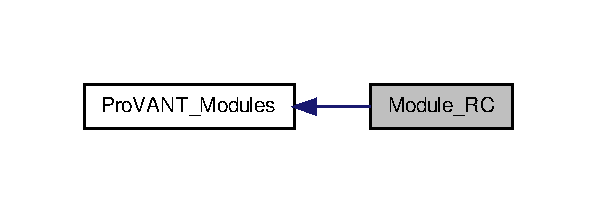
\includegraphics[width=286pt]{group__Module__RC}
\end{center}
\end{figure}
\subsection*{Macros}
\begin{DoxyCompactItemize}
\item 
\#define \hyperlink{group__Module__RC_ga0ac6c9f2991b096e49c354e5cce6fae0}{M\-O\-D\-U\-L\-E\-\_\-\-P\-E\-R\-I\-O\-D}~10
\item 
\#define \hyperlink{group__Module__RC_gaec8246e954743c1eca3ed9d0b934bf8e}{E\-S\-C\-\_\-\-O\-N}~1
\item 
\#define \hyperlink{group__Module__RC_ga162e9e4abd94f1558733bbf17fca28e9}{S\-E\-R\-V\-O\-\_\-\-O\-N}~1
\end{DoxyCompactItemize}
\subsection*{Funções}
\begin{DoxyCompactItemize}
\item 
void \hyperlink{group__Module__RC_gabedb9a5c3739466a359c93b3585a3640}{module\-\_\-co\-\_\-init} ()
\begin{DoxyCompactList}\small\item\em Inicializacao do módulo de R\-C. \end{DoxyCompactList}\item 
void \hyperlink{group__Module__RC_gaab8216fc955d01b47e3431aae288d9d3}{module\-\_\-co\-\_\-run} ()
\begin{DoxyCompactList}\small\item\em Função principal do módulo de R\-C. \end{DoxyCompactList}\end{DoxyCompactItemize}
\subsection*{Variáveis}
\begin{DoxyCompactItemize}
\item 
port\-Tick\-Type \hyperlink{group__Module__RC_gaa8db3871cb5f64abbd94ddd5a1db73a6}{last\-Wake\-Time}
\item 
pv\-\_\-msg\-\_\-input \hyperlink{group__Module__RC_gac40b8cfe5fd2000670ad57fe3e75ec89}{i\-Input\-Data}
\item 
pv\-\_\-msg\-\_\-control\-Output \hyperlink{group__Module__RC_ga0a14ca4568444d2d76c256fa91585cdf}{o\-Control\-Output\-Data}
\end{DoxyCompactItemize}


\subsection{Descrição detalhada}
Módulo com as principais funcionalidades para operação em modo rádio controlado. Definição do módulo de controle e comunicação via rádio manual. 

\subsection{Documentação das macros}
\hypertarget{group__Module__RC_gaec8246e954743c1eca3ed9d0b934bf8e}{\index{Module\-\_\-\-R\-C@{Module\-\_\-\-R\-C}!E\-S\-C\-\_\-\-O\-N@{E\-S\-C\-\_\-\-O\-N}}
\index{E\-S\-C\-\_\-\-O\-N@{E\-S\-C\-\_\-\-O\-N}!Module_RC@{Module\-\_\-\-R\-C}}
\subsubsection[{E\-S\-C\-\_\-\-O\-N}]{\setlength{\rightskip}{0pt plus 5cm}\#define E\-S\-C\-\_\-\-O\-N~1}}\label{group__Module__RC_gaec8246e954743c1eca3ed9d0b934bf8e}


Definido na linha 27 do ficheiro pv\-\_\-module\-\_\-co.\-c.

\hypertarget{group__Module__RC_ga0ac6c9f2991b096e49c354e5cce6fae0}{\index{Module\-\_\-\-R\-C@{Module\-\_\-\-R\-C}!M\-O\-D\-U\-L\-E\-\_\-\-P\-E\-R\-I\-O\-D@{M\-O\-D\-U\-L\-E\-\_\-\-P\-E\-R\-I\-O\-D}}
\index{M\-O\-D\-U\-L\-E\-\_\-\-P\-E\-R\-I\-O\-D@{M\-O\-D\-U\-L\-E\-\_\-\-P\-E\-R\-I\-O\-D}!Module_RC@{Module\-\_\-\-R\-C}}
\subsubsection[{M\-O\-D\-U\-L\-E\-\_\-\-P\-E\-R\-I\-O\-D}]{\setlength{\rightskip}{0pt plus 5cm}\#define M\-O\-D\-U\-L\-E\-\_\-\-P\-E\-R\-I\-O\-D~10}}\label{group__Module__RC_ga0ac6c9f2991b096e49c354e5cce6fae0}


Definido na linha 26 do ficheiro pv\-\_\-module\-\_\-co.\-c.

\hypertarget{group__Module__RC_ga162e9e4abd94f1558733bbf17fca28e9}{\index{Module\-\_\-\-R\-C@{Module\-\_\-\-R\-C}!S\-E\-R\-V\-O\-\_\-\-O\-N@{S\-E\-R\-V\-O\-\_\-\-O\-N}}
\index{S\-E\-R\-V\-O\-\_\-\-O\-N@{S\-E\-R\-V\-O\-\_\-\-O\-N}!Module_RC@{Module\-\_\-\-R\-C}}
\subsubsection[{S\-E\-R\-V\-O\-\_\-\-O\-N}]{\setlength{\rightskip}{0pt plus 5cm}\#define S\-E\-R\-V\-O\-\_\-\-O\-N~1}}\label{group__Module__RC_ga162e9e4abd94f1558733bbf17fca28e9}


Definido na linha 28 do ficheiro pv\-\_\-module\-\_\-co.\-c.



\subsection{Documentação das funções}
\hypertarget{group__Module__RC_gabedb9a5c3739466a359c93b3585a3640}{\index{Module\-\_\-\-R\-C@{Module\-\_\-\-R\-C}!module\-\_\-co\-\_\-init@{module\-\_\-co\-\_\-init}}
\index{module\-\_\-co\-\_\-init@{module\-\_\-co\-\_\-init}!Module_RC@{Module\-\_\-\-R\-C}}
\subsubsection[{module\-\_\-co\-\_\-init}]{\setlength{\rightskip}{0pt plus 5cm}void module\-\_\-co\-\_\-init (
\begin{DoxyParamCaption}
{}
\end{DoxyParamCaption}
)}}\label{group__Module__RC_gabedb9a5c3739466a359c93b3585a3640}


Inicializacao do módulo de R\-C. 

Instancia as Queues de comunicação inter-\/thread, inicializa a pinagem necessária para o controle remoto e aloca o que for necessário para as equações de controle. 
\begin{DoxyParams}{Parâmetros}
{\em None} & \\
\hline
\end{DoxyParams}

\begin{DoxyRetVals}{Valores retornados}
{\em None} & \\
\hline
\end{DoxyRetVals}


Definido na linha 50 do ficheiro pv\-\_\-module\-\_\-co.\-c.

\hypertarget{group__Module__RC_gaab8216fc955d01b47e3431aae288d9d3}{\index{Module\-\_\-\-R\-C@{Module\-\_\-\-R\-C}!module\-\_\-co\-\_\-run@{module\-\_\-co\-\_\-run}}
\index{module\-\_\-co\-\_\-run@{module\-\_\-co\-\_\-run}!Module_RC@{Module\-\_\-\-R\-C}}
\subsubsection[{module\-\_\-co\-\_\-run}]{\setlength{\rightskip}{0pt plus 5cm}void module\-\_\-co\-\_\-run (
\begin{DoxyParamCaption}
{}
\end{DoxyParamCaption}
)}}\label{group__Module__RC_gaab8216fc955d01b47e3431aae288d9d3}


Função principal do módulo de R\-C. 


\begin{DoxyParams}{Parâmetros}
{\em None} & \\
\hline
\end{DoxyParams}

\begin{DoxyRetVals}{Valores retornados}
{\em None} & Interpreta o recebimento de P\-P\-M, calcula sinais de controle e os envia via interface. Devido as diferenças do modelo matematica com a construção mecanica o sinal do angulo do servo direito deve ser adaptado. \\
\hline
\end{DoxyRetVals}


Definido na linha 87 do ficheiro pv\-\_\-module\-\_\-co.\-c.



\subsection{Documentação das variáveis}
\hypertarget{group__Module__RC_gac40b8cfe5fd2000670ad57fe3e75ec89}{\index{Module\-\_\-\-R\-C@{Module\-\_\-\-R\-C}!i\-Input\-Data@{i\-Input\-Data}}
\index{i\-Input\-Data@{i\-Input\-Data}!Module_RC@{Module\-\_\-\-R\-C}}
\subsubsection[{i\-Input\-Data}]{\setlength{\rightskip}{0pt plus 5cm}pv\-\_\-msg\-\_\-input i\-Input\-Data}}\label{group__Module__RC_gac40b8cfe5fd2000670ad57fe3e75ec89}


Definido na linha 33 do ficheiro pv\-\_\-module\-\_\-co.\-c.

\hypertarget{group__Module__RC_gaa8db3871cb5f64abbd94ddd5a1db73a6}{\index{Module\-\_\-\-R\-C@{Module\-\_\-\-R\-C}!last\-Wake\-Time@{last\-Wake\-Time}}
\index{last\-Wake\-Time@{last\-Wake\-Time}!Module_RC@{Module\-\_\-\-R\-C}}
\subsubsection[{last\-Wake\-Time}]{\setlength{\rightskip}{0pt plus 5cm}port\-Tick\-Type last\-Wake\-Time}}\label{group__Module__RC_gaa8db3871cb5f64abbd94ddd5a1db73a6}


Definido na linha 32 do ficheiro pv\-\_\-module\-\_\-co.\-c.

\hypertarget{group__Module__RC_ga0a14ca4568444d2d76c256fa91585cdf}{\index{Module\-\_\-\-R\-C@{Module\-\_\-\-R\-C}!o\-Control\-Output\-Data@{o\-Control\-Output\-Data}}
\index{o\-Control\-Output\-Data@{o\-Control\-Output\-Data}!Module_RC@{Module\-\_\-\-R\-C}}
\subsubsection[{o\-Control\-Output\-Data}]{\setlength{\rightskip}{0pt plus 5cm}pv\-\_\-msg\-\_\-control\-Output o\-Control\-Output\-Data}}\label{group__Module__RC_ga0a14ca4568444d2d76c256fa91585cdf}


Definido na linha 34 do ficheiro pv\-\_\-module\-\_\-co.\-c.


\hypertarget{group__ProVANT__app}{\section{Pro\-V\-A\-N\-T\-\_\-app}
\label{group__ProVANT__app}\index{Pro\-V\-A\-N\-T\-\_\-app@{Pro\-V\-A\-N\-T\-\_\-app}}
}
Diagrama de colaboração para Pro\-V\-A\-N\-T\-\_\-app\-:
\subsection*{Módulos}
\begin{DoxyCompactItemize}
\item 
\hyperlink{group__app__co}{App\-\_\-co}
\begin{DoxyCompactList}\small\item\em Módulo com as principais funcionalidades para calculo de controle e escrita de atuadores. \end{DoxyCompactList}\item 
\hyperlink{group__app__do}{App\-\_\-do}
\begin{DoxyCompactList}\small\item\em Módulo responsavel por transmitir dados. \end{DoxyCompactList}\item 
\hyperlink{group__app__gps}{App\-\_\-gps}
\begin{DoxyCompactList}\small\item\em Módulo responsavel por tratar os dados do G\-P\-S. \end{DoxyCompactList}\item 
\hyperlink{group__app__in}{App\-\_\-in}
\begin{DoxyCompactList}\small\item\em Componentes para o sensoriamento do V\-A\-N\-T. \end{DoxyCompactList}\item 
\hyperlink{group__app__sm}{App\-\_\-sm}
\begin{DoxyCompactList}\small\item\em Módulo responsavel pela maquina de estados do V\-A\-N\-T. \end{DoxyCompactList}\end{DoxyCompactItemize}


\subsection{Descrição detalhada}

\hypertarget{group__app__do}{\section{App\-\_\-do}
\label{group__app__do}\index{App\-\_\-do@{App\-\_\-do}}
}


Módulo responsavel por transmitir dados.  


Diagrama de colaboração para App\-\_\-do\-:
\nopagebreak
\begin{figure}[H]
\begin{center}
\leavevmode
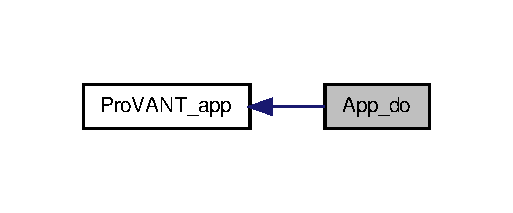
\includegraphics[width=246pt]{group__app__do}
\end{center}
\end{figure}
\subsection*{Macros}
\begin{DoxyCompactItemize}
\item 
\#define \hyperlink{group__app__do_ga0ac6c9f2991b096e49c354e5cce6fae0}{M\-O\-D\-U\-L\-E\-\_\-\-P\-E\-R\-I\-O\-D}~100
\item 
\#define \hyperlink{group__app__do_ga6a53a6c94a70cc286e300a0ea8f46ba4}{U\-S\-A\-R\-T\-\_\-\-B\-A\-U\-D\-R\-A\-T\-E}~460800
\end{DoxyCompactItemize}
\subsection*{Funções}
\begin{DoxyCompactItemize}
\item 
void \hyperlink{group__app__do_ga901c023651503207f5cfd8cdb8c305b3}{module\-\_\-do\-\_\-init} ()
\begin{DoxyCompactList}\small\item\em Inicializacao do módulo de data out. \end{DoxyCompactList}\item 
void \hyperlink{group__app__do_ga1f08b4b431624465a47f47eca0520253}{module\-\_\-do\-\_\-run} ()
\begin{DoxyCompactList}\small\item\em Função principal do módulo de data out. \end{DoxyCompactList}\end{DoxyCompactItemize}
\subsection*{Variáveis}
\begin{DoxyCompactItemize}
\item 
port\-Tick\-Type \hyperlink{group__app__do_gaa8db3871cb5f64abbd94ddd5a1db73a6}{last\-Wake\-Time}
\item 
unsigned int \hyperlink{group__app__do_ga24475be702ffcc5a6f0a5557040368ef}{heart\-Beat} =0
\item 
pv\-\_\-msg\-\_\-input \hyperlink{group__app__do_gac40b8cfe5fd2000670ad57fe3e75ec89}{i\-Input\-Data}
\item 
pv\-\_\-msg\-\_\-control\-Output \hyperlink{group__app__do_gacabca53fbaffdbf13b8e5a1c29b73bc4}{i\-Control\-Output\-Data}
\end{DoxyCompactItemize}


\subsection{Descrição detalhada}
Módulo responsavel por transmitir dados. Definição do módulo de transmissão de dados. 

\subsection{Documentação das macros}
\hypertarget{group__app__do_ga0ac6c9f2991b096e49c354e5cce6fae0}{\index{App\-\_\-do@{App\-\_\-do}!M\-O\-D\-U\-L\-E\-\_\-\-P\-E\-R\-I\-O\-D@{M\-O\-D\-U\-L\-E\-\_\-\-P\-E\-R\-I\-O\-D}}
\index{M\-O\-D\-U\-L\-E\-\_\-\-P\-E\-R\-I\-O\-D@{M\-O\-D\-U\-L\-E\-\_\-\-P\-E\-R\-I\-O\-D}!App_do@{App\-\_\-do}}
\subsubsection[{M\-O\-D\-U\-L\-E\-\_\-\-P\-E\-R\-I\-O\-D}]{\setlength{\rightskip}{0pt plus 5cm}\#define M\-O\-D\-U\-L\-E\-\_\-\-P\-E\-R\-I\-O\-D~100}}\label{group__app__do_ga0ac6c9f2991b096e49c354e5cce6fae0}


Definido na linha 26 do ficheiro pv\-\_\-module\-\_\-do.\-c.

\hypertarget{group__app__do_ga6a53a6c94a70cc286e300a0ea8f46ba4}{\index{App\-\_\-do@{App\-\_\-do}!U\-S\-A\-R\-T\-\_\-\-B\-A\-U\-D\-R\-A\-T\-E@{U\-S\-A\-R\-T\-\_\-\-B\-A\-U\-D\-R\-A\-T\-E}}
\index{U\-S\-A\-R\-T\-\_\-\-B\-A\-U\-D\-R\-A\-T\-E@{U\-S\-A\-R\-T\-\_\-\-B\-A\-U\-D\-R\-A\-T\-E}!App_do@{App\-\_\-do}}
\subsubsection[{U\-S\-A\-R\-T\-\_\-\-B\-A\-U\-D\-R\-A\-T\-E}]{\setlength{\rightskip}{0pt plus 5cm}\#define U\-S\-A\-R\-T\-\_\-\-B\-A\-U\-D\-R\-A\-T\-E~460800}}\label{group__app__do_ga6a53a6c94a70cc286e300a0ea8f46ba4}


Definido na linha 27 do ficheiro pv\-\_\-module\-\_\-do.\-c.



\subsection{Documentação das funções}
\hypertarget{group__app__do_ga901c023651503207f5cfd8cdb8c305b3}{\index{App\-\_\-do@{App\-\_\-do}!module\-\_\-do\-\_\-init@{module\-\_\-do\-\_\-init}}
\index{module\-\_\-do\-\_\-init@{module\-\_\-do\-\_\-init}!App_do@{App\-\_\-do}}
\subsubsection[{module\-\_\-do\-\_\-init}]{\setlength{\rightskip}{0pt plus 5cm}void module\-\_\-do\-\_\-init (
\begin{DoxyParamCaption}
{}
\end{DoxyParamCaption}
)}}\label{group__app__do_ga901c023651503207f5cfd8cdb8c305b3}


Inicializacao do módulo de data out. 

Instancia as Queues de comunicação inter-\/thread. 
\begin{DoxyParams}{Parâmetros}
{\em None} & \\
\hline
\end{DoxyParams}

\begin{DoxyRetVals}{Valores retornados}
{\em None} & \\
\hline
\end{DoxyRetVals}


Definido na linha 44 do ficheiro pv\-\_\-module\-\_\-do.\-c.

\hypertarget{group__app__do_ga1f08b4b431624465a47f47eca0520253}{\index{App\-\_\-do@{App\-\_\-do}!module\-\_\-do\-\_\-run@{module\-\_\-do\-\_\-run}}
\index{module\-\_\-do\-\_\-run@{module\-\_\-do\-\_\-run}!App_do@{App\-\_\-do}}
\subsubsection[{module\-\_\-do\-\_\-run}]{\setlength{\rightskip}{0pt plus 5cm}void module\-\_\-do\-\_\-run (
\begin{DoxyParamCaption}
{}
\end{DoxyParamCaption}
)}}\label{group__app__do_ga1f08b4b431624465a47f47eca0520253}


Função principal do módulo de data out. 


\begin{DoxyParams}{Parâmetros}
{\em None} & \\
\hline
\end{DoxyParams}

\begin{DoxyRetVals}{Valores retornados}
{\em None} & \\
\hline
\end{DoxyRetVals}


Definido na linha 57 do ficheiro pv\-\_\-module\-\_\-do.\-c.



\subsection{Documentação das variáveis}
\hypertarget{group__app__do_ga24475be702ffcc5a6f0a5557040368ef}{\index{App\-\_\-do@{App\-\_\-do}!heart\-Beat@{heart\-Beat}}
\index{heart\-Beat@{heart\-Beat}!App_do@{App\-\_\-do}}
\subsubsection[{heart\-Beat}]{\setlength{\rightskip}{0pt plus 5cm}unsigned int heart\-Beat =0}}\label{group__app__do_ga24475be702ffcc5a6f0a5557040368ef}


Definido na linha 31 do ficheiro pv\-\_\-module\-\_\-do.\-c.

\hypertarget{group__app__do_gacabca53fbaffdbf13b8e5a1c29b73bc4}{\index{App\-\_\-do@{App\-\_\-do}!i\-Control\-Output\-Data@{i\-Control\-Output\-Data}}
\index{i\-Control\-Output\-Data@{i\-Control\-Output\-Data}!App_do@{App\-\_\-do}}
\subsubsection[{i\-Control\-Output\-Data}]{\setlength{\rightskip}{0pt plus 5cm}pv\-\_\-msg\-\_\-control\-Output i\-Control\-Output\-Data}}\label{group__app__do_gacabca53fbaffdbf13b8e5a1c29b73bc4}


Definido na linha 33 do ficheiro pv\-\_\-module\-\_\-do.\-c.

\hypertarget{group__app__do_gac40b8cfe5fd2000670ad57fe3e75ec89}{\index{App\-\_\-do@{App\-\_\-do}!i\-Input\-Data@{i\-Input\-Data}}
\index{i\-Input\-Data@{i\-Input\-Data}!App_do@{App\-\_\-do}}
\subsubsection[{i\-Input\-Data}]{\setlength{\rightskip}{0pt plus 5cm}pv\-\_\-msg\-\_\-input i\-Input\-Data}}\label{group__app__do_gac40b8cfe5fd2000670ad57fe3e75ec89}


Definido na linha 32 do ficheiro pv\-\_\-module\-\_\-do.\-c.

\hypertarget{group__app__do_gaa8db3871cb5f64abbd94ddd5a1db73a6}{\index{App\-\_\-do@{App\-\_\-do}!last\-Wake\-Time@{last\-Wake\-Time}}
\index{last\-Wake\-Time@{last\-Wake\-Time}!App_do@{App\-\_\-do}}
\subsubsection[{last\-Wake\-Time}]{\setlength{\rightskip}{0pt plus 5cm}port\-Tick\-Type last\-Wake\-Time}}\label{group__app__do_gaa8db3871cb5f64abbd94ddd5a1db73a6}


Definido na linha 30 do ficheiro pv\-\_\-module\-\_\-do.\-c.


\hypertarget{group__app__gps}{\section{App\-\_\-gps}
\label{group__app__gps}\index{App\-\_\-gps@{App\-\_\-gps}}
}


Módulo responsavel por tratar os dados do G\-P\-S.  


Diagrama de colaboração para App\-\_\-gps\-:
\nopagebreak
\begin{figure}[H]
\begin{center}
\leavevmode
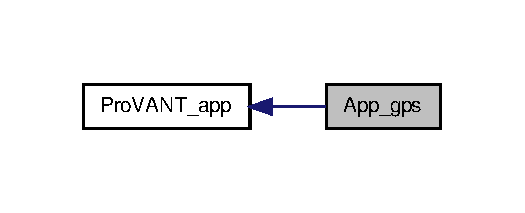
\includegraphics[width=252pt]{group__app__gps}
\end{center}
\end{figure}
\subsection*{Macros}
\begin{DoxyCompactItemize}
\item 
\#define \hyperlink{group__app__gps_ga0ac6c9f2991b096e49c354e5cce6fae0}{M\-O\-D\-U\-L\-E\-\_\-\-P\-E\-R\-I\-O\-D}~100
\end{DoxyCompactItemize}
\subsection*{Funções}
\begin{DoxyCompactItemize}
\item 
void \hyperlink{group__app__gps_ga9ee93102a0a5aec6877376bbcaf1dcb0}{module\-\_\-gps\-\_\-init} ()
\begin{DoxyCompactList}\small\item\em Inicializacao do módulo de G\-P\-S. \end{DoxyCompactList}\item 
void \hyperlink{group__app__gps_gace423457cfae0d22bd57db9e2fb4c033}{module\-\_\-gps\-\_\-run} ()
\begin{DoxyCompactList}\small\item\em Função principal do módulo de G\-P\-S. \end{DoxyCompactList}\end{DoxyCompactItemize}
\subsection*{Variáveis}
\begin{DoxyCompactItemize}
\item 
port\-Tick\-Type \hyperlink{group__app__gps_gaa8db3871cb5f64abbd94ddd5a1db73a6}{last\-Wake\-Time}
\end{DoxyCompactItemize}


\subsection{Descrição detalhada}
Módulo responsavel por tratar os dados do G\-P\-S. Definição do módulo de tratamento dos dados de G\-P\-S. 

\subsection{Documentação das macros}
\hypertarget{group__app__gps_ga0ac6c9f2991b096e49c354e5cce6fae0}{\index{App\-\_\-gps@{App\-\_\-gps}!M\-O\-D\-U\-L\-E\-\_\-\-P\-E\-R\-I\-O\-D@{M\-O\-D\-U\-L\-E\-\_\-\-P\-E\-R\-I\-O\-D}}
\index{M\-O\-D\-U\-L\-E\-\_\-\-P\-E\-R\-I\-O\-D@{M\-O\-D\-U\-L\-E\-\_\-\-P\-E\-R\-I\-O\-D}!App_gps@{App\-\_\-gps}}
\subsubsection[{M\-O\-D\-U\-L\-E\-\_\-\-P\-E\-R\-I\-O\-D}]{\setlength{\rightskip}{0pt plus 5cm}\#define M\-O\-D\-U\-L\-E\-\_\-\-P\-E\-R\-I\-O\-D~100}}\label{group__app__gps_ga0ac6c9f2991b096e49c354e5cce6fae0}


Definido na linha 26 do ficheiro pv\-\_\-module\-\_\-gps.\-c.



\subsection{Documentação das funções}
\hypertarget{group__app__gps_ga9ee93102a0a5aec6877376bbcaf1dcb0}{\index{App\-\_\-gps@{App\-\_\-gps}!module\-\_\-gps\-\_\-init@{module\-\_\-gps\-\_\-init}}
\index{module\-\_\-gps\-\_\-init@{module\-\_\-gps\-\_\-init}!App_gps@{App\-\_\-gps}}
\subsubsection[{module\-\_\-gps\-\_\-init}]{\setlength{\rightskip}{0pt plus 5cm}void module\-\_\-gps\-\_\-init (
\begin{DoxyParamCaption}
{}
\end{DoxyParamCaption}
)}}\label{group__app__gps_ga9ee93102a0a5aec6877376bbcaf1dcb0}


Inicializacao do módulo de G\-P\-S. 

Instancia as Queues de comunicação inter-\/thread. 
\begin{DoxyParams}{Parâmetros}
{\em None} & \\
\hline
\end{DoxyParams}

\begin{DoxyRetVals}{Valores retornados}
{\em None} & \\
\hline
\end{DoxyRetVals}


Definido na linha 41 do ficheiro pv\-\_\-module\-\_\-gps.\-c.

\hypertarget{group__app__gps_gace423457cfae0d22bd57db9e2fb4c033}{\index{App\-\_\-gps@{App\-\_\-gps}!module\-\_\-gps\-\_\-run@{module\-\_\-gps\-\_\-run}}
\index{module\-\_\-gps\-\_\-run@{module\-\_\-gps\-\_\-run}!App_gps@{App\-\_\-gps}}
\subsubsection[{module\-\_\-gps\-\_\-run}]{\setlength{\rightskip}{0pt plus 5cm}void module\-\_\-gps\-\_\-run (
\begin{DoxyParamCaption}
{}
\end{DoxyParamCaption}
)}}\label{group__app__gps_gace423457cfae0d22bd57db9e2fb4c033}


Função principal do módulo de G\-P\-S. 


\begin{DoxyParams}{Parâmetros}
{\em None} & \\
\hline
\end{DoxyParams}

\begin{DoxyRetVals}{Valores retornados}
{\em None} & \\
\hline
\end{DoxyRetVals}


Definido na linha 50 do ficheiro pv\-\_\-module\-\_\-gps.\-c.



\subsection{Documentação das variáveis}
\hypertarget{group__app__gps_gaa8db3871cb5f64abbd94ddd5a1db73a6}{\index{App\-\_\-gps@{App\-\_\-gps}!last\-Wake\-Time@{last\-Wake\-Time}}
\index{last\-Wake\-Time@{last\-Wake\-Time}!App_gps@{App\-\_\-gps}}
\subsubsection[{last\-Wake\-Time}]{\setlength{\rightskip}{0pt plus 5cm}port\-Tick\-Type last\-Wake\-Time}}\label{group__app__gps_gaa8db3871cb5f64abbd94ddd5a1db73a6}


Definido na linha 30 do ficheiro pv\-\_\-module\-\_\-gps.\-c.


\hypertarget{group__Module__IO}{\section{Module\-\_\-\-I\-O}
\label{group__Module__IO}\index{Module\-\_\-\-I\-O@{Module\-\_\-\-I\-O}}
}


Componentes para atuação e sensoriamento do V\-A\-N\-T.  


Diagrama de colaboração para Module\-\_\-\-I\-O\-:
\nopagebreak
\begin{figure}[H]
\begin{center}
\leavevmode
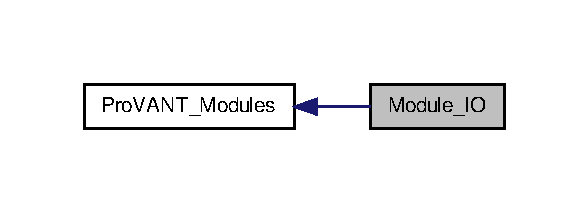
\includegraphics[width=282pt]{group__Module__IO}
\end{center}
\end{figure}
\subsection*{Macros}
\begin{DoxyCompactItemize}
\item 
\#define \hyperlink{group__Module__IO_ga0ac6c9f2991b096e49c354e5cce6fae0}{M\-O\-D\-U\-L\-E\-\_\-\-P\-E\-R\-I\-O\-D}~10
\end{DoxyCompactItemize}
\subsection*{Funções}
\begin{DoxyCompactItemize}
\item 
void \hyperlink{group__Module__IO_gaffe0980a750cbec13ebf241c933460dd}{module\-\_\-in\-\_\-init} ()
\begin{DoxyCompactList}\small\item\em Inicializacao componentes de I\-O. \end{DoxyCompactList}\item 
void \hyperlink{group__Module__IO_ga2b56089e4c5adb9ac8b7a41fc1a0b0b2}{module\-\_\-in\-\_\-run} ()
\begin{DoxyCompactList}\small\item\em Função principal do módulo de I\-O. \end{DoxyCompactList}\end{DoxyCompactItemize}
\subsection*{Variáveis}
\begin{DoxyCompactItemize}
\item 
port\-Tick\-Type \hyperlink{group__Module__IO_gaa8db3871cb5f64abbd94ddd5a1db73a6}{last\-Wake\-Time}
\item 
pv\-\_\-msg\-\_\-input \hyperlink{group__Module__IO_gaffc6f7805bab2d46af160c6f7715ba99}{o\-Input\-Data}
\end{DoxyCompactItemize}


\subsection{Descrição detalhada}
Componentes para atuação e sensoriamento do V\-A\-N\-T. Reunião de todos os componentes relacionados às operações de I/\-O do V\-A\-N\-T. Leituras de todos os sensores, comandos para atuadores. O processamento destes dados brutos NÃ\-O é feito neste módulo. 

\subsection{Documentação das macros}
\hypertarget{group__Module__IO_ga0ac6c9f2991b096e49c354e5cce6fae0}{\index{Module\-\_\-\-I\-O@{Module\-\_\-\-I\-O}!M\-O\-D\-U\-L\-E\-\_\-\-P\-E\-R\-I\-O\-D@{M\-O\-D\-U\-L\-E\-\_\-\-P\-E\-R\-I\-O\-D}}
\index{M\-O\-D\-U\-L\-E\-\_\-\-P\-E\-R\-I\-O\-D@{M\-O\-D\-U\-L\-E\-\_\-\-P\-E\-R\-I\-O\-D}!Module_IO@{Module\-\_\-\-I\-O}}
\subsubsection[{M\-O\-D\-U\-L\-E\-\_\-\-P\-E\-R\-I\-O\-D}]{\setlength{\rightskip}{0pt plus 5cm}\#define M\-O\-D\-U\-L\-E\-\_\-\-P\-E\-R\-I\-O\-D~10}}\label{group__Module__IO_ga0ac6c9f2991b096e49c354e5cce6fae0}


Definido na linha 28 do ficheiro pv\-\_\-module\-\_\-in.\-c.



\subsection{Documentação das funções}
\hypertarget{group__Module__IO_gaffe0980a750cbec13ebf241c933460dd}{\index{Module\-\_\-\-I\-O@{Module\-\_\-\-I\-O}!module\-\_\-in\-\_\-init@{module\-\_\-in\-\_\-init}}
\index{module\-\_\-in\-\_\-init@{module\-\_\-in\-\_\-init}!Module_IO@{Module\-\_\-\-I\-O}}
\subsubsection[{module\-\_\-in\-\_\-init}]{\setlength{\rightskip}{0pt plus 5cm}void module\-\_\-in\-\_\-init (
\begin{DoxyParamCaption}
{}
\end{DoxyParamCaption}
)}}\label{group__Module__IO_gaffe0980a750cbec13ebf241c933460dd}


Inicializacao componentes de I\-O. 

Incializa o hardware para comunicar com os sensores e atuadores. Rotinas de teste ainda precisam ser executadas. 
\begin{DoxyParams}{Parâmetros}
{\em None} & \\
\hline
\end{DoxyParams}

\begin{DoxyRetVals}{Valores retornados}
{\em None} & \\
\hline
\end{DoxyRetVals}


Definido na linha 45 do ficheiro pv\-\_\-module\-\_\-in.\-c.

\hypertarget{group__Module__IO_ga2b56089e4c5adb9ac8b7a41fc1a0b0b2}{\index{Module\-\_\-\-I\-O@{Module\-\_\-\-I\-O}!module\-\_\-in\-\_\-run@{module\-\_\-in\-\_\-run}}
\index{module\-\_\-in\-\_\-run@{module\-\_\-in\-\_\-run}!Module_IO@{Module\-\_\-\-I\-O}}
\subsubsection[{module\-\_\-in\-\_\-run}]{\setlength{\rightskip}{0pt plus 5cm}void module\-\_\-in\-\_\-run (
\begin{DoxyParamCaption}
{}
\end{DoxyParamCaption}
)}}\label{group__Module__IO_ga2b56089e4c5adb9ac8b7a41fc1a0b0b2}


Função principal do módulo de I\-O. 


\begin{DoxyParams}{Parâmetros}
{\em None} & \\
\hline
\end{DoxyParams}

\begin{DoxyRetVals}{Valores retornados}
{\em None} & Loop que amostra sensores e escreve nos atuadores como necessário. \\
\hline
\end{DoxyRetVals}


Definido na linha 68 do ficheiro pv\-\_\-module\-\_\-in.\-c.



\subsection{Documentação das variáveis}
\hypertarget{group__Module__IO_gaa8db3871cb5f64abbd94ddd5a1db73a6}{\index{Module\-\_\-\-I\-O@{Module\-\_\-\-I\-O}!last\-Wake\-Time@{last\-Wake\-Time}}
\index{last\-Wake\-Time@{last\-Wake\-Time}!Module_IO@{Module\-\_\-\-I\-O}}
\subsubsection[{last\-Wake\-Time}]{\setlength{\rightskip}{0pt plus 5cm}port\-Tick\-Type last\-Wake\-Time}}\label{group__Module__IO_gaa8db3871cb5f64abbd94ddd5a1db73a6}


Definido na linha 32 do ficheiro pv\-\_\-module\-\_\-in.\-c.

\hypertarget{group__Module__IO_gaffc6f7805bab2d46af160c6f7715ba99}{\index{Module\-\_\-\-I\-O@{Module\-\_\-\-I\-O}!o\-Input\-Data@{o\-Input\-Data}}
\index{o\-Input\-Data@{o\-Input\-Data}!Module_IO@{Module\-\_\-\-I\-O}}
\subsubsection[{o\-Input\-Data}]{\setlength{\rightskip}{0pt plus 5cm}pv\-\_\-msg\-\_\-input o\-Input\-Data}}\label{group__Module__IO_gaffc6f7805bab2d46af160c6f7715ba99}


Definido na linha 33 do ficheiro pv\-\_\-module\-\_\-in.\-c.


\hypertarget{group__app__sm}{\section{App\-\_\-sm}
\label{group__app__sm}\index{App\-\_\-sm@{App\-\_\-sm}}
}


Módulo responsavel pela maquina de estados do V\-A\-N\-T.  


Diagrama de colaboração para App\-\_\-sm\-:
\subsection*{Macros}
\begin{DoxyCompactItemize}
\item 
\#define \hyperlink{group__app__sm_ga0ac6c9f2991b096e49c354e5cce6fae0}{M\-O\-D\-U\-L\-E\-\_\-\-P\-E\-R\-I\-O\-D}~20
\end{DoxyCompactItemize}
\subsection*{Funções}
\begin{DoxyCompactItemize}
\item 
void \hyperlink{group__app__sm_gaf1b95b5ff451c9c5d9a4cdd34531201b}{module\-\_\-sm\-\_\-init} ()
\begin{DoxyCompactList}\small\item\em Inicializacao do módulo de sm. \end{DoxyCompactList}\item 
void \hyperlink{group__app__sm_ga81e54a060d460608697719ba6afab1e4}{module\-\_\-sm\-\_\-run} ()
\begin{DoxyCompactList}\small\item\em Função principal do módulo da sm. \end{DoxyCompactList}\end{DoxyCompactItemize}
\subsection*{Variáveis}
\begin{DoxyCompactItemize}
\item 
port\-Tick\-Type \hyperlink{group__app__sm_gaa8db3871cb5f64abbd94ddd5a1db73a6}{last\-Wake\-Time}
\end{DoxyCompactItemize}


\subsection{Descrição detalhada}
Módulo responsavel pela maquina de estados do V\-A\-N\-T. Definição do módulo da maquina de estados. 

\subsection{Documentação das macros}
\hypertarget{group__app__sm_ga0ac6c9f2991b096e49c354e5cce6fae0}{\index{App\-\_\-sm@{App\-\_\-sm}!M\-O\-D\-U\-L\-E\-\_\-\-P\-E\-R\-I\-O\-D@{M\-O\-D\-U\-L\-E\-\_\-\-P\-E\-R\-I\-O\-D}}
\index{M\-O\-D\-U\-L\-E\-\_\-\-P\-E\-R\-I\-O\-D@{M\-O\-D\-U\-L\-E\-\_\-\-P\-E\-R\-I\-O\-D}!App_sm@{App\-\_\-sm}}
\subsubsection[{M\-O\-D\-U\-L\-E\-\_\-\-P\-E\-R\-I\-O\-D}]{\setlength{\rightskip}{0pt plus 5cm}\#define M\-O\-D\-U\-L\-E\-\_\-\-P\-E\-R\-I\-O\-D~20}}\label{group__app__sm_ga0ac6c9f2991b096e49c354e5cce6fae0}


Definido na linha 26 do ficheiro pv\-\_\-module\-\_\-sm.\-c.



\subsection{Documentação das funções}
\hypertarget{group__app__sm_gaf1b95b5ff451c9c5d9a4cdd34531201b}{\index{App\-\_\-sm@{App\-\_\-sm}!module\-\_\-sm\-\_\-init@{module\-\_\-sm\-\_\-init}}
\index{module\-\_\-sm\-\_\-init@{module\-\_\-sm\-\_\-init}!App_sm@{App\-\_\-sm}}
\subsubsection[{module\-\_\-sm\-\_\-init}]{\setlength{\rightskip}{0pt plus 5cm}void module\-\_\-sm\-\_\-init (
\begin{DoxyParamCaption}
{}
\end{DoxyParamCaption}
)}}\label{group__app__sm_gaf1b95b5ff451c9c5d9a4cdd34531201b}


Inicializacao do módulo de sm. 

Instancia as Queues de comunicação inter-\/thread. 
\begin{DoxyParams}{Parâmetros}
{\em None} & \\
\hline
\end{DoxyParams}

\begin{DoxyRetVals}{Valores retornados}
{\em None} & \\
\hline
\end{DoxyRetVals}


Definido na linha 41 do ficheiro pv\-\_\-module\-\_\-sm.\-c.

\hypertarget{group__app__sm_ga81e54a060d460608697719ba6afab1e4}{\index{App\-\_\-sm@{App\-\_\-sm}!module\-\_\-sm\-\_\-run@{module\-\_\-sm\-\_\-run}}
\index{module\-\_\-sm\-\_\-run@{module\-\_\-sm\-\_\-run}!App_sm@{App\-\_\-sm}}
\subsubsection[{module\-\_\-sm\-\_\-run}]{\setlength{\rightskip}{0pt plus 5cm}void module\-\_\-sm\-\_\-run (
\begin{DoxyParamCaption}
{}
\end{DoxyParamCaption}
)}}\label{group__app__sm_ga81e54a060d460608697719ba6afab1e4}


Função principal do módulo da sm. 


\begin{DoxyParams}{Parâmetros}
{\em None} & \\
\hline
\end{DoxyParams}

\begin{DoxyRetVals}{Valores retornados}
{\em None} & \\
\hline
\end{DoxyRetVals}


Definido na linha 50 do ficheiro pv\-\_\-module\-\_\-sm.\-c.



\subsection{Documentação das variáveis}
\hypertarget{group__app__sm_gaa8db3871cb5f64abbd94ddd5a1db73a6}{\index{App\-\_\-sm@{App\-\_\-sm}!last\-Wake\-Time@{last\-Wake\-Time}}
\index{last\-Wake\-Time@{last\-Wake\-Time}!App_sm@{App\-\_\-sm}}
\subsubsection[{last\-Wake\-Time}]{\setlength{\rightskip}{0pt plus 5cm}port\-Tick\-Type last\-Wake\-Time}}\label{group__app__sm_gaa8db3871cb5f64abbd94ddd5a1db73a6}


Definido na linha 30 do ficheiro pv\-\_\-module\-\_\-sm.\-c.


\chapter{Documentação da classe}
\hypertarget{structpv__interface__co}{\section{Referência à estrutura pv\-\_\-interface\-\_\-co}
\label{structpv__interface__co}\index{pv\-\_\-interface\-\_\-co@{pv\-\_\-interface\-\_\-co}}
}


{\ttfamily \#include $<$pv\-\_\-module\-\_\-co.\-h$>$}



Diagrama de colaboração para pv\-\_\-interface\-\_\-co\-:
\nopagebreak
\begin{figure}[H]
\begin{center}
\leavevmode
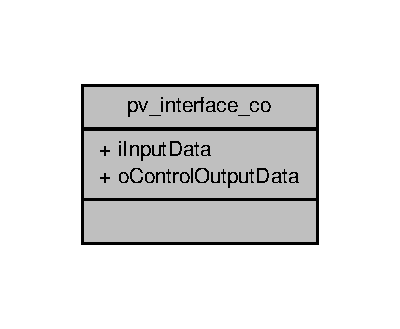
\includegraphics[width=192pt]{structpv__interface__co__coll__graph}
\end{center}
\end{figure}
\subsection*{Campos de Dados}
\begin{DoxyCompactItemize}
\item 
x\-Queue\-Handle \hyperlink{structpv__interface__co_ad057767ef15274f0933ad1821fea7239}{i\-Input\-Data}
\item 
x\-Queue\-Handle \hyperlink{structpv__interface__co_adeb92ab25c31742c709ae51f96cbf10a}{o\-Control\-Output\-Data}
\end{DoxyCompactItemize}


\subsection{Descrição detalhada}


Definido na linha 35 do ficheiro pv\-\_\-module\-\_\-co.\-h.



\subsection{Documentação dos campos e atributos}
\hypertarget{structpv__interface__co_ad057767ef15274f0933ad1821fea7239}{\index{pv\-\_\-interface\-\_\-co@{pv\-\_\-interface\-\_\-co}!i\-Input\-Data@{i\-Input\-Data}}
\index{i\-Input\-Data@{i\-Input\-Data}!pv_interface_co@{pv\-\_\-interface\-\_\-co}}
\subsubsection[{i\-Input\-Data}]{\setlength{\rightskip}{0pt plus 5cm}x\-Queue\-Handle i\-Input\-Data}}\label{structpv__interface__co_ad057767ef15274f0933ad1821fea7239}


Definido na linha 37 do ficheiro pv\-\_\-module\-\_\-co.\-h.

\hypertarget{structpv__interface__co_adeb92ab25c31742c709ae51f96cbf10a}{\index{pv\-\_\-interface\-\_\-co@{pv\-\_\-interface\-\_\-co}!o\-Control\-Output\-Data@{o\-Control\-Output\-Data}}
\index{o\-Control\-Output\-Data@{o\-Control\-Output\-Data}!pv_interface_co@{pv\-\_\-interface\-\_\-co}}
\subsubsection[{o\-Control\-Output\-Data}]{\setlength{\rightskip}{0pt plus 5cm}x\-Queue\-Handle o\-Control\-Output\-Data}}\label{structpv__interface__co_adeb92ab25c31742c709ae51f96cbf10a}


Definido na linha 38 do ficheiro pv\-\_\-module\-\_\-co.\-h.



A documentação para esta estrutura foi gerada a partir do seguinte ficheiro\-:\begin{DoxyCompactItemize}
\item 
/home/patrick/\-Desktop/git/provant-\/software/io-\/board/stm32f4/app/remote-\/controlled-\/flight/\hyperlink{pv__module__co_8h}{pv\-\_\-module\-\_\-co.\-h}\end{DoxyCompactItemize}

\hypertarget{structpv__interface__do}{\section{Referência à estrutura pv\-\_\-interface\-\_\-do}
\label{structpv__interface__do}\index{pv\-\_\-interface\-\_\-do@{pv\-\_\-interface\-\_\-do}}
}


{\ttfamily \#include $<$pv\-\_\-module\-\_\-do.\-h$>$}



Diagrama de colaboração para pv\-\_\-interface\-\_\-do\-:
\subsection*{Campos de Dados}
\begin{DoxyCompactItemize}
\item 
x\-Queue\-Handle \hyperlink{structpv__interface__do_ad057767ef15274f0933ad1821fea7239}{i\-Input\-Data}
\item 
x\-Queue\-Handle \hyperlink{structpv__interface__do_a47359dc53fe6c9e48eae67c40f5bde8a}{i\-Control\-Output\-Data}
\end{DoxyCompactItemize}


\subsection{Descrição detalhada}


Definido na linha 36 do ficheiro pv\-\_\-module\-\_\-do.\-h.



\subsection{Documentação dos campos e atributos}
\hypertarget{structpv__interface__do_a47359dc53fe6c9e48eae67c40f5bde8a}{\index{pv\-\_\-interface\-\_\-do@{pv\-\_\-interface\-\_\-do}!i\-Control\-Output\-Data@{i\-Control\-Output\-Data}}
\index{i\-Control\-Output\-Data@{i\-Control\-Output\-Data}!pv_interface_do@{pv\-\_\-interface\-\_\-do}}
\subsubsection[{i\-Control\-Output\-Data}]{\setlength{\rightskip}{0pt plus 5cm}x\-Queue\-Handle i\-Control\-Output\-Data}}\label{structpv__interface__do_a47359dc53fe6c9e48eae67c40f5bde8a}


Definido na linha 39 do ficheiro pv\-\_\-module\-\_\-do.\-h.

\hypertarget{structpv__interface__do_ad057767ef15274f0933ad1821fea7239}{\index{pv\-\_\-interface\-\_\-do@{pv\-\_\-interface\-\_\-do}!i\-Input\-Data@{i\-Input\-Data}}
\index{i\-Input\-Data@{i\-Input\-Data}!pv_interface_do@{pv\-\_\-interface\-\_\-do}}
\subsubsection[{i\-Input\-Data}]{\setlength{\rightskip}{0pt plus 5cm}x\-Queue\-Handle i\-Input\-Data}}\label{structpv__interface__do_ad057767ef15274f0933ad1821fea7239}


Definido na linha 38 do ficheiro pv\-\_\-module\-\_\-do.\-h.



A documentação para esta estrutura foi gerada a partir do seguinte ficheiro\-:\begin{DoxyCompactItemize}
\item 
/home/iuro/git/provant-\/software/io-\/board/stm32f4/app/remote-\/controlled-\/flight/\hyperlink{pv__module__do_8h}{pv\-\_\-module\-\_\-do.\-h}\end{DoxyCompactItemize}

\hypertarget{structpv__interface__in}{\section{Referência à estrutura pv\-\_\-interface\-\_\-in}
\label{structpv__interface__in}\index{pv\-\_\-interface\-\_\-in@{pv\-\_\-interface\-\_\-in}}
}


{\ttfamily \#include $<$pv\-\_\-module\-\_\-in.\-h$>$}



Diagrama de colaboração para pv\-\_\-interface\-\_\-in\-:
\subsection*{Campos de Dados}
\begin{DoxyCompactItemize}
\item 
x\-Queue\-Handle \hyperlink{structpv__interface__in_a1b28b7bd6ca96936bf91240eea51d3b9}{o\-Input\-Data}
\end{DoxyCompactItemize}


\subsection{Descrição detalhada}


Definido na linha 56 do ficheiro pv\-\_\-module\-\_\-in.\-h.



\subsection{Documentação dos campos e atributos}
\hypertarget{structpv__interface__in_a1b28b7bd6ca96936bf91240eea51d3b9}{\index{pv\-\_\-interface\-\_\-in@{pv\-\_\-interface\-\_\-in}!o\-Input\-Data@{o\-Input\-Data}}
\index{o\-Input\-Data@{o\-Input\-Data}!pv_interface_in@{pv\-\_\-interface\-\_\-in}}
\subsubsection[{o\-Input\-Data}]{\setlength{\rightskip}{0pt plus 5cm}x\-Queue\-Handle o\-Input\-Data}}\label{structpv__interface__in_a1b28b7bd6ca96936bf91240eea51d3b9}


Definido na linha 58 do ficheiro pv\-\_\-module\-\_\-in.\-h.



A documentação para esta estrutura foi gerada a partir do seguinte ficheiro\-:\begin{DoxyCompactItemize}
\item 
/home/iuro/git/provant-\/software/io-\/board/stm32f4/app/remote-\/controlled-\/flight/\hyperlink{pv__module__in_8h}{pv\-\_\-module\-\_\-in.\-h}\end{DoxyCompactItemize}

\chapter{Documentação do ficheiro}
\hypertarget{pages_8dox}{\section{Referência ao ficheiro pages.\-dox}
\label{pages_8dox}\index{pages.\-dox@{pages.\-dox}}
}

\hypertarget{setup_8dox}{\section{Referência ao ficheiro setup.\-dox}
\label{setup_8dox}\index{setup.\-dox@{setup.\-dox}}
}

\hypertarget{FreeRTOSConfig_8h}{\section{Referência ao ficheiro /home/iuro/git/provant-\/software/io-\/board/stm32f4/app/remote-\/controlled-\/flight/\-Free\-R\-T\-O\-S\-Config.h}
\label{FreeRTOSConfig_8h}\index{/home/iuro/git/provant-\/software/io-\/board/stm32f4/app/remote-\/controlled-\/flight/\-Free\-R\-T\-O\-S\-Config.\-h@{/home/iuro/git/provant-\/software/io-\/board/stm32f4/app/remote-\/controlled-\/flight/\-Free\-R\-T\-O\-S\-Config.\-h}}
}
{\ttfamily \#include \char`\"{}trc\-Kernel\-Port.\-h\char`\"{}}\\*
Diagrama de dependências de inclusão para Free\-R\-T\-O\-S\-Config.\-h\-:
\subsection*{Macros}
\begin{DoxyCompactItemize}
\item 
\#define \hyperlink{FreeRTOSConfig_8h_adde83486022745409c40605922b0bdd6}{config\-U\-S\-E\-\_\-\-P\-R\-E\-E\-M\-P\-T\-I\-O\-N}~1
\item 
\#define \hyperlink{FreeRTOSConfig_8h_ac637ae45863c19fa2e919db0ed49301f}{config\-U\-S\-E\-\_\-\-I\-D\-L\-E\-\_\-\-H\-O\-O\-K}~1
\item 
\#define \hyperlink{FreeRTOSConfig_8h_a23c5922c077106fad3f70b54d9071466}{config\-U\-S\-E\-\_\-\-T\-I\-C\-K\-\_\-\-H\-O\-O\-K}~0
\item 
\#define \hyperlink{FreeRTOSConfig_8h_aa68082df879e6fc96bcb9b26513639e7}{config\-C\-P\-U\-\_\-\-C\-L\-O\-C\-K\-\_\-\-H\-Z}~168000000
\item 
\#define \hyperlink{FreeRTOSConfig_8h_a2f0258dd1e3b877e5bc013be54c2db6a}{config\-T\-I\-C\-K\-\_\-\-R\-A\-T\-E\-\_\-\-H\-Z}~( ( port\-Tick\-Type ) 1000 )
\item 
\#define \hyperlink{FreeRTOSConfig_8h_a9a78f5ac61e6cb172dadf2a51f11db38}{config\-M\-A\-X\-\_\-\-P\-R\-I\-O\-R\-I\-T\-I\-E\-S}~( ( unsigned port\-B\-A\-S\-E\-\_\-\-T\-Y\-P\-E ) 5 )
\item 
\#define \hyperlink{FreeRTOSConfig_8h_a6c534a6cf8a00528fe0be42083484f9a}{config\-M\-I\-N\-I\-M\-A\-L\-\_\-\-S\-T\-A\-C\-K\-\_\-\-S\-I\-Z\-E}~512
\item 
\#define \hyperlink{FreeRTOSConfig_8h_a9f213227674effff0122a75d94d87938}{config\-T\-O\-T\-A\-L\-\_\-\-H\-E\-A\-P\-\_\-\-S\-I\-Z\-E}~( ( size\-\_\-t ) ( 75 $\ast$ 1024 ) )
\item 
\#define \hyperlink{FreeRTOSConfig_8h_ac388dc4041aab6997348828eb27fc1a8}{config\-M\-A\-X\-\_\-\-T\-A\-S\-K\-\_\-\-N\-A\-M\-E\-\_\-\-L\-E\-N}~( 10 )
\item 
\#define \hyperlink{FreeRTOSConfig_8h_a27f5ee137dc9f125681a31f0b0a4b3be}{config\-U\-S\-E\-\_\-\-T\-R\-A\-C\-E\-\_\-\-F\-A\-C\-I\-L\-I\-T\-Y}~1
\item 
\#define \hyperlink{FreeRTOSConfig_8h_aac311ed9b9e5ae4d2d9648b33a24acce}{config\-U\-S\-E\-\_\-16\-\_\-\-B\-I\-T\-\_\-\-T\-I\-C\-K\-S}~0
\item 
\#define \hyperlink{FreeRTOSConfig_8h_ad6a5061a742fee450ac455e4ad0f4b6c}{config\-I\-D\-L\-E\-\_\-\-S\-H\-O\-U\-L\-D\-\_\-\-Y\-I\-E\-L\-D}~1
\item 
\#define \hyperlink{FreeRTOSConfig_8h_a543bf3c79008974cc1d36bab51d94fbf}{config\-U\-S\-E\-\_\-\-M\-U\-T\-E\-X\-E\-S}~1
\item 
\#define \hyperlink{FreeRTOSConfig_8h_aa4b5138c4e42a180f0abd4f2455f90fb}{config\-Q\-U\-E\-U\-E\-\_\-\-R\-E\-G\-I\-S\-T\-R\-Y\-\_\-\-S\-I\-Z\-E}~8
\item 
\#define \hyperlink{FreeRTOSConfig_8h_a847511ee433494b1e32c90602c967ae7}{config\-C\-H\-E\-C\-K\-\_\-\-F\-O\-R\-\_\-\-S\-T\-A\-C\-K\-\_\-\-O\-V\-E\-R\-F\-L\-O\-W}~2
\item 
\#define \hyperlink{FreeRTOSConfig_8h_a9fe02d866cb1c4fbaa0c3de79f53d42d}{config\-U\-S\-E\-\_\-\-R\-E\-C\-U\-R\-S\-I\-V\-E\-\_\-\-M\-U\-T\-E\-X\-E\-S}~1
\item 
\#define \hyperlink{FreeRTOSConfig_8h_abdf48e7c9cf513f083aa9cbed0dd7cd7}{config\-U\-S\-E\-\_\-\-M\-A\-L\-L\-O\-C\-\_\-\-F\-A\-I\-L\-E\-D\-\_\-\-H\-O\-O\-K}~1
\item 
\#define \hyperlink{FreeRTOSConfig_8h_a2eb2a0baf886a7adab15b5735029434b}{config\-U\-S\-E\-\_\-\-A\-P\-P\-L\-I\-C\-A\-T\-I\-O\-N\-\_\-\-T\-A\-S\-K\-\_\-\-T\-A\-G}~0
\item 
\#define \hyperlink{FreeRTOSConfig_8h_a55778995203c57369d2fbfb10224943d}{config\-U\-S\-E\-\_\-\-C\-O\-U\-N\-T\-I\-N\-G\-\_\-\-S\-E\-M\-A\-P\-H\-O\-R\-E\-S}~1
\item 
\#define \hyperlink{FreeRTOSConfig_8h_ad8081822f3ebc7c917b63bd7bdd7bc58}{config\-G\-E\-N\-E\-R\-A\-T\-E\-\_\-\-R\-U\-N\-\_\-\-T\-I\-M\-E\-\_\-\-S\-T\-A\-T\-S}~0
\item 
\#define \hyperlink{FreeRTOSConfig_8h_a57990715eb06402474b8b47e1d562616}{config\-U\-S\-E\-\_\-\-C\-O\-\_\-\-R\-O\-U\-T\-I\-N\-E\-S}~0
\item 
\#define \hyperlink{FreeRTOSConfig_8h_ae8f3fd645e6e78dfeb8a6e874af6195a}{config\-M\-A\-X\-\_\-\-C\-O\-\_\-\-R\-O\-U\-T\-I\-N\-E\-\_\-\-P\-R\-I\-O\-R\-I\-T\-I\-E\-S}~( 2 )
\item 
\#define \hyperlink{FreeRTOSConfig_8h_ac342ae309b0c53828d2ecad3e6de355b}{config\-U\-S\-E\-\_\-\-T\-I\-M\-E\-R\-S}~1
\item 
\#define \hyperlink{FreeRTOSConfig_8h_a05c75ff9029ba3f0ab5bde9196f1e873}{config\-T\-I\-M\-E\-R\-\_\-\-T\-A\-S\-K\-\_\-\-P\-R\-I\-O\-R\-I\-T\-Y}~( 2 )
\item 
\#define \hyperlink{FreeRTOSConfig_8h_abb9aa0f31c1f3b14a15083a3c6120918}{config\-T\-I\-M\-E\-R\-\_\-\-Q\-U\-E\-U\-E\-\_\-\-L\-E\-N\-G\-T\-H}~10
\item 
\#define \hyperlink{FreeRTOSConfig_8h_aed7c7ebcdee603583a55e8ce04e55841}{config\-T\-I\-M\-E\-R\-\_\-\-T\-A\-S\-K\-\_\-\-S\-T\-A\-C\-K\-\_\-\-D\-E\-P\-T\-H}~( \hyperlink{FreeRTOSConfig_8h_a6c534a6cf8a00528fe0be42083484f9a}{config\-M\-I\-N\-I\-M\-A\-L\-\_\-\-S\-T\-A\-C\-K\-\_\-\-S\-I\-Z\-E} $\ast$ 2 )
\item 
\#define \hyperlink{FreeRTOSConfig_8h_ad6858ac8aaf726007fd19752956ef1bd}{I\-N\-C\-L\-U\-D\-E\-\_\-v\-Task\-Priority\-Set}~1
\item 
\#define \hyperlink{FreeRTOSConfig_8h_a1279eb797355460aeeec06aa524e91df}{I\-N\-C\-L\-U\-D\-E\-\_\-ux\-Task\-Priority\-Get}~1
\item 
\#define \hyperlink{FreeRTOSConfig_8h_a5ae1434fdf995108dc749ff9329f53bd}{I\-N\-C\-L\-U\-D\-E\-\_\-v\-Task\-Delete}~1
\item 
\#define \hyperlink{FreeRTOSConfig_8h_a7ee138825e57f243c8ee5fd4207b9e26}{I\-N\-C\-L\-U\-D\-E\-\_\-v\-Task\-Clean\-Up\-Resources}~1
\item 
\#define \hyperlink{FreeRTOSConfig_8h_aef8fbb97819ad3d962f334ac298206d1}{I\-N\-C\-L\-U\-D\-E\-\_\-v\-Task\-Suspend}~1
\item 
\#define \hyperlink{FreeRTOSConfig_8h_ae8459bfd5b428319bb10de9f504a53aa}{I\-N\-C\-L\-U\-D\-E\-\_\-v\-Task\-Delay\-Until}~1
\item 
\#define \hyperlink{FreeRTOSConfig_8h_a24361a6eb816a965f1ee4e2e08e364f8}{I\-N\-C\-L\-U\-D\-E\-\_\-v\-Task\-Delay}~1
\item 
\#define \hyperlink{FreeRTOSConfig_8h_a5796db11ec6f9aa38d017d2ac393c5ba}{config\-P\-R\-I\-O\-\_\-\-B\-I\-T\-S}~4        /$\ast$ 15 priority levels $\ast$/
\item 
\#define \hyperlink{FreeRTOSConfig_8h_a10da20f180ec9bd131b0052a802dbc39}{config\-L\-I\-B\-R\-A\-R\-Y\-\_\-\-L\-O\-W\-E\-S\-T\-\_\-\-I\-N\-T\-E\-R\-R\-U\-P\-T\-\_\-\-P\-R\-I\-O\-R\-I\-T\-Y}~0xf
\item 
\#define \hyperlink{FreeRTOSConfig_8h_a2254bd235d882be3061bcad0b1e8be98}{config\-L\-I\-B\-R\-A\-R\-Y\-\_\-\-M\-A\-X\-\_\-\-S\-Y\-S\-C\-A\-L\-L\-\_\-\-I\-N\-T\-E\-R\-R\-U\-P\-T\-\_\-\-P\-R\-I\-O\-R\-I\-T\-Y}~5
\item 
\#define \hyperlink{FreeRTOSConfig_8h_ac42cff506ad61d4174fa23e952e3225e}{config\-K\-E\-R\-N\-E\-L\-\_\-\-I\-N\-T\-E\-R\-R\-U\-P\-T\-\_\-\-P\-R\-I\-O\-R\-I\-T\-Y}~( \hyperlink{FreeRTOSConfig_8h_a10da20f180ec9bd131b0052a802dbc39}{config\-L\-I\-B\-R\-A\-R\-Y\-\_\-\-L\-O\-W\-E\-S\-T\-\_\-\-I\-N\-T\-E\-R\-R\-U\-P\-T\-\_\-\-P\-R\-I\-O\-R\-I\-T\-Y} $<$$<$ (8 -\/ \hyperlink{FreeRTOSConfig_8h_a5796db11ec6f9aa38d017d2ac393c5ba}{config\-P\-R\-I\-O\-\_\-\-B\-I\-T\-S}) )
\item 
\#define \hyperlink{FreeRTOSConfig_8h_a54bfc31c410ee452577a25a4552c3704}{config\-M\-A\-X\-\_\-\-S\-Y\-S\-C\-A\-L\-L\-\_\-\-I\-N\-T\-E\-R\-R\-U\-P\-T\-\_\-\-P\-R\-I\-O\-R\-I\-T\-Y}~( \hyperlink{FreeRTOSConfig_8h_a2254bd235d882be3061bcad0b1e8be98}{config\-L\-I\-B\-R\-A\-R\-Y\-\_\-\-M\-A\-X\-\_\-\-S\-Y\-S\-C\-A\-L\-L\-\_\-\-I\-N\-T\-E\-R\-R\-U\-P\-T\-\_\-\-P\-R\-I\-O\-R\-I\-T\-Y} $<$$<$ (8 -\/ \hyperlink{FreeRTOSConfig_8h_a5796db11ec6f9aa38d017d2ac393c5ba}{config\-P\-R\-I\-O\-\_\-\-B\-I\-T\-S}) )
\item 
\#define \hyperlink{FreeRTOSConfig_8h_a228c70cd48927d6ab730ed1a6dfbe35f}{config\-A\-S\-S\-E\-R\-T}(x)~if( ( x ) == 0 ) \{ task\-D\-I\-S\-A\-B\-L\-E\-\_\-\-I\-N\-T\-E\-R\-R\-U\-P\-T\-S(); for( ;; ); \}
\item 
\#define \hyperlink{FreeRTOSConfig_8h_ad43047b3ea0a146673e30637488bf754}{v\-Port\-S\-V\-C\-Handler}~S\-V\-C\-\_\-\-Handler
\item 
\#define \hyperlink{FreeRTOSConfig_8h_a6f30022da7d797dd31f1b8a11cae9a35}{x\-Port\-Pend\-S\-V\-Handler}~Pend\-S\-V\-\_\-\-Handler
\item 
\#define \hyperlink{FreeRTOSConfig_8h_ae42e6318b5d564e44f97f8c765859448}{x\-Port\-Sys\-Tick\-Handler}~Sys\-Tick\-\_\-\-Handler
\item 
\#define \hyperlink{FreeRTOSConfig_8h_a27f5ee137dc9f125681a31f0b0a4b3be}{config\-U\-S\-E\-\_\-\-T\-R\-A\-C\-E\-\_\-\-F\-A\-C\-I\-L\-I\-T\-Y}~1
\end{DoxyCompactItemize}


\subsection{Documentação das macros}
\hypertarget{FreeRTOSConfig_8h_a228c70cd48927d6ab730ed1a6dfbe35f}{\index{Free\-R\-T\-O\-S\-Config.\-h@{Free\-R\-T\-O\-S\-Config.\-h}!config\-A\-S\-S\-E\-R\-T@{config\-A\-S\-S\-E\-R\-T}}
\index{config\-A\-S\-S\-E\-R\-T@{config\-A\-S\-S\-E\-R\-T}!FreeRTOSConfig.h@{Free\-R\-T\-O\-S\-Config.\-h}}
\subsubsection[{config\-A\-S\-S\-E\-R\-T}]{\setlength{\rightskip}{0pt plus 5cm}\#define config\-A\-S\-S\-E\-R\-T(
\begin{DoxyParamCaption}
\item[{}]{x}
\end{DoxyParamCaption}
)~if( ( x ) == 0 ) \{ task\-D\-I\-S\-A\-B\-L\-E\-\_\-\-I\-N\-T\-E\-R\-R\-U\-P\-T\-S(); for( ;; ); \}}}\label{FreeRTOSConfig_8h_a228c70cd48927d6ab730ed1a6dfbe35f}


Definido na linha 155 do ficheiro Free\-R\-T\-O\-S\-Config.\-h.

\hypertarget{FreeRTOSConfig_8h_a847511ee433494b1e32c90602c967ae7}{\index{Free\-R\-T\-O\-S\-Config.\-h@{Free\-R\-T\-O\-S\-Config.\-h}!config\-C\-H\-E\-C\-K\-\_\-\-F\-O\-R\-\_\-\-S\-T\-A\-C\-K\-\_\-\-O\-V\-E\-R\-F\-L\-O\-W@{config\-C\-H\-E\-C\-K\-\_\-\-F\-O\-R\-\_\-\-S\-T\-A\-C\-K\-\_\-\-O\-V\-E\-R\-F\-L\-O\-W}}
\index{config\-C\-H\-E\-C\-K\-\_\-\-F\-O\-R\-\_\-\-S\-T\-A\-C\-K\-\_\-\-O\-V\-E\-R\-F\-L\-O\-W@{config\-C\-H\-E\-C\-K\-\_\-\-F\-O\-R\-\_\-\-S\-T\-A\-C\-K\-\_\-\-O\-V\-E\-R\-F\-L\-O\-W}!FreeRTOSConfig.h@{Free\-R\-T\-O\-S\-Config.\-h}}
\subsubsection[{config\-C\-H\-E\-C\-K\-\_\-\-F\-O\-R\-\_\-\-S\-T\-A\-C\-K\-\_\-\-O\-V\-E\-R\-F\-L\-O\-W}]{\setlength{\rightskip}{0pt plus 5cm}\#define config\-C\-H\-E\-C\-K\-\_\-\-F\-O\-R\-\_\-\-S\-T\-A\-C\-K\-\_\-\-O\-V\-E\-R\-F\-L\-O\-W~2}}\label{FreeRTOSConfig_8h_a847511ee433494b1e32c90602c967ae7}


Definido na linha 101 do ficheiro Free\-R\-T\-O\-S\-Config.\-h.

\hypertarget{FreeRTOSConfig_8h_aa68082df879e6fc96bcb9b26513639e7}{\index{Free\-R\-T\-O\-S\-Config.\-h@{Free\-R\-T\-O\-S\-Config.\-h}!config\-C\-P\-U\-\_\-\-C\-L\-O\-C\-K\-\_\-\-H\-Z@{config\-C\-P\-U\-\_\-\-C\-L\-O\-C\-K\-\_\-\-H\-Z}}
\index{config\-C\-P\-U\-\_\-\-C\-L\-O\-C\-K\-\_\-\-H\-Z@{config\-C\-P\-U\-\_\-\-C\-L\-O\-C\-K\-\_\-\-H\-Z}!FreeRTOSConfig.h@{Free\-R\-T\-O\-S\-Config.\-h}}
\subsubsection[{config\-C\-P\-U\-\_\-\-C\-L\-O\-C\-K\-\_\-\-H\-Z}]{\setlength{\rightskip}{0pt plus 5cm}\#define config\-C\-P\-U\-\_\-\-C\-L\-O\-C\-K\-\_\-\-H\-Z~168000000}}\label{FreeRTOSConfig_8h_aa68082df879e6fc96bcb9b26513639e7}


Definido na linha 90 do ficheiro Free\-R\-T\-O\-S\-Config.\-h.

\hypertarget{FreeRTOSConfig_8h_ad8081822f3ebc7c917b63bd7bdd7bc58}{\index{Free\-R\-T\-O\-S\-Config.\-h@{Free\-R\-T\-O\-S\-Config.\-h}!config\-G\-E\-N\-E\-R\-A\-T\-E\-\_\-\-R\-U\-N\-\_\-\-T\-I\-M\-E\-\_\-\-S\-T\-A\-T\-S@{config\-G\-E\-N\-E\-R\-A\-T\-E\-\_\-\-R\-U\-N\-\_\-\-T\-I\-M\-E\-\_\-\-S\-T\-A\-T\-S}}
\index{config\-G\-E\-N\-E\-R\-A\-T\-E\-\_\-\-R\-U\-N\-\_\-\-T\-I\-M\-E\-\_\-\-S\-T\-A\-T\-S@{config\-G\-E\-N\-E\-R\-A\-T\-E\-\_\-\-R\-U\-N\-\_\-\-T\-I\-M\-E\-\_\-\-S\-T\-A\-T\-S}!FreeRTOSConfig.h@{Free\-R\-T\-O\-S\-Config.\-h}}
\subsubsection[{config\-G\-E\-N\-E\-R\-A\-T\-E\-\_\-\-R\-U\-N\-\_\-\-T\-I\-M\-E\-\_\-\-S\-T\-A\-T\-S}]{\setlength{\rightskip}{0pt plus 5cm}\#define config\-G\-E\-N\-E\-R\-A\-T\-E\-\_\-\-R\-U\-N\-\_\-\-T\-I\-M\-E\-\_\-\-S\-T\-A\-T\-S~0}}\label{FreeRTOSConfig_8h_ad8081822f3ebc7c917b63bd7bdd7bc58}


Definido na linha 106 do ficheiro Free\-R\-T\-O\-S\-Config.\-h.

\hypertarget{FreeRTOSConfig_8h_ad6a5061a742fee450ac455e4ad0f4b6c}{\index{Free\-R\-T\-O\-S\-Config.\-h@{Free\-R\-T\-O\-S\-Config.\-h}!config\-I\-D\-L\-E\-\_\-\-S\-H\-O\-U\-L\-D\-\_\-\-Y\-I\-E\-L\-D@{config\-I\-D\-L\-E\-\_\-\-S\-H\-O\-U\-L\-D\-\_\-\-Y\-I\-E\-L\-D}}
\index{config\-I\-D\-L\-E\-\_\-\-S\-H\-O\-U\-L\-D\-\_\-\-Y\-I\-E\-L\-D@{config\-I\-D\-L\-E\-\_\-\-S\-H\-O\-U\-L\-D\-\_\-\-Y\-I\-E\-L\-D}!FreeRTOSConfig.h@{Free\-R\-T\-O\-S\-Config.\-h}}
\subsubsection[{config\-I\-D\-L\-E\-\_\-\-S\-H\-O\-U\-L\-D\-\_\-\-Y\-I\-E\-L\-D}]{\setlength{\rightskip}{0pt plus 5cm}\#define config\-I\-D\-L\-E\-\_\-\-S\-H\-O\-U\-L\-D\-\_\-\-Y\-I\-E\-L\-D~1}}\label{FreeRTOSConfig_8h_ad6a5061a742fee450ac455e4ad0f4b6c}


Definido na linha 98 do ficheiro Free\-R\-T\-O\-S\-Config.\-h.

\hypertarget{FreeRTOSConfig_8h_ac42cff506ad61d4174fa23e952e3225e}{\index{Free\-R\-T\-O\-S\-Config.\-h@{Free\-R\-T\-O\-S\-Config.\-h}!config\-K\-E\-R\-N\-E\-L\-\_\-\-I\-N\-T\-E\-R\-R\-U\-P\-T\-\_\-\-P\-R\-I\-O\-R\-I\-T\-Y@{config\-K\-E\-R\-N\-E\-L\-\_\-\-I\-N\-T\-E\-R\-R\-U\-P\-T\-\_\-\-P\-R\-I\-O\-R\-I\-T\-Y}}
\index{config\-K\-E\-R\-N\-E\-L\-\_\-\-I\-N\-T\-E\-R\-R\-U\-P\-T\-\_\-\-P\-R\-I\-O\-R\-I\-T\-Y@{config\-K\-E\-R\-N\-E\-L\-\_\-\-I\-N\-T\-E\-R\-R\-U\-P\-T\-\_\-\-P\-R\-I\-O\-R\-I\-T\-Y}!FreeRTOSConfig.h@{Free\-R\-T\-O\-S\-Config.\-h}}
\subsubsection[{config\-K\-E\-R\-N\-E\-L\-\_\-\-I\-N\-T\-E\-R\-R\-U\-P\-T\-\_\-\-P\-R\-I\-O\-R\-I\-T\-Y}]{\setlength{\rightskip}{0pt plus 5cm}\#define config\-K\-E\-R\-N\-E\-L\-\_\-\-I\-N\-T\-E\-R\-R\-U\-P\-T\-\_\-\-P\-R\-I\-O\-R\-I\-T\-Y~( {\bf config\-L\-I\-B\-R\-A\-R\-Y\-\_\-\-L\-O\-W\-E\-S\-T\-\_\-\-I\-N\-T\-E\-R\-R\-U\-P\-T\-\_\-\-P\-R\-I\-O\-R\-I\-T\-Y} $<$$<$ (8 -\/ {\bf config\-P\-R\-I\-O\-\_\-\-B\-I\-T\-S}) )}}\label{FreeRTOSConfig_8h_ac42cff506ad61d4174fa23e952e3225e}


Definido na linha 148 do ficheiro Free\-R\-T\-O\-S\-Config.\-h.

\hypertarget{FreeRTOSConfig_8h_a10da20f180ec9bd131b0052a802dbc39}{\index{Free\-R\-T\-O\-S\-Config.\-h@{Free\-R\-T\-O\-S\-Config.\-h}!config\-L\-I\-B\-R\-A\-R\-Y\-\_\-\-L\-O\-W\-E\-S\-T\-\_\-\-I\-N\-T\-E\-R\-R\-U\-P\-T\-\_\-\-P\-R\-I\-O\-R\-I\-T\-Y@{config\-L\-I\-B\-R\-A\-R\-Y\-\_\-\-L\-O\-W\-E\-S\-T\-\_\-\-I\-N\-T\-E\-R\-R\-U\-P\-T\-\_\-\-P\-R\-I\-O\-R\-I\-T\-Y}}
\index{config\-L\-I\-B\-R\-A\-R\-Y\-\_\-\-L\-O\-W\-E\-S\-T\-\_\-\-I\-N\-T\-E\-R\-R\-U\-P\-T\-\_\-\-P\-R\-I\-O\-R\-I\-T\-Y@{config\-L\-I\-B\-R\-A\-R\-Y\-\_\-\-L\-O\-W\-E\-S\-T\-\_\-\-I\-N\-T\-E\-R\-R\-U\-P\-T\-\_\-\-P\-R\-I\-O\-R\-I\-T\-Y}!FreeRTOSConfig.h@{Free\-R\-T\-O\-S\-Config.\-h}}
\subsubsection[{config\-L\-I\-B\-R\-A\-R\-Y\-\_\-\-L\-O\-W\-E\-S\-T\-\_\-\-I\-N\-T\-E\-R\-R\-U\-P\-T\-\_\-\-P\-R\-I\-O\-R\-I\-T\-Y}]{\setlength{\rightskip}{0pt plus 5cm}\#define config\-L\-I\-B\-R\-A\-R\-Y\-\_\-\-L\-O\-W\-E\-S\-T\-\_\-\-I\-N\-T\-E\-R\-R\-U\-P\-T\-\_\-\-P\-R\-I\-O\-R\-I\-T\-Y~0xf}}\label{FreeRTOSConfig_8h_a10da20f180ec9bd131b0052a802dbc39}


Definido na linha 138 do ficheiro Free\-R\-T\-O\-S\-Config.\-h.

\hypertarget{FreeRTOSConfig_8h_a2254bd235d882be3061bcad0b1e8be98}{\index{Free\-R\-T\-O\-S\-Config.\-h@{Free\-R\-T\-O\-S\-Config.\-h}!config\-L\-I\-B\-R\-A\-R\-Y\-\_\-\-M\-A\-X\-\_\-\-S\-Y\-S\-C\-A\-L\-L\-\_\-\-I\-N\-T\-E\-R\-R\-U\-P\-T\-\_\-\-P\-R\-I\-O\-R\-I\-T\-Y@{config\-L\-I\-B\-R\-A\-R\-Y\-\_\-\-M\-A\-X\-\_\-\-S\-Y\-S\-C\-A\-L\-L\-\_\-\-I\-N\-T\-E\-R\-R\-U\-P\-T\-\_\-\-P\-R\-I\-O\-R\-I\-T\-Y}}
\index{config\-L\-I\-B\-R\-A\-R\-Y\-\_\-\-M\-A\-X\-\_\-\-S\-Y\-S\-C\-A\-L\-L\-\_\-\-I\-N\-T\-E\-R\-R\-U\-P\-T\-\_\-\-P\-R\-I\-O\-R\-I\-T\-Y@{config\-L\-I\-B\-R\-A\-R\-Y\-\_\-\-M\-A\-X\-\_\-\-S\-Y\-S\-C\-A\-L\-L\-\_\-\-I\-N\-T\-E\-R\-R\-U\-P\-T\-\_\-\-P\-R\-I\-O\-R\-I\-T\-Y}!FreeRTOSConfig.h@{Free\-R\-T\-O\-S\-Config.\-h}}
\subsubsection[{config\-L\-I\-B\-R\-A\-R\-Y\-\_\-\-M\-A\-X\-\_\-\-S\-Y\-S\-C\-A\-L\-L\-\_\-\-I\-N\-T\-E\-R\-R\-U\-P\-T\-\_\-\-P\-R\-I\-O\-R\-I\-T\-Y}]{\setlength{\rightskip}{0pt plus 5cm}\#define config\-L\-I\-B\-R\-A\-R\-Y\-\_\-\-M\-A\-X\-\_\-\-S\-Y\-S\-C\-A\-L\-L\-\_\-\-I\-N\-T\-E\-R\-R\-U\-P\-T\-\_\-\-P\-R\-I\-O\-R\-I\-T\-Y~5}}\label{FreeRTOSConfig_8h_a2254bd235d882be3061bcad0b1e8be98}


Definido na linha 144 do ficheiro Free\-R\-T\-O\-S\-Config.\-h.

\hypertarget{FreeRTOSConfig_8h_ae8f3fd645e6e78dfeb8a6e874af6195a}{\index{Free\-R\-T\-O\-S\-Config.\-h@{Free\-R\-T\-O\-S\-Config.\-h}!config\-M\-A\-X\-\_\-\-C\-O\-\_\-\-R\-O\-U\-T\-I\-N\-E\-\_\-\-P\-R\-I\-O\-R\-I\-T\-I\-E\-S@{config\-M\-A\-X\-\_\-\-C\-O\-\_\-\-R\-O\-U\-T\-I\-N\-E\-\_\-\-P\-R\-I\-O\-R\-I\-T\-I\-E\-S}}
\index{config\-M\-A\-X\-\_\-\-C\-O\-\_\-\-R\-O\-U\-T\-I\-N\-E\-\_\-\-P\-R\-I\-O\-R\-I\-T\-I\-E\-S@{config\-M\-A\-X\-\_\-\-C\-O\-\_\-\-R\-O\-U\-T\-I\-N\-E\-\_\-\-P\-R\-I\-O\-R\-I\-T\-I\-E\-S}!FreeRTOSConfig.h@{Free\-R\-T\-O\-S\-Config.\-h}}
\subsubsection[{config\-M\-A\-X\-\_\-\-C\-O\-\_\-\-R\-O\-U\-T\-I\-N\-E\-\_\-\-P\-R\-I\-O\-R\-I\-T\-I\-E\-S}]{\setlength{\rightskip}{0pt plus 5cm}\#define config\-M\-A\-X\-\_\-\-C\-O\-\_\-\-R\-O\-U\-T\-I\-N\-E\-\_\-\-P\-R\-I\-O\-R\-I\-T\-I\-E\-S~( 2 )}}\label{FreeRTOSConfig_8h_ae8f3fd645e6e78dfeb8a6e874af6195a}


Definido na linha 110 do ficheiro Free\-R\-T\-O\-S\-Config.\-h.

\hypertarget{FreeRTOSConfig_8h_a9a78f5ac61e6cb172dadf2a51f11db38}{\index{Free\-R\-T\-O\-S\-Config.\-h@{Free\-R\-T\-O\-S\-Config.\-h}!config\-M\-A\-X\-\_\-\-P\-R\-I\-O\-R\-I\-T\-I\-E\-S@{config\-M\-A\-X\-\_\-\-P\-R\-I\-O\-R\-I\-T\-I\-E\-S}}
\index{config\-M\-A\-X\-\_\-\-P\-R\-I\-O\-R\-I\-T\-I\-E\-S@{config\-M\-A\-X\-\_\-\-P\-R\-I\-O\-R\-I\-T\-I\-E\-S}!FreeRTOSConfig.h@{Free\-R\-T\-O\-S\-Config.\-h}}
\subsubsection[{config\-M\-A\-X\-\_\-\-P\-R\-I\-O\-R\-I\-T\-I\-E\-S}]{\setlength{\rightskip}{0pt plus 5cm}\#define config\-M\-A\-X\-\_\-\-P\-R\-I\-O\-R\-I\-T\-I\-E\-S~( ( unsigned port\-B\-A\-S\-E\-\_\-\-T\-Y\-P\-E ) 5 )}}\label{FreeRTOSConfig_8h_a9a78f5ac61e6cb172dadf2a51f11db38}


Definido na linha 92 do ficheiro Free\-R\-T\-O\-S\-Config.\-h.

\hypertarget{FreeRTOSConfig_8h_a54bfc31c410ee452577a25a4552c3704}{\index{Free\-R\-T\-O\-S\-Config.\-h@{Free\-R\-T\-O\-S\-Config.\-h}!config\-M\-A\-X\-\_\-\-S\-Y\-S\-C\-A\-L\-L\-\_\-\-I\-N\-T\-E\-R\-R\-U\-P\-T\-\_\-\-P\-R\-I\-O\-R\-I\-T\-Y@{config\-M\-A\-X\-\_\-\-S\-Y\-S\-C\-A\-L\-L\-\_\-\-I\-N\-T\-E\-R\-R\-U\-P\-T\-\_\-\-P\-R\-I\-O\-R\-I\-T\-Y}}
\index{config\-M\-A\-X\-\_\-\-S\-Y\-S\-C\-A\-L\-L\-\_\-\-I\-N\-T\-E\-R\-R\-U\-P\-T\-\_\-\-P\-R\-I\-O\-R\-I\-T\-Y@{config\-M\-A\-X\-\_\-\-S\-Y\-S\-C\-A\-L\-L\-\_\-\-I\-N\-T\-E\-R\-R\-U\-P\-T\-\_\-\-P\-R\-I\-O\-R\-I\-T\-Y}!FreeRTOSConfig.h@{Free\-R\-T\-O\-S\-Config.\-h}}
\subsubsection[{config\-M\-A\-X\-\_\-\-S\-Y\-S\-C\-A\-L\-L\-\_\-\-I\-N\-T\-E\-R\-R\-U\-P\-T\-\_\-\-P\-R\-I\-O\-R\-I\-T\-Y}]{\setlength{\rightskip}{0pt plus 5cm}\#define config\-M\-A\-X\-\_\-\-S\-Y\-S\-C\-A\-L\-L\-\_\-\-I\-N\-T\-E\-R\-R\-U\-P\-T\-\_\-\-P\-R\-I\-O\-R\-I\-T\-Y~( {\bf config\-L\-I\-B\-R\-A\-R\-Y\-\_\-\-M\-A\-X\-\_\-\-S\-Y\-S\-C\-A\-L\-L\-\_\-\-I\-N\-T\-E\-R\-R\-U\-P\-T\-\_\-\-P\-R\-I\-O\-R\-I\-T\-Y} $<$$<$ (8 -\/ {\bf config\-P\-R\-I\-O\-\_\-\-B\-I\-T\-S}) )}}\label{FreeRTOSConfig_8h_a54bfc31c410ee452577a25a4552c3704}


Definido na linha 151 do ficheiro Free\-R\-T\-O\-S\-Config.\-h.

\hypertarget{FreeRTOSConfig_8h_ac388dc4041aab6997348828eb27fc1a8}{\index{Free\-R\-T\-O\-S\-Config.\-h@{Free\-R\-T\-O\-S\-Config.\-h}!config\-M\-A\-X\-\_\-\-T\-A\-S\-K\-\_\-\-N\-A\-M\-E\-\_\-\-L\-E\-N@{config\-M\-A\-X\-\_\-\-T\-A\-S\-K\-\_\-\-N\-A\-M\-E\-\_\-\-L\-E\-N}}
\index{config\-M\-A\-X\-\_\-\-T\-A\-S\-K\-\_\-\-N\-A\-M\-E\-\_\-\-L\-E\-N@{config\-M\-A\-X\-\_\-\-T\-A\-S\-K\-\_\-\-N\-A\-M\-E\-\_\-\-L\-E\-N}!FreeRTOSConfig.h@{Free\-R\-T\-O\-S\-Config.\-h}}
\subsubsection[{config\-M\-A\-X\-\_\-\-T\-A\-S\-K\-\_\-\-N\-A\-M\-E\-\_\-\-L\-E\-N}]{\setlength{\rightskip}{0pt plus 5cm}\#define config\-M\-A\-X\-\_\-\-T\-A\-S\-K\-\_\-\-N\-A\-M\-E\-\_\-\-L\-E\-N~( 10 )}}\label{FreeRTOSConfig_8h_ac388dc4041aab6997348828eb27fc1a8}


Definido na linha 95 do ficheiro Free\-R\-T\-O\-S\-Config.\-h.

\hypertarget{FreeRTOSConfig_8h_a6c534a6cf8a00528fe0be42083484f9a}{\index{Free\-R\-T\-O\-S\-Config.\-h@{Free\-R\-T\-O\-S\-Config.\-h}!config\-M\-I\-N\-I\-M\-A\-L\-\_\-\-S\-T\-A\-C\-K\-\_\-\-S\-I\-Z\-E@{config\-M\-I\-N\-I\-M\-A\-L\-\_\-\-S\-T\-A\-C\-K\-\_\-\-S\-I\-Z\-E}}
\index{config\-M\-I\-N\-I\-M\-A\-L\-\_\-\-S\-T\-A\-C\-K\-\_\-\-S\-I\-Z\-E@{config\-M\-I\-N\-I\-M\-A\-L\-\_\-\-S\-T\-A\-C\-K\-\_\-\-S\-I\-Z\-E}!FreeRTOSConfig.h@{Free\-R\-T\-O\-S\-Config.\-h}}
\subsubsection[{config\-M\-I\-N\-I\-M\-A\-L\-\_\-\-S\-T\-A\-C\-K\-\_\-\-S\-I\-Z\-E}]{\setlength{\rightskip}{0pt plus 5cm}\#define config\-M\-I\-N\-I\-M\-A\-L\-\_\-\-S\-T\-A\-C\-K\-\_\-\-S\-I\-Z\-E~512}}\label{FreeRTOSConfig_8h_a6c534a6cf8a00528fe0be42083484f9a}


Definido na linha 93 do ficheiro Free\-R\-T\-O\-S\-Config.\-h.

\hypertarget{FreeRTOSConfig_8h_a5796db11ec6f9aa38d017d2ac393c5ba}{\index{Free\-R\-T\-O\-S\-Config.\-h@{Free\-R\-T\-O\-S\-Config.\-h}!config\-P\-R\-I\-O\-\_\-\-B\-I\-T\-S@{config\-P\-R\-I\-O\-\_\-\-B\-I\-T\-S}}
\index{config\-P\-R\-I\-O\-\_\-\-B\-I\-T\-S@{config\-P\-R\-I\-O\-\_\-\-B\-I\-T\-S}!FreeRTOSConfig.h@{Free\-R\-T\-O\-S\-Config.\-h}}
\subsubsection[{config\-P\-R\-I\-O\-\_\-\-B\-I\-T\-S}]{\setlength{\rightskip}{0pt plus 5cm}\#define config\-P\-R\-I\-O\-\_\-\-B\-I\-T\-S~4        /$\ast$ 15 priority levels $\ast$/}}\label{FreeRTOSConfig_8h_a5796db11ec6f9aa38d017d2ac393c5ba}


Definido na linha 133 do ficheiro Free\-R\-T\-O\-S\-Config.\-h.

\hypertarget{FreeRTOSConfig_8h_aa4b5138c4e42a180f0abd4f2455f90fb}{\index{Free\-R\-T\-O\-S\-Config.\-h@{Free\-R\-T\-O\-S\-Config.\-h}!config\-Q\-U\-E\-U\-E\-\_\-\-R\-E\-G\-I\-S\-T\-R\-Y\-\_\-\-S\-I\-Z\-E@{config\-Q\-U\-E\-U\-E\-\_\-\-R\-E\-G\-I\-S\-T\-R\-Y\-\_\-\-S\-I\-Z\-E}}
\index{config\-Q\-U\-E\-U\-E\-\_\-\-R\-E\-G\-I\-S\-T\-R\-Y\-\_\-\-S\-I\-Z\-E@{config\-Q\-U\-E\-U\-E\-\_\-\-R\-E\-G\-I\-S\-T\-R\-Y\-\_\-\-S\-I\-Z\-E}!FreeRTOSConfig.h@{Free\-R\-T\-O\-S\-Config.\-h}}
\subsubsection[{config\-Q\-U\-E\-U\-E\-\_\-\-R\-E\-G\-I\-S\-T\-R\-Y\-\_\-\-S\-I\-Z\-E}]{\setlength{\rightskip}{0pt plus 5cm}\#define config\-Q\-U\-E\-U\-E\-\_\-\-R\-E\-G\-I\-S\-T\-R\-Y\-\_\-\-S\-I\-Z\-E~8}}\label{FreeRTOSConfig_8h_aa4b5138c4e42a180f0abd4f2455f90fb}


Definido na linha 100 do ficheiro Free\-R\-T\-O\-S\-Config.\-h.

\hypertarget{FreeRTOSConfig_8h_a2f0258dd1e3b877e5bc013be54c2db6a}{\index{Free\-R\-T\-O\-S\-Config.\-h@{Free\-R\-T\-O\-S\-Config.\-h}!config\-T\-I\-C\-K\-\_\-\-R\-A\-T\-E\-\_\-\-H\-Z@{config\-T\-I\-C\-K\-\_\-\-R\-A\-T\-E\-\_\-\-H\-Z}}
\index{config\-T\-I\-C\-K\-\_\-\-R\-A\-T\-E\-\_\-\-H\-Z@{config\-T\-I\-C\-K\-\_\-\-R\-A\-T\-E\-\_\-\-H\-Z}!FreeRTOSConfig.h@{Free\-R\-T\-O\-S\-Config.\-h}}
\subsubsection[{config\-T\-I\-C\-K\-\_\-\-R\-A\-T\-E\-\_\-\-H\-Z}]{\setlength{\rightskip}{0pt plus 5cm}\#define config\-T\-I\-C\-K\-\_\-\-R\-A\-T\-E\-\_\-\-H\-Z~( ( port\-Tick\-Type ) 1000 )}}\label{FreeRTOSConfig_8h_a2f0258dd1e3b877e5bc013be54c2db6a}


Definido na linha 91 do ficheiro Free\-R\-T\-O\-S\-Config.\-h.

\hypertarget{FreeRTOSConfig_8h_abb9aa0f31c1f3b14a15083a3c6120918}{\index{Free\-R\-T\-O\-S\-Config.\-h@{Free\-R\-T\-O\-S\-Config.\-h}!config\-T\-I\-M\-E\-R\-\_\-\-Q\-U\-E\-U\-E\-\_\-\-L\-E\-N\-G\-T\-H@{config\-T\-I\-M\-E\-R\-\_\-\-Q\-U\-E\-U\-E\-\_\-\-L\-E\-N\-G\-T\-H}}
\index{config\-T\-I\-M\-E\-R\-\_\-\-Q\-U\-E\-U\-E\-\_\-\-L\-E\-N\-G\-T\-H@{config\-T\-I\-M\-E\-R\-\_\-\-Q\-U\-E\-U\-E\-\_\-\-L\-E\-N\-G\-T\-H}!FreeRTOSConfig.h@{Free\-R\-T\-O\-S\-Config.\-h}}
\subsubsection[{config\-T\-I\-M\-E\-R\-\_\-\-Q\-U\-E\-U\-E\-\_\-\-L\-E\-N\-G\-T\-H}]{\setlength{\rightskip}{0pt plus 5cm}\#define config\-T\-I\-M\-E\-R\-\_\-\-Q\-U\-E\-U\-E\-\_\-\-L\-E\-N\-G\-T\-H~10}}\label{FreeRTOSConfig_8h_abb9aa0f31c1f3b14a15083a3c6120918}


Definido na linha 115 do ficheiro Free\-R\-T\-O\-S\-Config.\-h.

\hypertarget{FreeRTOSConfig_8h_a05c75ff9029ba3f0ab5bde9196f1e873}{\index{Free\-R\-T\-O\-S\-Config.\-h@{Free\-R\-T\-O\-S\-Config.\-h}!config\-T\-I\-M\-E\-R\-\_\-\-T\-A\-S\-K\-\_\-\-P\-R\-I\-O\-R\-I\-T\-Y@{config\-T\-I\-M\-E\-R\-\_\-\-T\-A\-S\-K\-\_\-\-P\-R\-I\-O\-R\-I\-T\-Y}}
\index{config\-T\-I\-M\-E\-R\-\_\-\-T\-A\-S\-K\-\_\-\-P\-R\-I\-O\-R\-I\-T\-Y@{config\-T\-I\-M\-E\-R\-\_\-\-T\-A\-S\-K\-\_\-\-P\-R\-I\-O\-R\-I\-T\-Y}!FreeRTOSConfig.h@{Free\-R\-T\-O\-S\-Config.\-h}}
\subsubsection[{config\-T\-I\-M\-E\-R\-\_\-\-T\-A\-S\-K\-\_\-\-P\-R\-I\-O\-R\-I\-T\-Y}]{\setlength{\rightskip}{0pt plus 5cm}\#define config\-T\-I\-M\-E\-R\-\_\-\-T\-A\-S\-K\-\_\-\-P\-R\-I\-O\-R\-I\-T\-Y~( 2 )}}\label{FreeRTOSConfig_8h_a05c75ff9029ba3f0ab5bde9196f1e873}


Definido na linha 114 do ficheiro Free\-R\-T\-O\-S\-Config.\-h.

\hypertarget{FreeRTOSConfig_8h_aed7c7ebcdee603583a55e8ce04e55841}{\index{Free\-R\-T\-O\-S\-Config.\-h@{Free\-R\-T\-O\-S\-Config.\-h}!config\-T\-I\-M\-E\-R\-\_\-\-T\-A\-S\-K\-\_\-\-S\-T\-A\-C\-K\-\_\-\-D\-E\-P\-T\-H@{config\-T\-I\-M\-E\-R\-\_\-\-T\-A\-S\-K\-\_\-\-S\-T\-A\-C\-K\-\_\-\-D\-E\-P\-T\-H}}
\index{config\-T\-I\-M\-E\-R\-\_\-\-T\-A\-S\-K\-\_\-\-S\-T\-A\-C\-K\-\_\-\-D\-E\-P\-T\-H@{config\-T\-I\-M\-E\-R\-\_\-\-T\-A\-S\-K\-\_\-\-S\-T\-A\-C\-K\-\_\-\-D\-E\-P\-T\-H}!FreeRTOSConfig.h@{Free\-R\-T\-O\-S\-Config.\-h}}
\subsubsection[{config\-T\-I\-M\-E\-R\-\_\-\-T\-A\-S\-K\-\_\-\-S\-T\-A\-C\-K\-\_\-\-D\-E\-P\-T\-H}]{\setlength{\rightskip}{0pt plus 5cm}\#define config\-T\-I\-M\-E\-R\-\_\-\-T\-A\-S\-K\-\_\-\-S\-T\-A\-C\-K\-\_\-\-D\-E\-P\-T\-H~( {\bf config\-M\-I\-N\-I\-M\-A\-L\-\_\-\-S\-T\-A\-C\-K\-\_\-\-S\-I\-Z\-E} $\ast$ 2 )}}\label{FreeRTOSConfig_8h_aed7c7ebcdee603583a55e8ce04e55841}


Definido na linha 116 do ficheiro Free\-R\-T\-O\-S\-Config.\-h.

\hypertarget{FreeRTOSConfig_8h_a9f213227674effff0122a75d94d87938}{\index{Free\-R\-T\-O\-S\-Config.\-h@{Free\-R\-T\-O\-S\-Config.\-h}!config\-T\-O\-T\-A\-L\-\_\-\-H\-E\-A\-P\-\_\-\-S\-I\-Z\-E@{config\-T\-O\-T\-A\-L\-\_\-\-H\-E\-A\-P\-\_\-\-S\-I\-Z\-E}}
\index{config\-T\-O\-T\-A\-L\-\_\-\-H\-E\-A\-P\-\_\-\-S\-I\-Z\-E@{config\-T\-O\-T\-A\-L\-\_\-\-H\-E\-A\-P\-\_\-\-S\-I\-Z\-E}!FreeRTOSConfig.h@{Free\-R\-T\-O\-S\-Config.\-h}}
\subsubsection[{config\-T\-O\-T\-A\-L\-\_\-\-H\-E\-A\-P\-\_\-\-S\-I\-Z\-E}]{\setlength{\rightskip}{0pt plus 5cm}\#define config\-T\-O\-T\-A\-L\-\_\-\-H\-E\-A\-P\-\_\-\-S\-I\-Z\-E~( ( size\-\_\-t ) ( 75 $\ast$ 1024 ) )}}\label{FreeRTOSConfig_8h_a9f213227674effff0122a75d94d87938}


Definido na linha 94 do ficheiro Free\-R\-T\-O\-S\-Config.\-h.

\hypertarget{FreeRTOSConfig_8h_aac311ed9b9e5ae4d2d9648b33a24acce}{\index{Free\-R\-T\-O\-S\-Config.\-h@{Free\-R\-T\-O\-S\-Config.\-h}!config\-U\-S\-E\-\_\-16\-\_\-\-B\-I\-T\-\_\-\-T\-I\-C\-K\-S@{config\-U\-S\-E\-\_\-16\-\_\-\-B\-I\-T\-\_\-\-T\-I\-C\-K\-S}}
\index{config\-U\-S\-E\-\_\-16\-\_\-\-B\-I\-T\-\_\-\-T\-I\-C\-K\-S@{config\-U\-S\-E\-\_\-16\-\_\-\-B\-I\-T\-\_\-\-T\-I\-C\-K\-S}!FreeRTOSConfig.h@{Free\-R\-T\-O\-S\-Config.\-h}}
\subsubsection[{config\-U\-S\-E\-\_\-16\-\_\-\-B\-I\-T\-\_\-\-T\-I\-C\-K\-S}]{\setlength{\rightskip}{0pt plus 5cm}\#define config\-U\-S\-E\-\_\-16\-\_\-\-B\-I\-T\-\_\-\-T\-I\-C\-K\-S~0}}\label{FreeRTOSConfig_8h_aac311ed9b9e5ae4d2d9648b33a24acce}


Definido na linha 97 do ficheiro Free\-R\-T\-O\-S\-Config.\-h.

\hypertarget{FreeRTOSConfig_8h_a2eb2a0baf886a7adab15b5735029434b}{\index{Free\-R\-T\-O\-S\-Config.\-h@{Free\-R\-T\-O\-S\-Config.\-h}!config\-U\-S\-E\-\_\-\-A\-P\-P\-L\-I\-C\-A\-T\-I\-O\-N\-\_\-\-T\-A\-S\-K\-\_\-\-T\-A\-G@{config\-U\-S\-E\-\_\-\-A\-P\-P\-L\-I\-C\-A\-T\-I\-O\-N\-\_\-\-T\-A\-S\-K\-\_\-\-T\-A\-G}}
\index{config\-U\-S\-E\-\_\-\-A\-P\-P\-L\-I\-C\-A\-T\-I\-O\-N\-\_\-\-T\-A\-S\-K\-\_\-\-T\-A\-G@{config\-U\-S\-E\-\_\-\-A\-P\-P\-L\-I\-C\-A\-T\-I\-O\-N\-\_\-\-T\-A\-S\-K\-\_\-\-T\-A\-G}!FreeRTOSConfig.h@{Free\-R\-T\-O\-S\-Config.\-h}}
\subsubsection[{config\-U\-S\-E\-\_\-\-A\-P\-P\-L\-I\-C\-A\-T\-I\-O\-N\-\_\-\-T\-A\-S\-K\-\_\-\-T\-A\-G}]{\setlength{\rightskip}{0pt plus 5cm}\#define config\-U\-S\-E\-\_\-\-A\-P\-P\-L\-I\-C\-A\-T\-I\-O\-N\-\_\-\-T\-A\-S\-K\-\_\-\-T\-A\-G~0}}\label{FreeRTOSConfig_8h_a2eb2a0baf886a7adab15b5735029434b}


Definido na linha 104 do ficheiro Free\-R\-T\-O\-S\-Config.\-h.

\hypertarget{FreeRTOSConfig_8h_a57990715eb06402474b8b47e1d562616}{\index{Free\-R\-T\-O\-S\-Config.\-h@{Free\-R\-T\-O\-S\-Config.\-h}!config\-U\-S\-E\-\_\-\-C\-O\-\_\-\-R\-O\-U\-T\-I\-N\-E\-S@{config\-U\-S\-E\-\_\-\-C\-O\-\_\-\-R\-O\-U\-T\-I\-N\-E\-S}}
\index{config\-U\-S\-E\-\_\-\-C\-O\-\_\-\-R\-O\-U\-T\-I\-N\-E\-S@{config\-U\-S\-E\-\_\-\-C\-O\-\_\-\-R\-O\-U\-T\-I\-N\-E\-S}!FreeRTOSConfig.h@{Free\-R\-T\-O\-S\-Config.\-h}}
\subsubsection[{config\-U\-S\-E\-\_\-\-C\-O\-\_\-\-R\-O\-U\-T\-I\-N\-E\-S}]{\setlength{\rightskip}{0pt plus 5cm}\#define config\-U\-S\-E\-\_\-\-C\-O\-\_\-\-R\-O\-U\-T\-I\-N\-E\-S~0}}\label{FreeRTOSConfig_8h_a57990715eb06402474b8b47e1d562616}


Definido na linha 109 do ficheiro Free\-R\-T\-O\-S\-Config.\-h.

\hypertarget{FreeRTOSConfig_8h_a55778995203c57369d2fbfb10224943d}{\index{Free\-R\-T\-O\-S\-Config.\-h@{Free\-R\-T\-O\-S\-Config.\-h}!config\-U\-S\-E\-\_\-\-C\-O\-U\-N\-T\-I\-N\-G\-\_\-\-S\-E\-M\-A\-P\-H\-O\-R\-E\-S@{config\-U\-S\-E\-\_\-\-C\-O\-U\-N\-T\-I\-N\-G\-\_\-\-S\-E\-M\-A\-P\-H\-O\-R\-E\-S}}
\index{config\-U\-S\-E\-\_\-\-C\-O\-U\-N\-T\-I\-N\-G\-\_\-\-S\-E\-M\-A\-P\-H\-O\-R\-E\-S@{config\-U\-S\-E\-\_\-\-C\-O\-U\-N\-T\-I\-N\-G\-\_\-\-S\-E\-M\-A\-P\-H\-O\-R\-E\-S}!FreeRTOSConfig.h@{Free\-R\-T\-O\-S\-Config.\-h}}
\subsubsection[{config\-U\-S\-E\-\_\-\-C\-O\-U\-N\-T\-I\-N\-G\-\_\-\-S\-E\-M\-A\-P\-H\-O\-R\-E\-S}]{\setlength{\rightskip}{0pt plus 5cm}\#define config\-U\-S\-E\-\_\-\-C\-O\-U\-N\-T\-I\-N\-G\-\_\-\-S\-E\-M\-A\-P\-H\-O\-R\-E\-S~1}}\label{FreeRTOSConfig_8h_a55778995203c57369d2fbfb10224943d}


Definido na linha 105 do ficheiro Free\-R\-T\-O\-S\-Config.\-h.

\hypertarget{FreeRTOSConfig_8h_ac637ae45863c19fa2e919db0ed49301f}{\index{Free\-R\-T\-O\-S\-Config.\-h@{Free\-R\-T\-O\-S\-Config.\-h}!config\-U\-S\-E\-\_\-\-I\-D\-L\-E\-\_\-\-H\-O\-O\-K@{config\-U\-S\-E\-\_\-\-I\-D\-L\-E\-\_\-\-H\-O\-O\-K}}
\index{config\-U\-S\-E\-\_\-\-I\-D\-L\-E\-\_\-\-H\-O\-O\-K@{config\-U\-S\-E\-\_\-\-I\-D\-L\-E\-\_\-\-H\-O\-O\-K}!FreeRTOSConfig.h@{Free\-R\-T\-O\-S\-Config.\-h}}
\subsubsection[{config\-U\-S\-E\-\_\-\-I\-D\-L\-E\-\_\-\-H\-O\-O\-K}]{\setlength{\rightskip}{0pt plus 5cm}\#define config\-U\-S\-E\-\_\-\-I\-D\-L\-E\-\_\-\-H\-O\-O\-K~1}}\label{FreeRTOSConfig_8h_ac637ae45863c19fa2e919db0ed49301f}


Definido na linha 88 do ficheiro Free\-R\-T\-O\-S\-Config.\-h.

\hypertarget{FreeRTOSConfig_8h_abdf48e7c9cf513f083aa9cbed0dd7cd7}{\index{Free\-R\-T\-O\-S\-Config.\-h@{Free\-R\-T\-O\-S\-Config.\-h}!config\-U\-S\-E\-\_\-\-M\-A\-L\-L\-O\-C\-\_\-\-F\-A\-I\-L\-E\-D\-\_\-\-H\-O\-O\-K@{config\-U\-S\-E\-\_\-\-M\-A\-L\-L\-O\-C\-\_\-\-F\-A\-I\-L\-E\-D\-\_\-\-H\-O\-O\-K}}
\index{config\-U\-S\-E\-\_\-\-M\-A\-L\-L\-O\-C\-\_\-\-F\-A\-I\-L\-E\-D\-\_\-\-H\-O\-O\-K@{config\-U\-S\-E\-\_\-\-M\-A\-L\-L\-O\-C\-\_\-\-F\-A\-I\-L\-E\-D\-\_\-\-H\-O\-O\-K}!FreeRTOSConfig.h@{Free\-R\-T\-O\-S\-Config.\-h}}
\subsubsection[{config\-U\-S\-E\-\_\-\-M\-A\-L\-L\-O\-C\-\_\-\-F\-A\-I\-L\-E\-D\-\_\-\-H\-O\-O\-K}]{\setlength{\rightskip}{0pt plus 5cm}\#define config\-U\-S\-E\-\_\-\-M\-A\-L\-L\-O\-C\-\_\-\-F\-A\-I\-L\-E\-D\-\_\-\-H\-O\-O\-K~1}}\label{FreeRTOSConfig_8h_abdf48e7c9cf513f083aa9cbed0dd7cd7}


Definido na linha 103 do ficheiro Free\-R\-T\-O\-S\-Config.\-h.

\hypertarget{FreeRTOSConfig_8h_a543bf3c79008974cc1d36bab51d94fbf}{\index{Free\-R\-T\-O\-S\-Config.\-h@{Free\-R\-T\-O\-S\-Config.\-h}!config\-U\-S\-E\-\_\-\-M\-U\-T\-E\-X\-E\-S@{config\-U\-S\-E\-\_\-\-M\-U\-T\-E\-X\-E\-S}}
\index{config\-U\-S\-E\-\_\-\-M\-U\-T\-E\-X\-E\-S@{config\-U\-S\-E\-\_\-\-M\-U\-T\-E\-X\-E\-S}!FreeRTOSConfig.h@{Free\-R\-T\-O\-S\-Config.\-h}}
\subsubsection[{config\-U\-S\-E\-\_\-\-M\-U\-T\-E\-X\-E\-S}]{\setlength{\rightskip}{0pt plus 5cm}\#define config\-U\-S\-E\-\_\-\-M\-U\-T\-E\-X\-E\-S~1}}\label{FreeRTOSConfig_8h_a543bf3c79008974cc1d36bab51d94fbf}


Definido na linha 99 do ficheiro Free\-R\-T\-O\-S\-Config.\-h.

\hypertarget{FreeRTOSConfig_8h_adde83486022745409c40605922b0bdd6}{\index{Free\-R\-T\-O\-S\-Config.\-h@{Free\-R\-T\-O\-S\-Config.\-h}!config\-U\-S\-E\-\_\-\-P\-R\-E\-E\-M\-P\-T\-I\-O\-N@{config\-U\-S\-E\-\_\-\-P\-R\-E\-E\-M\-P\-T\-I\-O\-N}}
\index{config\-U\-S\-E\-\_\-\-P\-R\-E\-E\-M\-P\-T\-I\-O\-N@{config\-U\-S\-E\-\_\-\-P\-R\-E\-E\-M\-P\-T\-I\-O\-N}!FreeRTOSConfig.h@{Free\-R\-T\-O\-S\-Config.\-h}}
\subsubsection[{config\-U\-S\-E\-\_\-\-P\-R\-E\-E\-M\-P\-T\-I\-O\-N}]{\setlength{\rightskip}{0pt plus 5cm}\#define config\-U\-S\-E\-\_\-\-P\-R\-E\-E\-M\-P\-T\-I\-O\-N~1}}\label{FreeRTOSConfig_8h_adde83486022745409c40605922b0bdd6}


Definido na linha 87 do ficheiro Free\-R\-T\-O\-S\-Config.\-h.

\hypertarget{FreeRTOSConfig_8h_a9fe02d866cb1c4fbaa0c3de79f53d42d}{\index{Free\-R\-T\-O\-S\-Config.\-h@{Free\-R\-T\-O\-S\-Config.\-h}!config\-U\-S\-E\-\_\-\-R\-E\-C\-U\-R\-S\-I\-V\-E\-\_\-\-M\-U\-T\-E\-X\-E\-S@{config\-U\-S\-E\-\_\-\-R\-E\-C\-U\-R\-S\-I\-V\-E\-\_\-\-M\-U\-T\-E\-X\-E\-S}}
\index{config\-U\-S\-E\-\_\-\-R\-E\-C\-U\-R\-S\-I\-V\-E\-\_\-\-M\-U\-T\-E\-X\-E\-S@{config\-U\-S\-E\-\_\-\-R\-E\-C\-U\-R\-S\-I\-V\-E\-\_\-\-M\-U\-T\-E\-X\-E\-S}!FreeRTOSConfig.h@{Free\-R\-T\-O\-S\-Config.\-h}}
\subsubsection[{config\-U\-S\-E\-\_\-\-R\-E\-C\-U\-R\-S\-I\-V\-E\-\_\-\-M\-U\-T\-E\-X\-E\-S}]{\setlength{\rightskip}{0pt plus 5cm}\#define config\-U\-S\-E\-\_\-\-R\-E\-C\-U\-R\-S\-I\-V\-E\-\_\-\-M\-U\-T\-E\-X\-E\-S~1}}\label{FreeRTOSConfig_8h_a9fe02d866cb1c4fbaa0c3de79f53d42d}


Definido na linha 102 do ficheiro Free\-R\-T\-O\-S\-Config.\-h.

\hypertarget{FreeRTOSConfig_8h_a23c5922c077106fad3f70b54d9071466}{\index{Free\-R\-T\-O\-S\-Config.\-h@{Free\-R\-T\-O\-S\-Config.\-h}!config\-U\-S\-E\-\_\-\-T\-I\-C\-K\-\_\-\-H\-O\-O\-K@{config\-U\-S\-E\-\_\-\-T\-I\-C\-K\-\_\-\-H\-O\-O\-K}}
\index{config\-U\-S\-E\-\_\-\-T\-I\-C\-K\-\_\-\-H\-O\-O\-K@{config\-U\-S\-E\-\_\-\-T\-I\-C\-K\-\_\-\-H\-O\-O\-K}!FreeRTOSConfig.h@{Free\-R\-T\-O\-S\-Config.\-h}}
\subsubsection[{config\-U\-S\-E\-\_\-\-T\-I\-C\-K\-\_\-\-H\-O\-O\-K}]{\setlength{\rightskip}{0pt plus 5cm}\#define config\-U\-S\-E\-\_\-\-T\-I\-C\-K\-\_\-\-H\-O\-O\-K~0}}\label{FreeRTOSConfig_8h_a23c5922c077106fad3f70b54d9071466}


Definido na linha 89 do ficheiro Free\-R\-T\-O\-S\-Config.\-h.

\hypertarget{FreeRTOSConfig_8h_ac342ae309b0c53828d2ecad3e6de355b}{\index{Free\-R\-T\-O\-S\-Config.\-h@{Free\-R\-T\-O\-S\-Config.\-h}!config\-U\-S\-E\-\_\-\-T\-I\-M\-E\-R\-S@{config\-U\-S\-E\-\_\-\-T\-I\-M\-E\-R\-S}}
\index{config\-U\-S\-E\-\_\-\-T\-I\-M\-E\-R\-S@{config\-U\-S\-E\-\_\-\-T\-I\-M\-E\-R\-S}!FreeRTOSConfig.h@{Free\-R\-T\-O\-S\-Config.\-h}}
\subsubsection[{config\-U\-S\-E\-\_\-\-T\-I\-M\-E\-R\-S}]{\setlength{\rightskip}{0pt plus 5cm}\#define config\-U\-S\-E\-\_\-\-T\-I\-M\-E\-R\-S~1}}\label{FreeRTOSConfig_8h_ac342ae309b0c53828d2ecad3e6de355b}


Definido na linha 113 do ficheiro Free\-R\-T\-O\-S\-Config.\-h.

\hypertarget{FreeRTOSConfig_8h_a27f5ee137dc9f125681a31f0b0a4b3be}{\index{Free\-R\-T\-O\-S\-Config.\-h@{Free\-R\-T\-O\-S\-Config.\-h}!config\-U\-S\-E\-\_\-\-T\-R\-A\-C\-E\-\_\-\-F\-A\-C\-I\-L\-I\-T\-Y@{config\-U\-S\-E\-\_\-\-T\-R\-A\-C\-E\-\_\-\-F\-A\-C\-I\-L\-I\-T\-Y}}
\index{config\-U\-S\-E\-\_\-\-T\-R\-A\-C\-E\-\_\-\-F\-A\-C\-I\-L\-I\-T\-Y@{config\-U\-S\-E\-\_\-\-T\-R\-A\-C\-E\-\_\-\-F\-A\-C\-I\-L\-I\-T\-Y}!FreeRTOSConfig.h@{Free\-R\-T\-O\-S\-Config.\-h}}
\subsubsection[{config\-U\-S\-E\-\_\-\-T\-R\-A\-C\-E\-\_\-\-F\-A\-C\-I\-L\-I\-T\-Y}]{\setlength{\rightskip}{0pt plus 5cm}\#define config\-U\-S\-E\-\_\-\-T\-R\-A\-C\-E\-\_\-\-F\-A\-C\-I\-L\-I\-T\-Y~1}}\label{FreeRTOSConfig_8h_a27f5ee137dc9f125681a31f0b0a4b3be}


Definido na linha 165 do ficheiro Free\-R\-T\-O\-S\-Config.\-h.

\hypertarget{FreeRTOSConfig_8h_a27f5ee137dc9f125681a31f0b0a4b3be}{\index{Free\-R\-T\-O\-S\-Config.\-h@{Free\-R\-T\-O\-S\-Config.\-h}!config\-U\-S\-E\-\_\-\-T\-R\-A\-C\-E\-\_\-\-F\-A\-C\-I\-L\-I\-T\-Y@{config\-U\-S\-E\-\_\-\-T\-R\-A\-C\-E\-\_\-\-F\-A\-C\-I\-L\-I\-T\-Y}}
\index{config\-U\-S\-E\-\_\-\-T\-R\-A\-C\-E\-\_\-\-F\-A\-C\-I\-L\-I\-T\-Y@{config\-U\-S\-E\-\_\-\-T\-R\-A\-C\-E\-\_\-\-F\-A\-C\-I\-L\-I\-T\-Y}!FreeRTOSConfig.h@{Free\-R\-T\-O\-S\-Config.\-h}}
\subsubsection[{config\-U\-S\-E\-\_\-\-T\-R\-A\-C\-E\-\_\-\-F\-A\-C\-I\-L\-I\-T\-Y}]{\setlength{\rightskip}{0pt plus 5cm}\#define config\-U\-S\-E\-\_\-\-T\-R\-A\-C\-E\-\_\-\-F\-A\-C\-I\-L\-I\-T\-Y~1}}\label{FreeRTOSConfig_8h_a27f5ee137dc9f125681a31f0b0a4b3be}


Definido na linha 165 do ficheiro Free\-R\-T\-O\-S\-Config.\-h.

\hypertarget{FreeRTOSConfig_8h_a1279eb797355460aeeec06aa524e91df}{\index{Free\-R\-T\-O\-S\-Config.\-h@{Free\-R\-T\-O\-S\-Config.\-h}!I\-N\-C\-L\-U\-D\-E\-\_\-ux\-Task\-Priority\-Get@{I\-N\-C\-L\-U\-D\-E\-\_\-ux\-Task\-Priority\-Get}}
\index{I\-N\-C\-L\-U\-D\-E\-\_\-ux\-Task\-Priority\-Get@{I\-N\-C\-L\-U\-D\-E\-\_\-ux\-Task\-Priority\-Get}!FreeRTOSConfig.h@{Free\-R\-T\-O\-S\-Config.\-h}}
\subsubsection[{I\-N\-C\-L\-U\-D\-E\-\_\-ux\-Task\-Priority\-Get}]{\setlength{\rightskip}{0pt plus 5cm}\#define I\-N\-C\-L\-U\-D\-E\-\_\-ux\-Task\-Priority\-Get~1}}\label{FreeRTOSConfig_8h_a1279eb797355460aeeec06aa524e91df}


Definido na linha 121 do ficheiro Free\-R\-T\-O\-S\-Config.\-h.

\hypertarget{FreeRTOSConfig_8h_a7ee138825e57f243c8ee5fd4207b9e26}{\index{Free\-R\-T\-O\-S\-Config.\-h@{Free\-R\-T\-O\-S\-Config.\-h}!I\-N\-C\-L\-U\-D\-E\-\_\-v\-Task\-Clean\-Up\-Resources@{I\-N\-C\-L\-U\-D\-E\-\_\-v\-Task\-Clean\-Up\-Resources}}
\index{I\-N\-C\-L\-U\-D\-E\-\_\-v\-Task\-Clean\-Up\-Resources@{I\-N\-C\-L\-U\-D\-E\-\_\-v\-Task\-Clean\-Up\-Resources}!FreeRTOSConfig.h@{Free\-R\-T\-O\-S\-Config.\-h}}
\subsubsection[{I\-N\-C\-L\-U\-D\-E\-\_\-v\-Task\-Clean\-Up\-Resources}]{\setlength{\rightskip}{0pt plus 5cm}\#define I\-N\-C\-L\-U\-D\-E\-\_\-v\-Task\-Clean\-Up\-Resources~1}}\label{FreeRTOSConfig_8h_a7ee138825e57f243c8ee5fd4207b9e26}


Definido na linha 123 do ficheiro Free\-R\-T\-O\-S\-Config.\-h.

\hypertarget{FreeRTOSConfig_8h_a24361a6eb816a965f1ee4e2e08e364f8}{\index{Free\-R\-T\-O\-S\-Config.\-h@{Free\-R\-T\-O\-S\-Config.\-h}!I\-N\-C\-L\-U\-D\-E\-\_\-v\-Task\-Delay@{I\-N\-C\-L\-U\-D\-E\-\_\-v\-Task\-Delay}}
\index{I\-N\-C\-L\-U\-D\-E\-\_\-v\-Task\-Delay@{I\-N\-C\-L\-U\-D\-E\-\_\-v\-Task\-Delay}!FreeRTOSConfig.h@{Free\-R\-T\-O\-S\-Config.\-h}}
\subsubsection[{I\-N\-C\-L\-U\-D\-E\-\_\-v\-Task\-Delay}]{\setlength{\rightskip}{0pt plus 5cm}\#define I\-N\-C\-L\-U\-D\-E\-\_\-v\-Task\-Delay~1}}\label{FreeRTOSConfig_8h_a24361a6eb816a965f1ee4e2e08e364f8}


Definido na linha 126 do ficheiro Free\-R\-T\-O\-S\-Config.\-h.

\hypertarget{FreeRTOSConfig_8h_ae8459bfd5b428319bb10de9f504a53aa}{\index{Free\-R\-T\-O\-S\-Config.\-h@{Free\-R\-T\-O\-S\-Config.\-h}!I\-N\-C\-L\-U\-D\-E\-\_\-v\-Task\-Delay\-Until@{I\-N\-C\-L\-U\-D\-E\-\_\-v\-Task\-Delay\-Until}}
\index{I\-N\-C\-L\-U\-D\-E\-\_\-v\-Task\-Delay\-Until@{I\-N\-C\-L\-U\-D\-E\-\_\-v\-Task\-Delay\-Until}!FreeRTOSConfig.h@{Free\-R\-T\-O\-S\-Config.\-h}}
\subsubsection[{I\-N\-C\-L\-U\-D\-E\-\_\-v\-Task\-Delay\-Until}]{\setlength{\rightskip}{0pt plus 5cm}\#define I\-N\-C\-L\-U\-D\-E\-\_\-v\-Task\-Delay\-Until~1}}\label{FreeRTOSConfig_8h_ae8459bfd5b428319bb10de9f504a53aa}


Definido na linha 125 do ficheiro Free\-R\-T\-O\-S\-Config.\-h.

\hypertarget{FreeRTOSConfig_8h_a5ae1434fdf995108dc749ff9329f53bd}{\index{Free\-R\-T\-O\-S\-Config.\-h@{Free\-R\-T\-O\-S\-Config.\-h}!I\-N\-C\-L\-U\-D\-E\-\_\-v\-Task\-Delete@{I\-N\-C\-L\-U\-D\-E\-\_\-v\-Task\-Delete}}
\index{I\-N\-C\-L\-U\-D\-E\-\_\-v\-Task\-Delete@{I\-N\-C\-L\-U\-D\-E\-\_\-v\-Task\-Delete}!FreeRTOSConfig.h@{Free\-R\-T\-O\-S\-Config.\-h}}
\subsubsection[{I\-N\-C\-L\-U\-D\-E\-\_\-v\-Task\-Delete}]{\setlength{\rightskip}{0pt plus 5cm}\#define I\-N\-C\-L\-U\-D\-E\-\_\-v\-Task\-Delete~1}}\label{FreeRTOSConfig_8h_a5ae1434fdf995108dc749ff9329f53bd}


Definido na linha 122 do ficheiro Free\-R\-T\-O\-S\-Config.\-h.

\hypertarget{FreeRTOSConfig_8h_ad6858ac8aaf726007fd19752956ef1bd}{\index{Free\-R\-T\-O\-S\-Config.\-h@{Free\-R\-T\-O\-S\-Config.\-h}!I\-N\-C\-L\-U\-D\-E\-\_\-v\-Task\-Priority\-Set@{I\-N\-C\-L\-U\-D\-E\-\_\-v\-Task\-Priority\-Set}}
\index{I\-N\-C\-L\-U\-D\-E\-\_\-v\-Task\-Priority\-Set@{I\-N\-C\-L\-U\-D\-E\-\_\-v\-Task\-Priority\-Set}!FreeRTOSConfig.h@{Free\-R\-T\-O\-S\-Config.\-h}}
\subsubsection[{I\-N\-C\-L\-U\-D\-E\-\_\-v\-Task\-Priority\-Set}]{\setlength{\rightskip}{0pt plus 5cm}\#define I\-N\-C\-L\-U\-D\-E\-\_\-v\-Task\-Priority\-Set~1}}\label{FreeRTOSConfig_8h_ad6858ac8aaf726007fd19752956ef1bd}


Definido na linha 120 do ficheiro Free\-R\-T\-O\-S\-Config.\-h.

\hypertarget{FreeRTOSConfig_8h_aef8fbb97819ad3d962f334ac298206d1}{\index{Free\-R\-T\-O\-S\-Config.\-h@{Free\-R\-T\-O\-S\-Config.\-h}!I\-N\-C\-L\-U\-D\-E\-\_\-v\-Task\-Suspend@{I\-N\-C\-L\-U\-D\-E\-\_\-v\-Task\-Suspend}}
\index{I\-N\-C\-L\-U\-D\-E\-\_\-v\-Task\-Suspend@{I\-N\-C\-L\-U\-D\-E\-\_\-v\-Task\-Suspend}!FreeRTOSConfig.h@{Free\-R\-T\-O\-S\-Config.\-h}}
\subsubsection[{I\-N\-C\-L\-U\-D\-E\-\_\-v\-Task\-Suspend}]{\setlength{\rightskip}{0pt plus 5cm}\#define I\-N\-C\-L\-U\-D\-E\-\_\-v\-Task\-Suspend~1}}\label{FreeRTOSConfig_8h_aef8fbb97819ad3d962f334ac298206d1}


Definido na linha 124 do ficheiro Free\-R\-T\-O\-S\-Config.\-h.

\hypertarget{FreeRTOSConfig_8h_ad43047b3ea0a146673e30637488bf754}{\index{Free\-R\-T\-O\-S\-Config.\-h@{Free\-R\-T\-O\-S\-Config.\-h}!v\-Port\-S\-V\-C\-Handler@{v\-Port\-S\-V\-C\-Handler}}
\index{v\-Port\-S\-V\-C\-Handler@{v\-Port\-S\-V\-C\-Handler}!FreeRTOSConfig.h@{Free\-R\-T\-O\-S\-Config.\-h}}
\subsubsection[{v\-Port\-S\-V\-C\-Handler}]{\setlength{\rightskip}{0pt plus 5cm}\#define v\-Port\-S\-V\-C\-Handler~S\-V\-C\-\_\-\-Handler}}\label{FreeRTOSConfig_8h_ad43047b3ea0a146673e30637488bf754}


Definido na linha 159 do ficheiro Free\-R\-T\-O\-S\-Config.\-h.

\hypertarget{FreeRTOSConfig_8h_a6f30022da7d797dd31f1b8a11cae9a35}{\index{Free\-R\-T\-O\-S\-Config.\-h@{Free\-R\-T\-O\-S\-Config.\-h}!x\-Port\-Pend\-S\-V\-Handler@{x\-Port\-Pend\-S\-V\-Handler}}
\index{x\-Port\-Pend\-S\-V\-Handler@{x\-Port\-Pend\-S\-V\-Handler}!FreeRTOSConfig.h@{Free\-R\-T\-O\-S\-Config.\-h}}
\subsubsection[{x\-Port\-Pend\-S\-V\-Handler}]{\setlength{\rightskip}{0pt plus 5cm}\#define x\-Port\-Pend\-S\-V\-Handler~Pend\-S\-V\-\_\-\-Handler}}\label{FreeRTOSConfig_8h_a6f30022da7d797dd31f1b8a11cae9a35}


Definido na linha 160 do ficheiro Free\-R\-T\-O\-S\-Config.\-h.

\hypertarget{FreeRTOSConfig_8h_ae42e6318b5d564e44f97f8c765859448}{\index{Free\-R\-T\-O\-S\-Config.\-h@{Free\-R\-T\-O\-S\-Config.\-h}!x\-Port\-Sys\-Tick\-Handler@{x\-Port\-Sys\-Tick\-Handler}}
\index{x\-Port\-Sys\-Tick\-Handler@{x\-Port\-Sys\-Tick\-Handler}!FreeRTOSConfig.h@{Free\-R\-T\-O\-S\-Config.\-h}}
\subsubsection[{x\-Port\-Sys\-Tick\-Handler}]{\setlength{\rightskip}{0pt plus 5cm}\#define x\-Port\-Sys\-Tick\-Handler~Sys\-Tick\-\_\-\-Handler}}\label{FreeRTOSConfig_8h_ae42e6318b5d564e44f97f8c765859448}


Definido na linha 161 do ficheiro Free\-R\-T\-O\-S\-Config.\-h.


\hypertarget{main_8c}{\section{Referência ao ficheiro /home/patrick/\-Desktop/git/provant-\/software/io-\/board/stm32f4/app/remote-\/controlled-\/flight/main.c}
\label{main_8c}\index{/home/patrick/\-Desktop/git/provant-\/software/io-\/board/stm32f4/app/remote-\/controlled-\/flight/main.\-c@{/home/patrick/\-Desktop/git/provant-\/software/io-\/board/stm32f4/app/remote-\/controlled-\/flight/main.\-c}}
}


Startup do projeto.  


{\ttfamily \#include $<$stdio.\-h$>$}\\*
{\ttfamily \#include $<$math.\-h$>$}\\*
{\ttfamily \#include \char`\"{}inttypes.\-h\char`\"{}}\\*
{\ttfamily \#include \char`\"{}stm32f4xx\-\_\-conf.\-h\char`\"{}}\\*
{\ttfamily \#include \char`\"{}system\-\_\-stm32f4xx.\-h\char`\"{}}\\*
{\ttfamily \#include \char`\"{}arm\-\_\-math.\-h\char`\"{}}\\*
{\ttfamily \#include \char`\"{}Free\-R\-T\-O\-S.\-h\char`\"{}}\\*
{\ttfamily \#include \char`\"{}queue.\-h\char`\"{}}\\*
{\ttfamily \#include \char`\"{}timers.\-h\char`\"{}}\\*
{\ttfamily \#include \char`\"{}task.\-h\char`\"{}}\\*
{\ttfamily \#include \char`\"{}trc\-User.\-h\char`\"{}}\\*
{\ttfamily \#include \char`\"{}pv\-\_\-module\-\_\-co.\-h\char`\"{}}\\*
{\ttfamily \#include \char`\"{}pv\-\_\-module\-\_\-in.\-h\char`\"{}}\\*
{\ttfamily \#include \char`\"{}pv\-\_\-module\-\_\-do.\-h\char`\"{}}\\*
{\ttfamily \#include \char`\"{}pv\-\_\-module\-\_\-gps.\-h\char`\"{}}\\*
{\ttfamily \#include \char`\"{}pv\-\_\-module\-\_\-sm.\-h\char`\"{}}\\*
{\ttfamily \#include \char`\"{}c\-\_\-common\-\_\-gpio.\-h\char`\"{}}\\*
{\ttfamily \#include \char`\"{}c\-\_\-io\-\_\-blctrl.\-h\char`\"{}}\\*
{\ttfamily \#include \char`\"{}c\-\_\-io\-\_\-sonar.\-h\char`\"{}}\\*
{\ttfamily \#include \char`\"{}c\-\_\-io\-\_\-rx24f.\-h\char`\"{}}\\*
Diagrama de dependências de inclusão para main.\-c\-:
\nopagebreak
\begin{figure}[H]
\begin{center}
\leavevmode
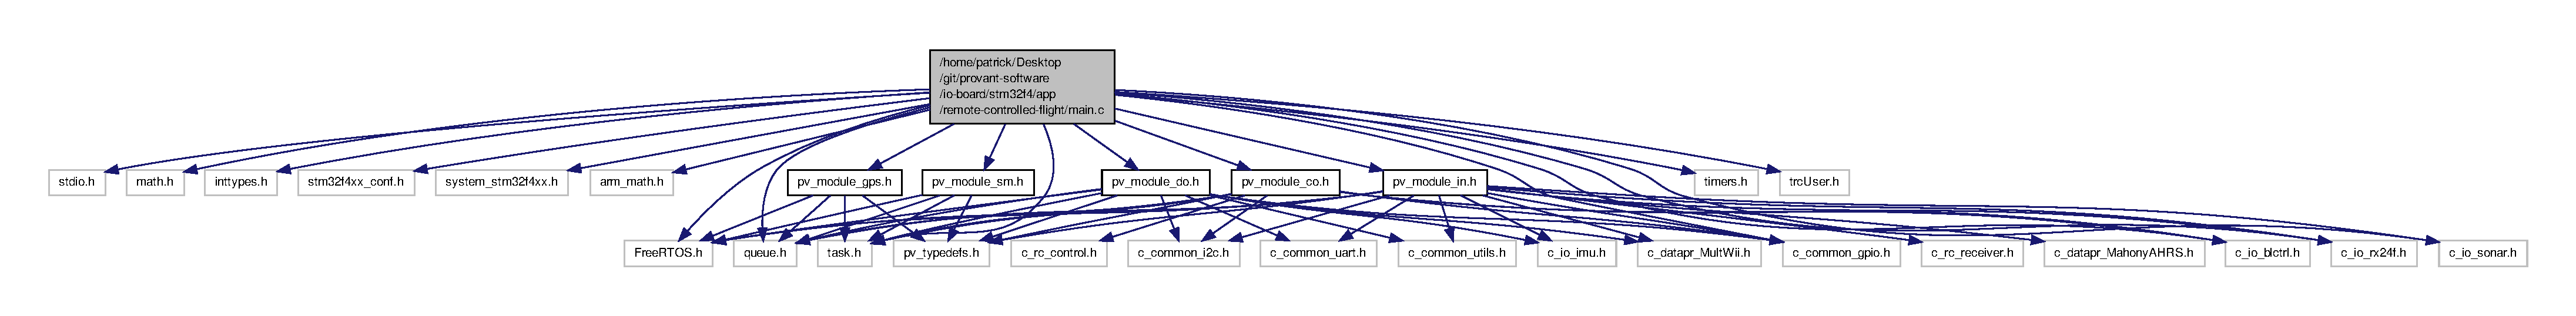
\includegraphics[width=350pt]{main_8c__incl}
\end{center}
\end{figure}
\subsection*{Macros}
\begin{DoxyCompactItemize}
\item 
\#define \hyperlink{main_8c_a42e162ee7b8b8c2663d1dbd31c7b590b}{A\-R\-M\-\_\-\-M\-A\-T\-H\-\_\-\-C\-M4}
\end{DoxyCompactItemize}
\subsection*{Funções}
\begin{DoxyCompactItemize}
\item 
void \hyperlink{group__ProVANT__Modules_ga2850b09d1bb227364b5ff6de6f85f740}{v\-Application\-Tick\-Hook} ()
\item 
void \hyperlink{group__ProVANT__Modules_ga11cbdd335da884dec1204e230554bfd9}{v\-Application\-Idle\-Hook} ()
\item 
void \hyperlink{group__ProVANT__Modules_ga8f5b98d87cfd1379b8d6573159bcbdd3}{v\-Application\-Stack\-Overflow\-Hook} ()
\item 
void \hyperlink{group__ProVANT__Modules_ga73f6aa45470ada02a5d6f3a522d8f13c}{v\-Application\-Malloc\-Failed\-Hook} ()
\item 
void \hyperlink{group__ProVANT__Modules_ga73e2a1fcfc7e7f2bb22937e543997019}{F\-P\-U\-\_\-init} ()
\item 
void \hyperlink{group__ProVANT__Modules_ga39e7a5088757fe328c0162fe25d907bf}{blink\-\_\-led\-\_\-task} (void $\ast$pv\-Parameters)
\item 
void \hyperlink{group__ProVANT__Modules_gab0c5d271dba436247302632e599731ba}{module\-\_\-co\-\_\-task} (void $\ast$pv\-Parameters)
\item 
void \hyperlink{group__ProVANT__Modules_ga7de15cbee9a0ca9eafb3eb25f5e3d691}{module\-\_\-in\-\_\-task} (void $\ast$pv\-Parameters)
\item 
void \hyperlink{group__ProVANT__Modules_ga466679da7a6953ce332271681ce397c7}{module\-\_\-do\-\_\-task} (void $\ast$pv\-Parameters)
\item 
void \hyperlink{group__ProVANT__Modules_gac55e5b60dffafe957dddc7aa452bfa9d}{module\-\_\-gps\-\_\-task} (void $\ast$pv\-Parameters)
\item 
void \hyperlink{group__ProVANT__Modules_gaad8bcaa035ca56eddd3ccbf522298711}{module\-\_\-sm\-\_\-task} (void $\ast$pv\-Parameters)
\item 
int \hyperlink{group__ProVANT__Modules_ga840291bc02cba5474a4cb46a9b9566fe}{main} (void)
\end{DoxyCompactItemize}


\subsection{Descrição detalhada}
Startup do projeto. \begin{DoxyAuthor}{Autor}
Martin Vincent Bloedorn \& Patrick José Pereira 
\end{DoxyAuthor}
\begin{DoxyVersion}{Versão}
V1.\-0.\-0 
\end{DoxyVersion}
\begin{DoxyDate}{Data}
27-\/\-August-\/2014 
\end{DoxyDate}
\begin{DoxyWarning}{Aviso}
Modificar os arquivos provant-\/software/io-\/board/stm32f4/common/modules/common/stm32f4xx\-\_\-conf.\-h provant-\/software/io-\/board/stm32f4/lib/cmsis/inc/stm32f4xx.\-h provant-\/software/io-\/board/stm32f4/lib/cmsis/inc/stm32f4xx\-\_\-conf.\-h dependendo da placa que esta trabalhando. Recompilando com\-: make allclean make T\-O\-D\-O 
\end{DoxyWarning}


Definido no ficheiro \hyperlink{main_8c_source}{main.\-c}.



\subsection{Documentação das macros}
\hypertarget{main_8c_a42e162ee7b8b8c2663d1dbd31c7b590b}{\index{main.\-c@{main.\-c}!A\-R\-M\-\_\-\-M\-A\-T\-H\-\_\-\-C\-M4@{A\-R\-M\-\_\-\-M\-A\-T\-H\-\_\-\-C\-M4}}
\index{A\-R\-M\-\_\-\-M\-A\-T\-H\-\_\-\-C\-M4@{A\-R\-M\-\_\-\-M\-A\-T\-H\-\_\-\-C\-M4}!main.c@{main.\-c}}
\subsubsection[{A\-R\-M\-\_\-\-M\-A\-T\-H\-\_\-\-C\-M4}]{\setlength{\rightskip}{0pt plus 5cm}\#define A\-R\-M\-\_\-\-M\-A\-T\-H\-\_\-\-C\-M4}}\label{main_8c_a42e162ee7b8b8c2663d1dbd31c7b590b}


Definido na linha 29 do ficheiro main.\-c.


\hypertarget{pv__module__co_8c}{\section{Referência ao ficheiro /home/iuro/git/provant-\/software/io-\/board/stm32f4/app/remote-\/controlled-\/flight/pv\-\_\-module\-\_\-co.c}
\label{pv__module__co_8c}\index{/home/iuro/git/provant-\/software/io-\/board/stm32f4/app/remote-\/controlled-\/flight/pv\-\_\-module\-\_\-co.\-c@{/home/iuro/git/provant-\/software/io-\/board/stm32f4/app/remote-\/controlled-\/flight/pv\-\_\-module\-\_\-co.\-c}}
}
{\ttfamily \#include \char`\"{}pv\-\_\-module\-\_\-co.\-h\char`\"{}}\\*
Diagrama de dependências de inclusão para pv\-\_\-module\-\_\-co.\-c\-:
\subsection*{Macros}
\begin{DoxyCompactItemize}
\item 
\#define \hyperlink{group__app__co_ga0ac6c9f2991b096e49c354e5cce6fae0}{M\-O\-D\-U\-L\-E\-\_\-\-P\-E\-R\-I\-O\-D}~10
\item 
\#define \hyperlink{group__app__co_gaec8246e954743c1eca3ed9d0b934bf8e}{E\-S\-C\-\_\-\-O\-N}~1
\item 
\#define \hyperlink{group__app__co_ga162e9e4abd94f1558733bbf17fca28e9}{S\-E\-R\-V\-O\-\_\-\-O\-N}~1
\end{DoxyCompactItemize}
\subsection*{Funções}
\begin{DoxyCompactItemize}
\item 
void \hyperlink{group__app__co_gabedb9a5c3739466a359c93b3585a3640}{module\-\_\-co\-\_\-init} ()
\begin{DoxyCompactList}\small\item\em Inicializacao do módulo de controle + output. \end{DoxyCompactList}\item 
void \hyperlink{group__app__co_gaab8216fc955d01b47e3431aae288d9d3}{module\-\_\-co\-\_\-run} ()
\begin{DoxyCompactList}\small\item\em Função principal do módulo de R\-C. \end{DoxyCompactList}\end{DoxyCompactItemize}
\subsection*{Variáveis}
\begin{DoxyCompactItemize}
\item 
port\-Tick\-Type \hyperlink{group__app__co_gaa8db3871cb5f64abbd94ddd5a1db73a6}{last\-Wake\-Time}
\item 
pv\-\_\-msg\-\_\-input \hyperlink{group__app__co_gac40b8cfe5fd2000670ad57fe3e75ec89}{i\-Input\-Data}
\item 
pv\-\_\-msg\-\_\-control\-Output \hyperlink{group__app__co_ga0a14ca4568444d2d76c256fa91585cdf}{o\-Control\-Output\-Data}
\end{DoxyCompactItemize}

\hypertarget{pv__module__co_8h}{\section{Referência ao ficheiro /home/patrick/\-Desktop/git/provant-\/software/io-\/board/stm32f4/app/remote-\/controlled-\/flight/pv\-\_\-module\-\_\-co.h}
\label{pv__module__co_8h}\index{/home/patrick/\-Desktop/git/provant-\/software/io-\/board/stm32f4/app/remote-\/controlled-\/flight/pv\-\_\-module\-\_\-co.\-h@{/home/patrick/\-Desktop/git/provant-\/software/io-\/board/stm32f4/app/remote-\/controlled-\/flight/pv\-\_\-module\-\_\-co.\-h}}
}
{\ttfamily \#include \char`\"{}Free\-R\-T\-O\-S.\-h\char`\"{}}\\*
{\ttfamily \#include \char`\"{}queue.\-h\char`\"{}}\\*
{\ttfamily \#include \char`\"{}task.\-h\char`\"{}}\\*
{\ttfamily \#include \char`\"{}c\-\_\-common\-\_\-gpio.\-h\char`\"{}}\\*
{\ttfamily \#include \char`\"{}c\-\_\-common\-\_\-i2c.\-h\char`\"{}}\\*
{\ttfamily \#include \char`\"{}c\-\_\-rc\-\_\-control.\-h\char`\"{}}\\*
{\ttfamily \#include \char`\"{}c\-\_\-io\-\_\-blctrl.\-h\char`\"{}}\\*
{\ttfamily \#include \char`\"{}c\-\_\-io\-\_\-rx24f.\-h\char`\"{}}\\*
{\ttfamily \#include \char`\"{}pv\-\_\-typedefs.\-h\char`\"{}}\\*
Diagrama de dependências de inclusão para pv\-\_\-module\-\_\-co.\-h\-:
\nopagebreak
\begin{figure}[H]
\begin{center}
\leavevmode
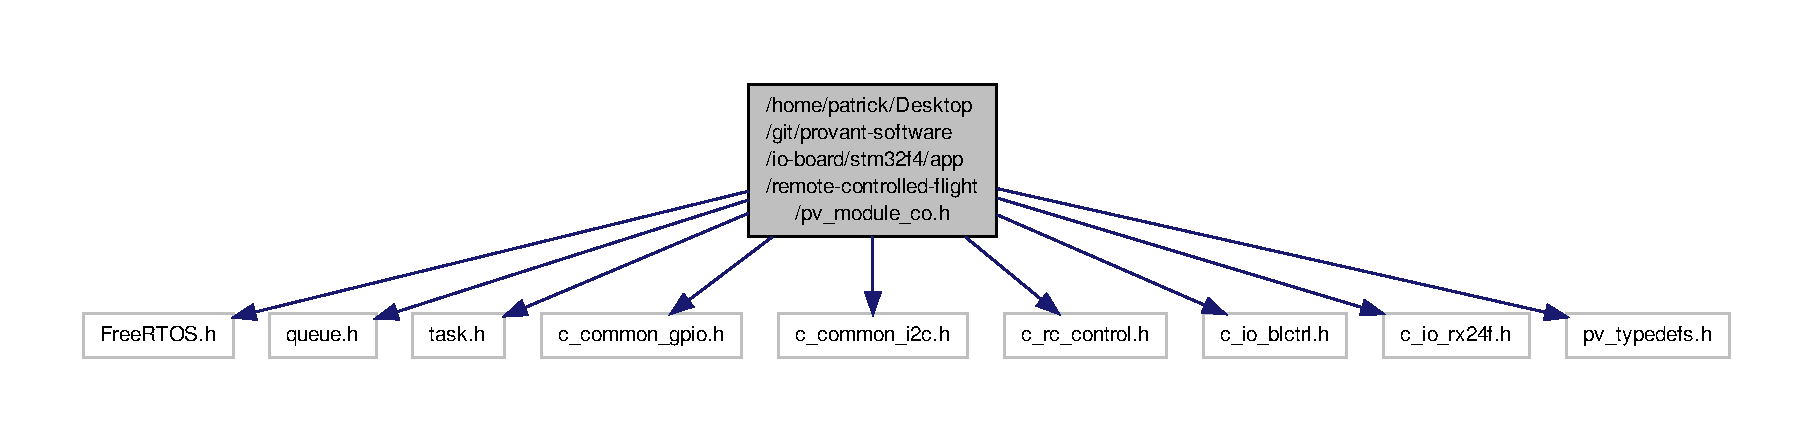
\includegraphics[width=350pt]{pv__module__co_8h__incl}
\end{center}
\end{figure}
Este grafo mostra quais são os ficheiros que incluem directamente ou indirectamente este ficheiro\-:
\nopagebreak
\begin{figure}[H]
\begin{center}
\leavevmode
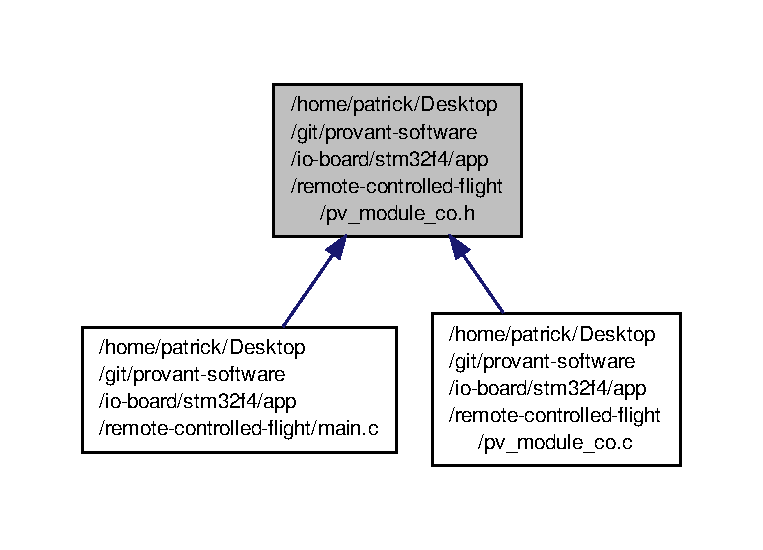
\includegraphics[width=350pt]{pv__module__co_8h__dep__incl}
\end{center}
\end{figure}
\subsection*{Estruturas de Dados}
\begin{DoxyCompactItemize}
\item 
struct \hyperlink{structpv__interface__co}{pv\-\_\-interface\-\_\-co}
\end{DoxyCompactItemize}
\subsection*{Funções}
\begin{DoxyCompactItemize}
\item 
void \hyperlink{group__Module__RC_gabedb9a5c3739466a359c93b3585a3640}{module\-\_\-co\-\_\-init} ()
\begin{DoxyCompactList}\small\item\em Inicializacao do módulo de R\-C. \end{DoxyCompactList}\item 
void \hyperlink{group__Module__RC_gaab8216fc955d01b47e3431aae288d9d3}{module\-\_\-co\-\_\-run} ()
\begin{DoxyCompactList}\small\item\em Função principal do módulo de R\-C. \end{DoxyCompactList}\end{DoxyCompactItemize}
\subsection*{Variáveis}
\begin{DoxyCompactItemize}
\item 
struct \hyperlink{structpv__interface__co}{pv\-\_\-interface\-\_\-co} \hyperlink{pv__module__co_8h_a452c8dc095e980ad1742c4c282fa4297}{pv\-\_\-interface\-\_\-co}
\end{DoxyCompactItemize}


\subsection{Documentação das variáveis}
\hypertarget{pv__module__co_8h_a452c8dc095e980ad1742c4c282fa4297}{\index{pv\-\_\-module\-\_\-co.\-h@{pv\-\_\-module\-\_\-co.\-h}!pv\-\_\-interface\-\_\-co@{pv\-\_\-interface\-\_\-co}}
\index{pv\-\_\-interface\-\_\-co@{pv\-\_\-interface\-\_\-co}!pv_module_co.h@{pv\-\_\-module\-\_\-co.\-h}}
\subsubsection[{pv\-\_\-interface\-\_\-co}]{\setlength{\rightskip}{0pt plus 5cm}struct {\bf pv\-\_\-interface\-\_\-co}  {\bf pv\-\_\-interface\-\_\-co}}}\label{pv__module__co_8h_a452c8dc095e980ad1742c4c282fa4297}

\hypertarget{pv__module__do_8c}{\section{Referência ao ficheiro /home/patrick/\-Desktop/git/provant-\/software/io-\/board/stm32f4/app/remote-\/controlled-\/flight/pv\-\_\-module\-\_\-do.c}
\label{pv__module__do_8c}\index{/home/patrick/\-Desktop/git/provant-\/software/io-\/board/stm32f4/app/remote-\/controlled-\/flight/pv\-\_\-module\-\_\-do.\-c@{/home/patrick/\-Desktop/git/provant-\/software/io-\/board/stm32f4/app/remote-\/controlled-\/flight/pv\-\_\-module\-\_\-do.\-c}}
}


Implementação do módulo de transmissao de dados para fora do A\-R\-M.  


{\ttfamily \#include \char`\"{}pv\-\_\-module\-\_\-do.\-h\char`\"{}}\\*
Diagrama de dependências de inclusão para pv\-\_\-module\-\_\-do.\-c\-:
\nopagebreak
\begin{figure}[H]
\begin{center}
\leavevmode
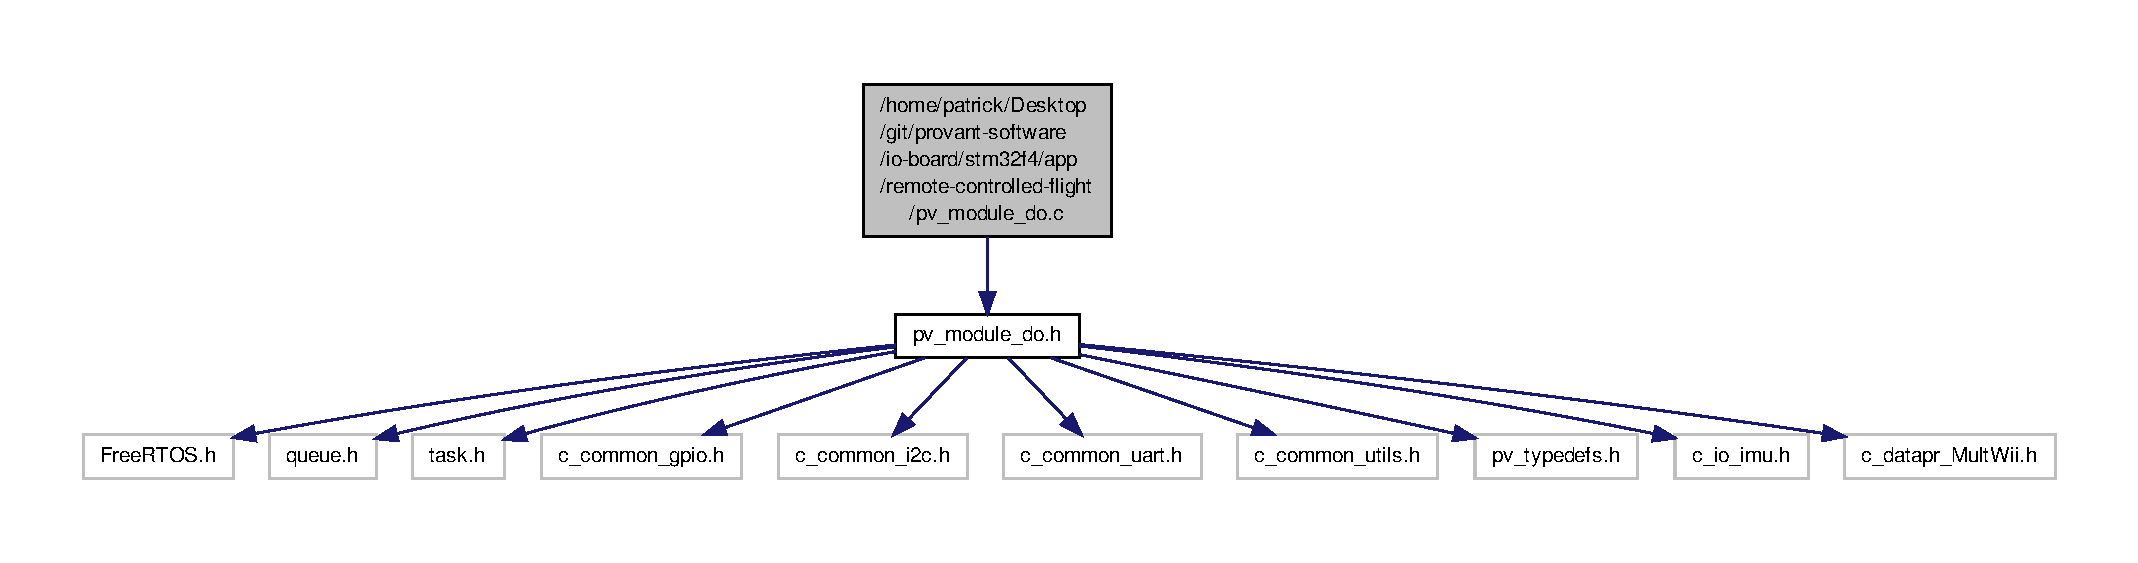
\includegraphics[width=350pt]{pv__module__do_8c__incl}
\end{center}
\end{figure}
\subsection*{Macros}
\begin{DoxyCompactItemize}
\item 
\#define \hyperlink{group__app__do_ga0ac6c9f2991b096e49c354e5cce6fae0}{M\-O\-D\-U\-L\-E\-\_\-\-P\-E\-R\-I\-O\-D}~100
\item 
\#define \hyperlink{group__app__do_ga6a53a6c94a70cc286e300a0ea8f46ba4}{U\-S\-A\-R\-T\-\_\-\-B\-A\-U\-D\-R\-A\-T\-E}~460800
\end{DoxyCompactItemize}
\subsection*{Funções}
\begin{DoxyCompactItemize}
\item 
void \hyperlink{group__app__do_ga901c023651503207f5cfd8cdb8c305b3}{module\-\_\-do\-\_\-init} ()
\begin{DoxyCompactList}\small\item\em Inicializacao do módulo de data out. \end{DoxyCompactList}\item 
void \hyperlink{group__app__do_ga1f08b4b431624465a47f47eca0520253}{module\-\_\-do\-\_\-run} ()
\begin{DoxyCompactList}\small\item\em Função principal do módulo de data out. \end{DoxyCompactList}\end{DoxyCompactItemize}
\subsection*{Variáveis}
\begin{DoxyCompactItemize}
\item 
port\-Tick\-Type \hyperlink{group__app__do_gaa8db3871cb5f64abbd94ddd5a1db73a6}{last\-Wake\-Time}
\item 
unsigned int \hyperlink{group__app__do_ga24475be702ffcc5a6f0a5557040368ef}{heart\-Beat} =0
\item 
pv\-\_\-msg\-\_\-input \hyperlink{group__app__do_gac40b8cfe5fd2000670ad57fe3e75ec89}{i\-Input\-Data}
\item 
pv\-\_\-msg\-\_\-control\-Output \hyperlink{group__app__do_gacabca53fbaffdbf13b8e5a1c29b73bc4}{i\-Control\-Output\-Data}
\end{DoxyCompactItemize}


\subsection{Descrição detalhada}
Implementação do módulo de transmissao de dados para fora do A\-R\-M. \begin{DoxyAuthor}{Autor}
Patrick Jose Pereira 
\end{DoxyAuthor}
\begin{DoxyVersion}{Versão}
V1.\-0.\-0 
\end{DoxyVersion}
\begin{DoxyDate}{Data}
27-\/\-August-\/2014 
\end{DoxyDate}


Definido no ficheiro \hyperlink{pv__module__do_8c_source}{pv\-\_\-module\-\_\-do.\-c}.


\hypertarget{pv__module__do_8h}{\section{Referência ao ficheiro /home/iuro/git/provant-\/software/io-\/board/stm32f4/app/remote-\/controlled-\/flight/pv\-\_\-module\-\_\-do.h}
\label{pv__module__do_8h}\index{/home/iuro/git/provant-\/software/io-\/board/stm32f4/app/remote-\/controlled-\/flight/pv\-\_\-module\-\_\-do.\-h@{/home/iuro/git/provant-\/software/io-\/board/stm32f4/app/remote-\/controlled-\/flight/pv\-\_\-module\-\_\-do.\-h}}
}


Implementação do módulo de transmissao de dados para fora do A\-R\-M.  


{\ttfamily \#include \char`\"{}Free\-R\-T\-O\-S.\-h\char`\"{}}\\*
{\ttfamily \#include \char`\"{}queue.\-h\char`\"{}}\\*
{\ttfamily \#include \char`\"{}task.\-h\char`\"{}}\\*
{\ttfamily \#include \char`\"{}c\-\_\-common\-\_\-gpio.\-h\char`\"{}}\\*
{\ttfamily \#include \char`\"{}c\-\_\-common\-\_\-i2c.\-h\char`\"{}}\\*
{\ttfamily \#include \char`\"{}c\-\_\-common\-\_\-uart.\-h\char`\"{}}\\*
{\ttfamily \#include \char`\"{}c\-\_\-common\-\_\-utils.\-h\char`\"{}}\\*
{\ttfamily \#include \char`\"{}pv\-\_\-typedefs.\-h\char`\"{}}\\*
{\ttfamily \#include \char`\"{}c\-\_\-io\-\_\-imu.\-h\char`\"{}}\\*
{\ttfamily \#include \char`\"{}c\-\_\-datapr\-\_\-\-Mult\-Wii.\-h\char`\"{}}\\*
Diagrama de dependências de inclusão para pv\-\_\-module\-\_\-do.\-h\-:
Este grafo mostra quais são os ficheiros que incluem directamente ou indirectamente este ficheiro\-:
\subsection*{Estruturas de Dados}
\begin{DoxyCompactItemize}
\item 
struct \hyperlink{structpv__interface__do}{pv\-\_\-interface\-\_\-do}
\end{DoxyCompactItemize}
\subsection*{Funções}
\begin{DoxyCompactItemize}
\item 
void \hyperlink{group__app__do_ga901c023651503207f5cfd8cdb8c305b3}{module\-\_\-do\-\_\-init} ()
\begin{DoxyCompactList}\small\item\em Inicializacao do módulo de data out. \end{DoxyCompactList}\item 
void \hyperlink{group__app__do_ga1f08b4b431624465a47f47eca0520253}{module\-\_\-do\-\_\-run} ()
\begin{DoxyCompactList}\small\item\em Função principal do módulo de data out. \end{DoxyCompactList}\end{DoxyCompactItemize}
\subsection*{Variáveis}
\begin{DoxyCompactItemize}
\item 
struct \hyperlink{structpv__interface__do}{pv\-\_\-interface\-\_\-do} \hyperlink{pv__module__do_8h_acdcb55c89a8823c672940a0901d30868}{pv\-\_\-interface\-\_\-do}
\end{DoxyCompactItemize}


\subsection{Descrição detalhada}
Implementação do módulo de transmissao de dados para fora do A\-R\-M. \begin{DoxyAuthor}{Autor}
Patrick Jose Pereira 
\end{DoxyAuthor}
\begin{DoxyVersion}{Versão}
V1.\-0.\-0 
\end{DoxyVersion}
\begin{DoxyDate}{Data}
27-\/\-August-\/2014 
\end{DoxyDate}


Definido no ficheiro \hyperlink{pv__module__do_8h_source}{pv\-\_\-module\-\_\-do.\-h}.



\subsection{Documentação das variáveis}
\hypertarget{pv__module__do_8h_acdcb55c89a8823c672940a0901d30868}{\index{pv\-\_\-module\-\_\-do.\-h@{pv\-\_\-module\-\_\-do.\-h}!pv\-\_\-interface\-\_\-do@{pv\-\_\-interface\-\_\-do}}
\index{pv\-\_\-interface\-\_\-do@{pv\-\_\-interface\-\_\-do}!pv_module_do.h@{pv\-\_\-module\-\_\-do.\-h}}
\subsubsection[{pv\-\_\-interface\-\_\-do}]{\setlength{\rightskip}{0pt plus 5cm}struct {\bf pv\-\_\-interface\-\_\-do}  {\bf pv\-\_\-interface\-\_\-do}}}\label{pv__module__do_8h_acdcb55c89a8823c672940a0901d30868}

\hypertarget{pv__module__gps_8c}{\section{Referência ao ficheiro /home/patrick/\-Desktop/git/provant-\/software/io-\/board/stm32f4/app/remote-\/controlled-\/flight/pv\-\_\-module\-\_\-gps.c}
\label{pv__module__gps_8c}\index{/home/patrick/\-Desktop/git/provant-\/software/io-\/board/stm32f4/app/remote-\/controlled-\/flight/pv\-\_\-module\-\_\-gps.\-c@{/home/patrick/\-Desktop/git/provant-\/software/io-\/board/stm32f4/app/remote-\/controlled-\/flight/pv\-\_\-module\-\_\-gps.\-c}}
}


Implementação do módulo de leitura de dados do G\-P\-S.  


{\ttfamily \#include \char`\"{}pv\-\_\-module\-\_\-gps.\-h\char`\"{}}\\*
Diagrama de dependências de inclusão para pv\-\_\-module\-\_\-gps.\-c\-:
\nopagebreak
\begin{figure}[H]
\begin{center}
\leavevmode
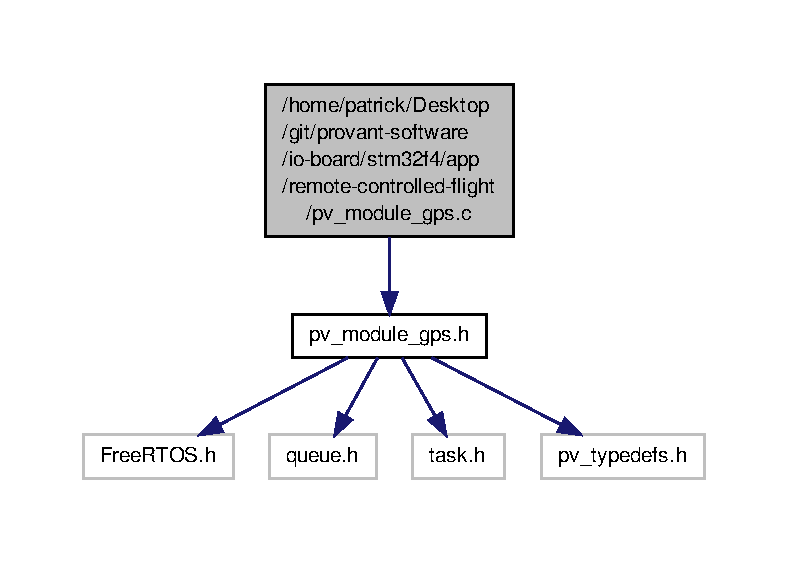
\includegraphics[width=350pt]{pv__module__gps_8c__incl}
\end{center}
\end{figure}
\subsection*{Macros}
\begin{DoxyCompactItemize}
\item 
\#define \hyperlink{group__app__gps_ga0ac6c9f2991b096e49c354e5cce6fae0}{M\-O\-D\-U\-L\-E\-\_\-\-P\-E\-R\-I\-O\-D}~100
\end{DoxyCompactItemize}
\subsection*{Funções}
\begin{DoxyCompactItemize}
\item 
void \hyperlink{group__app__gps_ga9ee93102a0a5aec6877376bbcaf1dcb0}{module\-\_\-gps\-\_\-init} ()
\begin{DoxyCompactList}\small\item\em Inicializacao do módulo de G\-P\-S. \end{DoxyCompactList}\item 
void \hyperlink{group__app__gps_gace423457cfae0d22bd57db9e2fb4c033}{module\-\_\-gps\-\_\-run} ()
\begin{DoxyCompactList}\small\item\em Função principal do módulo de G\-P\-S. \end{DoxyCompactList}\end{DoxyCompactItemize}
\subsection*{Variáveis}
\begin{DoxyCompactItemize}
\item 
port\-Tick\-Type \hyperlink{group__app__gps_gaa8db3871cb5f64abbd94ddd5a1db73a6}{last\-Wake\-Time}
\end{DoxyCompactItemize}


\subsection{Descrição detalhada}
Implementação do módulo de leitura de dados do G\-P\-S. \begin{DoxyAuthor}{Autor}
Patrick Jose Pereira 
\end{DoxyAuthor}
\begin{DoxyVersion}{Versão}
V1.\-0.\-0 
\end{DoxyVersion}
\begin{DoxyDate}{Data}
27-\/\-August-\/2014 
\end{DoxyDate}


Definido no ficheiro \hyperlink{pv__module__gps_8c_source}{pv\-\_\-module\-\_\-gps.\-c}.


\hypertarget{pv__module__gps_8h}{\section{Referência ao ficheiro /home/patrick/\-Desktop/git/provant-\/software/io-\/board/stm32f4/app/remote-\/controlled-\/flight/pv\-\_\-module\-\_\-gps.h}
\label{pv__module__gps_8h}\index{/home/patrick/\-Desktop/git/provant-\/software/io-\/board/stm32f4/app/remote-\/controlled-\/flight/pv\-\_\-module\-\_\-gps.\-h@{/home/patrick/\-Desktop/git/provant-\/software/io-\/board/stm32f4/app/remote-\/controlled-\/flight/pv\-\_\-module\-\_\-gps.\-h}}
}


Implementação do módulo de leitura de dados do G\-P\-S.  


{\ttfamily \#include \char`\"{}Free\-R\-T\-O\-S.\-h\char`\"{}}\\*
{\ttfamily \#include \char`\"{}queue.\-h\char`\"{}}\\*
{\ttfamily \#include \char`\"{}task.\-h\char`\"{}}\\*
{\ttfamily \#include \char`\"{}pv\-\_\-typedefs.\-h\char`\"{}}\\*
Diagrama de dependências de inclusão para pv\-\_\-module\-\_\-gps.\-h\-:
\nopagebreak
\begin{figure}[H]
\begin{center}
\leavevmode
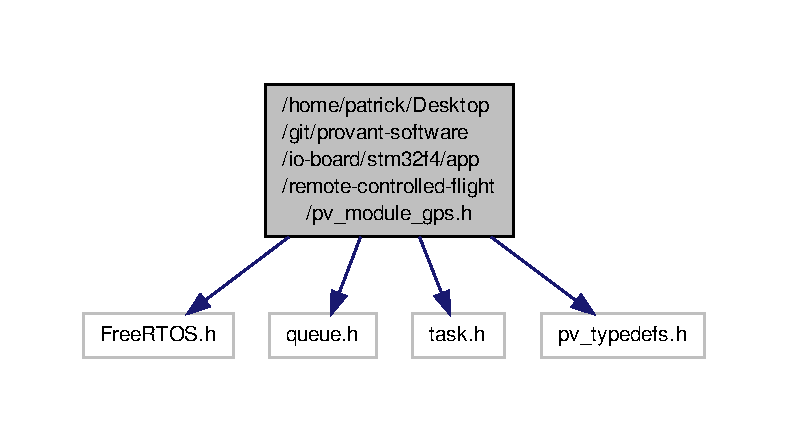
\includegraphics[width=350pt]{pv__module__gps_8h__incl}
\end{center}
\end{figure}
Este grafo mostra quais são os ficheiros que incluem directamente ou indirectamente este ficheiro\-:
\nopagebreak
\begin{figure}[H]
\begin{center}
\leavevmode
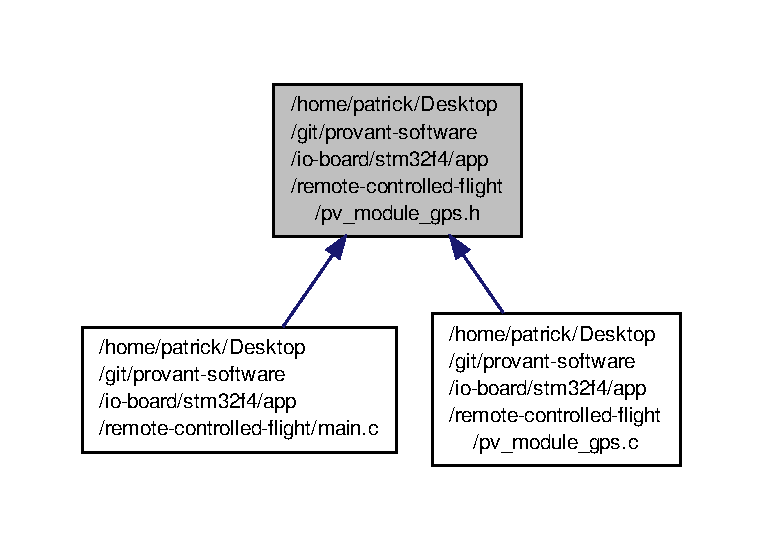
\includegraphics[width=350pt]{pv__module__gps_8h__dep__incl}
\end{center}
\end{figure}
\subsection*{Funções}
\begin{DoxyCompactItemize}
\item 
void \hyperlink{group__app__gps_ga9ee93102a0a5aec6877376bbcaf1dcb0}{module\-\_\-gps\-\_\-init} ()
\begin{DoxyCompactList}\small\item\em Inicializacao do módulo de G\-P\-S. \end{DoxyCompactList}\item 
void \hyperlink{group__app__gps_gace423457cfae0d22bd57db9e2fb4c033}{module\-\_\-gps\-\_\-run} ()
\begin{DoxyCompactList}\small\item\em Função principal do módulo de G\-P\-S. \end{DoxyCompactList}\end{DoxyCompactItemize}


\subsection{Descrição detalhada}
Implementação do módulo de leitura de dados do G\-P\-S. \begin{DoxyAuthor}{Autor}
Patrick Jose Pereira 
\end{DoxyAuthor}
\begin{DoxyVersion}{Versão}
V1.\-0.\-0 
\end{DoxyVersion}
\begin{DoxyDate}{Data}
27-\/\-August-\/2014 
\end{DoxyDate}


Definido no ficheiro \hyperlink{pv__module__gps_8h_source}{pv\-\_\-module\-\_\-gps.\-h}.


\hypertarget{pv__module__in_8c}{\section{Referência ao ficheiro /home/iuro/git/provant-\/software/io-\/board/stm32f4/app/remote-\/controlled-\/flight/pv\-\_\-module\-\_\-in.c}
\label{pv__module__in_8c}\index{/home/iuro/git/provant-\/software/io-\/board/stm32f4/app/remote-\/controlled-\/flight/pv\-\_\-module\-\_\-in.\-c@{/home/iuro/git/provant-\/software/io-\/board/stm32f4/app/remote-\/controlled-\/flight/pv\-\_\-module\-\_\-in.\-c}}
}
{\ttfamily \#include \char`\"{}pv\-\_\-module\-\_\-in.\-h\char`\"{}}\\*
Diagrama de dependências de inclusão para pv\-\_\-module\-\_\-in.\-c\-:
\subsection*{Macros}
\begin{DoxyCompactItemize}
\item 
\#define \hyperlink{group__app__in_ga0ac6c9f2991b096e49c354e5cce6fae0}{M\-O\-D\-U\-L\-E\-\_\-\-P\-E\-R\-I\-O\-D}~10
\end{DoxyCompactItemize}
\subsection*{Funções}
\begin{DoxyCompactItemize}
\item 
void \hyperlink{group__app__in_gaffe0980a750cbec13ebf241c933460dd}{module\-\_\-in\-\_\-init} ()
\begin{DoxyCompactList}\small\item\em Inicializacao componentes de I\-O. \end{DoxyCompactList}\item 
void \hyperlink{group__app__in_ga2b56089e4c5adb9ac8b7a41fc1a0b0b2}{module\-\_\-in\-\_\-run} ()
\begin{DoxyCompactList}\small\item\em Função principal do módulo de I\-O. \end{DoxyCompactList}\end{DoxyCompactItemize}
\subsection*{Variáveis}
\begin{DoxyCompactItemize}
\item 
port\-Tick\-Type \hyperlink{group__app__in_gaa8db3871cb5f64abbd94ddd5a1db73a6}{last\-Wake\-Time}
\item 
pv\-\_\-msg\-\_\-input \hyperlink{group__app__in_gaffc6f7805bab2d46af160c6f7715ba99}{o\-Input\-Data}
\end{DoxyCompactItemize}

\hypertarget{pv__module__in_8h}{\section{Referência ao ficheiro /home/iuro/git/provant-\/software/io-\/board/stm32f4/app/remote-\/controlled-\/flight/pv\-\_\-module\-\_\-in.h}
\label{pv__module__in_8h}\index{/home/iuro/git/provant-\/software/io-\/board/stm32f4/app/remote-\/controlled-\/flight/pv\-\_\-module\-\_\-in.\-h@{/home/iuro/git/provant-\/software/io-\/board/stm32f4/app/remote-\/controlled-\/flight/pv\-\_\-module\-\_\-in.\-h}}
}
{\ttfamily \#include \char`\"{}Free\-R\-T\-O\-S.\-h\char`\"{}}\\*
{\ttfamily \#include \char`\"{}queue.\-h\char`\"{}}\\*
{\ttfamily \#include \char`\"{}task.\-h\char`\"{}}\\*
{\ttfamily \#include \char`\"{}c\-\_\-common\-\_\-gpio.\-h\char`\"{}}\\*
{\ttfamily \#include \char`\"{}c\-\_\-common\-\_\-i2c.\-h\char`\"{}}\\*
{\ttfamily \#include \char`\"{}c\-\_\-common\-\_\-uart.\-h\char`\"{}}\\*
{\ttfamily \#include \char`\"{}c\-\_\-common\-\_\-utils.\-h\char`\"{}}\\*
{\ttfamily \#include \char`\"{}c\-\_\-io\-\_\-blctrl.\-h\char`\"{}}\\*
{\ttfamily \#include \char`\"{}c\-\_\-io\-\_\-rx24f.\-h\char`\"{}}\\*
{\ttfamily \#include \char`\"{}c\-\_\-io\-\_\-imu.\-h\char`\"{}}\\*
{\ttfamily \#include \char`\"{}c\-\_\-io\-\_\-sonar.\-h\char`\"{}}\\*
{\ttfamily \#include \char`\"{}c\-\_\-rc\-\_\-receiver.\-h\char`\"{}}\\*
{\ttfamily \#include \char`\"{}pv\-\_\-typedefs.\-h\char`\"{}}\\*
{\ttfamily \#include \char`\"{}c\-\_\-datapr\-\_\-\-Mult\-Wii.\-h\char`\"{}}\\*
{\ttfamily \#include \char`\"{}c\-\_\-datapr\-\_\-\-Mahony\-A\-H\-R\-S.\-h\char`\"{}}\\*
Diagrama de dependências de inclusão para pv\-\_\-module\-\_\-in.\-h\-:
Este grafo mostra quais são os ficheiros que incluem directamente ou indirectamente este ficheiro\-:
\subsection*{Estruturas de Dados}
\begin{DoxyCompactItemize}
\item 
struct \hyperlink{structpv__interface__in}{pv\-\_\-interface\-\_\-in}
\end{DoxyCompactItemize}
\subsection*{Macros}
\begin{DoxyCompactItemize}
\item 
\#define \hyperlink{pv__module__in_8h_a652f732918751d421cd00672fbcf34e6}{E\-N\-A\-B\-L\-E\-\_\-\-I\-M\-U}~1
\begin{DoxyCompactList}\small\item\em Define que modulos serao utilizados. \end{DoxyCompactList}\item 
\#define \hyperlink{pv__module__in_8h_ad825ce45a05b0e80e8d97f8cebd1ee76}{E\-N\-A\-B\-L\-E\-\_\-\-S\-E\-R\-V\-O}~0
\item 
\#define \hyperlink{pv__module__in_8h_a2cce57def91019d83715f42bb8927241}{E\-N\-A\-B\-L\-E\-\_\-\-E\-S\-C}~0
\item 
\#define \hyperlink{pv__module__in_8h_a18a3d20d2bd25a062405b951913ea276}{E\-N\-A\-B\-L\-E\-\_\-\-S\-O\-N\-A\-R}~0
\item 
\#define \hyperlink{pv__module__in_8h_acd356bc5fafb6cf72fd434275f0026a6}{E\-N\-A\-L\-B\-E\-\_\-\-D\-E\-B\-U\-G}~1
\end{DoxyCompactItemize}
\subsection*{Funções}
\begin{DoxyCompactItemize}
\item 
void \hyperlink{group__app__in_gaffe0980a750cbec13ebf241c933460dd}{module\-\_\-in\-\_\-init} ()
\begin{DoxyCompactList}\small\item\em Inicializacao componentes de I\-O. \end{DoxyCompactList}\item 
void \hyperlink{group__app__in_ga2b56089e4c5adb9ac8b7a41fc1a0b0b2}{module\-\_\-in\-\_\-run} ()
\begin{DoxyCompactList}\small\item\em Função principal do módulo de I\-O. \end{DoxyCompactList}\end{DoxyCompactItemize}
\subsection*{Variáveis}
\begin{DoxyCompactItemize}
\item 
struct \hyperlink{structpv__interface__in}{pv\-\_\-interface\-\_\-in} \hyperlink{pv__module__in_8h_adb91b9002b5ee35e4d9c1b0a1eb2b6e3}{pv\-\_\-interface\-\_\-in}
\end{DoxyCompactItemize}


\subsection{Documentação das macros}
\hypertarget{pv__module__in_8h_a2cce57def91019d83715f42bb8927241}{\index{pv\-\_\-module\-\_\-in.\-h@{pv\-\_\-module\-\_\-in.\-h}!E\-N\-A\-B\-L\-E\-\_\-\-E\-S\-C@{E\-N\-A\-B\-L\-E\-\_\-\-E\-S\-C}}
\index{E\-N\-A\-B\-L\-E\-\_\-\-E\-S\-C@{E\-N\-A\-B\-L\-E\-\_\-\-E\-S\-C}!pv_module_in.h@{pv\-\_\-module\-\_\-in.\-h}}
\subsubsection[{E\-N\-A\-B\-L\-E\-\_\-\-E\-S\-C}]{\setlength{\rightskip}{0pt plus 5cm}\#define E\-N\-A\-B\-L\-E\-\_\-\-E\-S\-C~0}}\label{pv__module__in_8h_a2cce57def91019d83715f42bb8927241}


Definido na linha 28 do ficheiro pv\-\_\-module\-\_\-in.\-h.

\hypertarget{pv__module__in_8h_a652f732918751d421cd00672fbcf34e6}{\index{pv\-\_\-module\-\_\-in.\-h@{pv\-\_\-module\-\_\-in.\-h}!E\-N\-A\-B\-L\-E\-\_\-\-I\-M\-U@{E\-N\-A\-B\-L\-E\-\_\-\-I\-M\-U}}
\index{E\-N\-A\-B\-L\-E\-\_\-\-I\-M\-U@{E\-N\-A\-B\-L\-E\-\_\-\-I\-M\-U}!pv_module_in.h@{pv\-\_\-module\-\_\-in.\-h}}
\subsubsection[{E\-N\-A\-B\-L\-E\-\_\-\-I\-M\-U}]{\setlength{\rightskip}{0pt plus 5cm}\#define E\-N\-A\-B\-L\-E\-\_\-\-I\-M\-U~1}}\label{pv__module__in_8h_a652f732918751d421cd00672fbcf34e6}


Define que modulos serao utilizados. 

Se E\-N\-A\-B\-L\-E\-\_\-$\ast$ 1 então tal modulo será utilizado 

Definido na linha 26 do ficheiro pv\-\_\-module\-\_\-in.\-h.

\hypertarget{pv__module__in_8h_ad825ce45a05b0e80e8d97f8cebd1ee76}{\index{pv\-\_\-module\-\_\-in.\-h@{pv\-\_\-module\-\_\-in.\-h}!E\-N\-A\-B\-L\-E\-\_\-\-S\-E\-R\-V\-O@{E\-N\-A\-B\-L\-E\-\_\-\-S\-E\-R\-V\-O}}
\index{E\-N\-A\-B\-L\-E\-\_\-\-S\-E\-R\-V\-O@{E\-N\-A\-B\-L\-E\-\_\-\-S\-E\-R\-V\-O}!pv_module_in.h@{pv\-\_\-module\-\_\-in.\-h}}
\subsubsection[{E\-N\-A\-B\-L\-E\-\_\-\-S\-E\-R\-V\-O}]{\setlength{\rightskip}{0pt plus 5cm}\#define E\-N\-A\-B\-L\-E\-\_\-\-S\-E\-R\-V\-O~0}}\label{pv__module__in_8h_ad825ce45a05b0e80e8d97f8cebd1ee76}


Definido na linha 27 do ficheiro pv\-\_\-module\-\_\-in.\-h.

\hypertarget{pv__module__in_8h_a18a3d20d2bd25a062405b951913ea276}{\index{pv\-\_\-module\-\_\-in.\-h@{pv\-\_\-module\-\_\-in.\-h}!E\-N\-A\-B\-L\-E\-\_\-\-S\-O\-N\-A\-R@{E\-N\-A\-B\-L\-E\-\_\-\-S\-O\-N\-A\-R}}
\index{E\-N\-A\-B\-L\-E\-\_\-\-S\-O\-N\-A\-R@{E\-N\-A\-B\-L\-E\-\_\-\-S\-O\-N\-A\-R}!pv_module_in.h@{pv\-\_\-module\-\_\-in.\-h}}
\subsubsection[{E\-N\-A\-B\-L\-E\-\_\-\-S\-O\-N\-A\-R}]{\setlength{\rightskip}{0pt plus 5cm}\#define E\-N\-A\-B\-L\-E\-\_\-\-S\-O\-N\-A\-R~0}}\label{pv__module__in_8h_a18a3d20d2bd25a062405b951913ea276}


Definido na linha 29 do ficheiro pv\-\_\-module\-\_\-in.\-h.

\hypertarget{pv__module__in_8h_acd356bc5fafb6cf72fd434275f0026a6}{\index{pv\-\_\-module\-\_\-in.\-h@{pv\-\_\-module\-\_\-in.\-h}!E\-N\-A\-L\-B\-E\-\_\-\-D\-E\-B\-U\-G@{E\-N\-A\-L\-B\-E\-\_\-\-D\-E\-B\-U\-G}}
\index{E\-N\-A\-L\-B\-E\-\_\-\-D\-E\-B\-U\-G@{E\-N\-A\-L\-B\-E\-\_\-\-D\-E\-B\-U\-G}!pv_module_in.h@{pv\-\_\-module\-\_\-in.\-h}}
\subsubsection[{E\-N\-A\-L\-B\-E\-\_\-\-D\-E\-B\-U\-G}]{\setlength{\rightskip}{0pt plus 5cm}\#define E\-N\-A\-L\-B\-E\-\_\-\-D\-E\-B\-U\-G~1}}\label{pv__module__in_8h_acd356bc5fafb6cf72fd434275f0026a6}


Definido na linha 30 do ficheiro pv\-\_\-module\-\_\-in.\-h.



\subsection{Documentação das variáveis}
\hypertarget{pv__module__in_8h_adb91b9002b5ee35e4d9c1b0a1eb2b6e3}{\index{pv\-\_\-module\-\_\-in.\-h@{pv\-\_\-module\-\_\-in.\-h}!pv\-\_\-interface\-\_\-in@{pv\-\_\-interface\-\_\-in}}
\index{pv\-\_\-interface\-\_\-in@{pv\-\_\-interface\-\_\-in}!pv_module_in.h@{pv\-\_\-module\-\_\-in.\-h}}
\subsubsection[{pv\-\_\-interface\-\_\-in}]{\setlength{\rightskip}{0pt plus 5cm}struct {\bf pv\-\_\-interface\-\_\-in}  {\bf pv\-\_\-interface\-\_\-in}}}\label{pv__module__in_8h_adb91b9002b5ee35e4d9c1b0a1eb2b6e3}

\hypertarget{pv__module__sm_8c}{\section{Referência ao ficheiro /home/iuro/git/provant-\/software/io-\/board/stm32f4/app/remote-\/controlled-\/flight/pv\-\_\-module\-\_\-sm.c}
\label{pv__module__sm_8c}\index{/home/iuro/git/provant-\/software/io-\/board/stm32f4/app/remote-\/controlled-\/flight/pv\-\_\-module\-\_\-sm.\-c@{/home/iuro/git/provant-\/software/io-\/board/stm32f4/app/remote-\/controlled-\/flight/pv\-\_\-module\-\_\-sm.\-c}}
}


Implementação do módulo da maquinas de estados do V\-A\-N\-T.  


{\ttfamily \#include \char`\"{}pv\-\_\-module\-\_\-sm.\-h\char`\"{}}\\*
Diagrama de dependências de inclusão para pv\-\_\-module\-\_\-sm.\-c\-:
\subsection*{Macros}
\begin{DoxyCompactItemize}
\item 
\#define \hyperlink{group__app__sm_ga0ac6c9f2991b096e49c354e5cce6fae0}{M\-O\-D\-U\-L\-E\-\_\-\-P\-E\-R\-I\-O\-D}~20
\end{DoxyCompactItemize}
\subsection*{Funções}
\begin{DoxyCompactItemize}
\item 
void \hyperlink{group__app__sm_gaf1b95b5ff451c9c5d9a4cdd34531201b}{module\-\_\-sm\-\_\-init} ()
\begin{DoxyCompactList}\small\item\em Inicializacao do módulo de sm. \end{DoxyCompactList}\item 
void \hyperlink{group__app__sm_ga81e54a060d460608697719ba6afab1e4}{module\-\_\-sm\-\_\-run} ()
\begin{DoxyCompactList}\small\item\em Função principal do módulo da sm. \end{DoxyCompactList}\end{DoxyCompactItemize}
\subsection*{Variáveis}
\begin{DoxyCompactItemize}
\item 
port\-Tick\-Type \hyperlink{group__app__sm_gaa8db3871cb5f64abbd94ddd5a1db73a6}{last\-Wake\-Time}
\end{DoxyCompactItemize}


\subsection{Descrição detalhada}
Implementação do módulo da maquinas de estados do V\-A\-N\-T. \begin{DoxyAuthor}{Autor}
Patrick Jose Pereira 
\end{DoxyAuthor}
\begin{DoxyVersion}{Versão}
V1.\-0.\-0 
\end{DoxyVersion}
\begin{DoxyDate}{Data}
27-\/\-August-\/2014 
\end{DoxyDate}


Definido no ficheiro \hyperlink{pv__module__sm_8c_source}{pv\-\_\-module\-\_\-sm.\-c}.


\hypertarget{pv__module__sm_8h}{\section{Referência ao ficheiro /home/patrick/\-Desktop/git/provant-\/software/io-\/board/stm32f4/app/remote-\/controlled-\/flight/pv\-\_\-module\-\_\-sm.h}
\label{pv__module__sm_8h}\index{/home/patrick/\-Desktop/git/provant-\/software/io-\/board/stm32f4/app/remote-\/controlled-\/flight/pv\-\_\-module\-\_\-sm.\-h@{/home/patrick/\-Desktop/git/provant-\/software/io-\/board/stm32f4/app/remote-\/controlled-\/flight/pv\-\_\-module\-\_\-sm.\-h}}
}


Implementação do módulo da maquinas de estados do V\-A\-N\-T.  


{\ttfamily \#include \char`\"{}Free\-R\-T\-O\-S.\-h\char`\"{}}\\*
{\ttfamily \#include \char`\"{}queue.\-h\char`\"{}}\\*
{\ttfamily \#include \char`\"{}task.\-h\char`\"{}}\\*
{\ttfamily \#include \char`\"{}pv\-\_\-typedefs.\-h\char`\"{}}\\*
Diagrama de dependências de inclusão para pv\-\_\-module\-\_\-sm.\-h\-:
\nopagebreak
\begin{figure}[H]
\begin{center}
\leavevmode
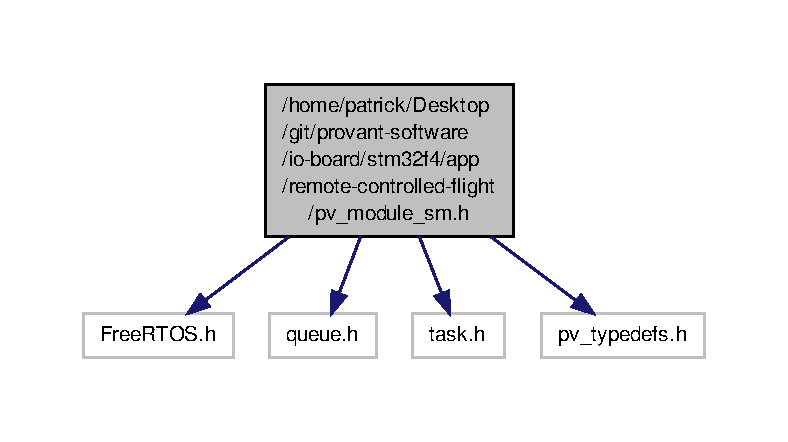
\includegraphics[width=350pt]{pv__module__sm_8h__incl}
\end{center}
\end{figure}
Este grafo mostra quais são os ficheiros que incluem directamente ou indirectamente este ficheiro\-:
\nopagebreak
\begin{figure}[H]
\begin{center}
\leavevmode
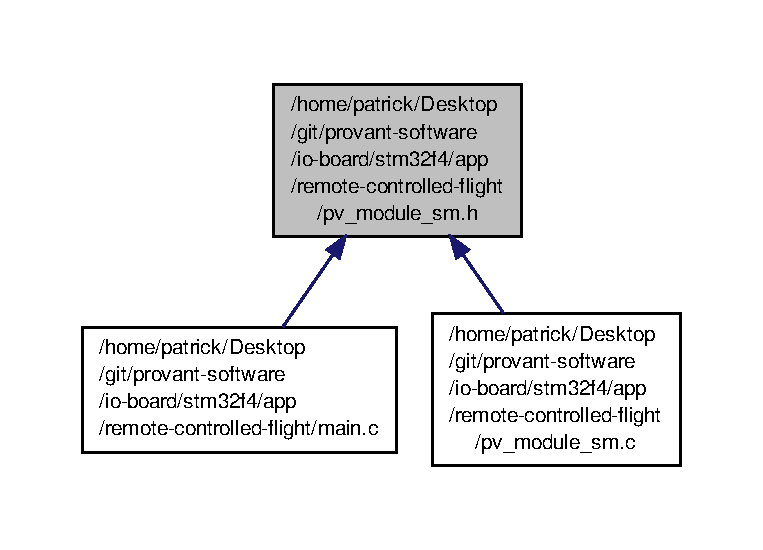
\includegraphics[width=350pt]{pv__module__sm_8h__dep__incl}
\end{center}
\end{figure}
\subsection*{Funções}
\begin{DoxyCompactItemize}
\item 
void \hyperlink{group__app__sm_gaf1b95b5ff451c9c5d9a4cdd34531201b}{module\-\_\-sm\-\_\-init} ()
\begin{DoxyCompactList}\small\item\em Inicializacao do módulo de sm. \end{DoxyCompactList}\item 
void \hyperlink{group__app__sm_ga81e54a060d460608697719ba6afab1e4}{module\-\_\-sm\-\_\-run} ()
\begin{DoxyCompactList}\small\item\em Função principal do módulo da sm. \end{DoxyCompactList}\end{DoxyCompactItemize}


\subsection{Descrição detalhada}
Implementação do módulo da maquinas de estados do V\-A\-N\-T. \begin{DoxyAuthor}{Autor}
Patrick Jose Pereira 
\end{DoxyAuthor}
\begin{DoxyVersion}{Versão}
V1.\-0.\-0 
\end{DoxyVersion}
\begin{DoxyDate}{Data}
27-\/\-August-\/2014 
\end{DoxyDate}


Definido no ficheiro \hyperlink{pv__module__sm_8h_source}{pv\-\_\-module\-\_\-sm.\-h}.


%--- End generated contents ---

% Index
\newpage
\phantomsection
\addcontentsline{toc}{part}{Índice}
\printindex

\end{document}
